% TODO Change language to en_GB (recommended) or en_US for English documents
\documentclass[11pt,a4paper,oneside]{report}
\usepackage{mathtools}             % Single-side
%\documentclass[11pt,a4paper,twoside,openright]{report}  % Duplex

% thanks to http://tex.stackexchange.com/a/47579/71109
\usepackage{ifxetex}
\usepackage{ifluatex}
\newif\ifxetexorluatex % a new conditional starts as false
\ifnum 0\ifxetex 1\fi\ifluatex 1\fi>0
   \xetexorluatextrue
\fi

\ifxetexorluatex
  \usepackage{fontspec}
\else
  \usepackage[T1]{fontenc}
  \usepackage[utf8]{inputenc}
  \usepackage[lighttt]{lmodern}
  \ttfamily\DeclareFontShape{T1}{lmtt}{m}{it}{<->sub*lmtt/m/sl}{}
\fi

\usepackage[english,magyar]{babel} % Alapértelmezés szerint utoljára definiált nyelv lesz aktív, de később külön beállítjuk az aktív nyelvet.

\usepackage{emptypage} % omit page number on empty pages

%\usepackage{cmap}
\usepackage{amsfonts,amsmath,amssymb} % Mathematical symbols.
%\usepackage[ruled,boxed,resetcount,linesnumbered]{algorithm2e} % For pseudocodes. % beware: this is not compatible with LuaLaTeX, see http://tex.stackexchange.com/questions/34814/lualatex-and-algorithm2e
\usepackage{booktabs} % For publication quality tables for LaTeX
\usepackage{graphicx}

%\usepackage{fancyhdr}
%\usepackage{lastpage}

\usepackage{geometry}
%\usepackage{sectsty}
\usepackage{setspace} % For setting line spacing

\usepackage[unicode]{hyperref} % For hyperlinks in the generated document.
\usepackage{xcolor}
\usepackage{listings} % For source code snippets.

\usepackage[amsmath,thmmarks]{ntheorem} % Theorem-like environments.

\usepackage[hang]{caption}

\singlespacing

\newcommand{\selecthungarian}{
	\selectlanguage{magyar}
	\setlength{\parindent}{2em}
	\setlength{\parskip}{0em}
	\frenchspacing
}

\newcommand{\selectenglish}{
	\selectlanguage{english}
	\setlength{\parindent}{0em}
	\setlength{\parskip}{0.5em}
	\nonfrenchspacing
	\renewcommand{\figureautorefname}{Figure}
	\renewcommand{\tableautorefname}{Table}
	\renewcommand{\partautorefname}{Part}
	\renewcommand{\chapterautorefname}{Chapter}
	\renewcommand{\sectionautorefname}{Section}
	\renewcommand{\subsectionautorefname}{Section}
	\renewcommand{\subsubsectionautorefname}{Section}
}

\usepackage[numbers]{natbib}
\usepackage{xspace}

\newcommand{\vikszerzoVezeteknev}{Józsa}
\newcommand{\vikszerzoKeresztnev}{György Bence}

\newcommand{\vikkonzulensAMegszolitas}{}
\newcommand{\vikkonzulensAVezeteknev}{Sárközy}
\newcommand{\vikkonzulensAKeresztnev}{Péter}

\newcommand{\vikkonzulensBMegszolitas}{}
\newcommand{\vikkonzulensBVezeteknev}{}
\newcommand{\vikkonzulensBKeresztnev}{}

\newcommand{\vikkonzulensCMegszolitas}{}
\newcommand{\vikkonzulensCVezeteknev}{}
\newcommand{\vikkonzulensCKeresztnev}{}

\newcommand{\vikcim}{Using unsupervised clustering methods on the latent space of drug-like molecules} % Cím
\newcommand{\viktanszek}{\bmemit} % Tanszék
\newcommand{\vikdoktipus}{\bsc} % Dokumentum típusa (\bsc vagy \msc)
\newcommand{\vikmunkatipusat}{szakdolgozatot} % a "hallgató nyilatkozat" részhez: szakdolgozatot vagy diplomatervet

\input{include/tdk-variables}
\newcommand{\szerzoMeta}{\vikszerzoVezeteknev{} \vikszerzoKeresztnev} % egy szerző esetén
%\newcommand{\szerzoMeta}{\vikszerzoVezeteknev{} \vikszerzoKeresztnev, \tdkszerzoB} % két szerző esetén

% Settings for English documents
\input{include/thesis-en}

\input{include/preamble}

%--------------------------------------------------------------------------------------
% Table of contents and the main text
%--------------------------------------------------------------------------------------
\begin{document}

\pagenumbering{gobble}

\selectthesislanguage

%~~~~~~~~~~~~~~~~~~~~~~~~~~~~~~~~~~~~~~~~~~~~~~~~~~~~~~~~~~~~~~~~~~~~~~~~~~~~~~~~~~~~~~
\include{include/titlepage}		   % Szakdolgozat/Diplomaterv címlap


% Table of Contents
%~~~~~~~~~~~~~~~~~~~~~~~~~~~~~~~~~~~~~~~~~~~~~~~~~~~~~~~~~~~~~~~~~~~~~~~~~~~~~~~~~~~~~~
\tableofcontents\cleardoublepage


% Declaration and Abstract
%~~~~~~~~~~~~~~~~~~~~~~~~~~~~~~~~~~~~~~~~~~~~~~~~~~~~~~~~~~~~~~~~~~~~~~~~~~~~~~~~~~~~~~
\pagenumbering{roman}
\setcounter{page}{1}

\selecthungarian

%----------------------------------------------------------------------------
% Abstract in Hungarian
%----------------------------------------------------------------------------
\chapter*{Kivonat}\addcontentsline{toc}{chapter}{Kivonat}

A modern gyógyszerkutatás egyik legfőbb motivációja az gyógyszerként viselkedő vegyületek előállítása. Az új gyógyszermolekulák felfedezése lehetővé teszi az eddig gyógyíthatatlannak vélt betegségek kezelését. A \textit{de novo} molekulagenerálás egy olyan folyamat, mely során egy adott, molekulákat tartalmazó adathalmaz alapján generálunk molekulákat, amelyek az adatbázisban lévőekhez hasonlóak, de azoktól eltérőek. Ez a módszer az utóbbi évtizedekben egyre népszerűbbé vált.

Az új gyógyszerszerű molekulák előállítása nagyon költséges és időigényes. A folyamat felgyorsítására az elmúlt három évtizedben a gépi tanulást és a mély neurális hálózatokat alkalmazták. Különösen népszerű módszer a variációs autoenkóder használata a célzott keresésre alkalmas gyógyszerszerű molekulák látens terének létrehozására.

Egy ilyen látens tér azonban csak akkor használható, ha az a molekulák kémiai szerkezetére nézve sima. Ennek eldöntése azonban nem triviális, mivel a molekulák kémiai szerkezete nem könnyen számszerűsíthető, és az ilyen látens tereknek általában magas a dimenzionalitása, ami miatt szükséges dimenzió redukciós és vizualizáló algorithmusok használata.

Az elmúlt évtizedekben számos dimenzió redukciós és vizualizációs algoritmust fejlesztettek ki. A dolgozatomban öt gyakran használt algoritmust - PCA, t-SNE, UMAP, TriMAP és PaCMAP - vizsgálok meg, hogy mennyire használható eredményt adnak egy adott adathalmazra.

Mindegyik algoritmust abból a szempontból vizsgálom, hogy képesek-e egy 64 dimenziós látens teret úgy átalakítani, hogy az így kapott kétdimenziós tér a molekulák kémiai szerkezetére nézve sima legyen. Optimalizálom az egyes algoritmusok hiperparamétereit, ezzel vizsgálva, hogy hogyan alakítják át a kapott beágyazást, és elvégzek egy LERP-tesztet a teljes tér leképzésének vizsgálatára.



\vfill
\selectenglish


%----------------------------------------------------------------------------
% Abstract in English
%----------------------------------------------------------------------------
\chapter*{Abstract}\addcontentsline{toc}{chapter}{Abstract}

In modern drug research, one of the most important tasks is finding novel drug-like molecules. The discovery of new drug molecules makes it possible to treat diseases previously thought incurable. \textit{De novo} molecule design is the process of generating novel chemicals based on a dataset of drug-like molecules. This method has gained popularity in recent decades.

The cost of generating novel drug-like molecules is very costly and time-consuming. To speed the process up, machine learning and deep neural networks have been used in the last three decades. A particularly popular method is using a variational autoencoder to generate a latent space of drug-like molecules suitable for targeted searching.

Quantifying the quality of such a latent space is vital for effective usage. This task is not trivial however, as the chemical structure of molecules cannot be easily quantized and such latent spaces tend to be high-dimensional, leading to the need for dimension reducing visualization algorithms to be applied.

Many dimension reduction and visualization algorithms have been developed in recent decades. In this paper, I evaluate five commonly used algorithms -- PCA, t-SNE, UMAP, TriMAP and PaCMAP -- to see how well they perform on a given dataset.

I examine each algorithm on their ability to transform a 64-dimensional latent space such that the resulting two-dimensional space is smooth over chemical structure. I optimize  the hyperparameters of each algorithm to see how they transform the resulting embedding, and perform a LERP test to see how they map the entire space into two dimensions.


\vfill
\cleardoublepage

\selectthesislanguage

\newcounter{romanPage}
\setcounter{romanPage}{\value{page}}
\stepcounter{romanPage}    %TODO Összefoglaló -- TDK és OTDK esetén nem kötelező


% The main part of the thesis
%~~~~~~~~~~~~~~~~~~~~~~~~~~~~~~~~~~~~~~~~~~~~~~~~~~~~~~~~~~~~~~~~~~~~~~~~~~~~~~~~~~~~~~
\pagenumbering{arabic}

%TODO import your own content
%----------------------------------------------------------------------------
\chapter{\bevezetes}\label{ch:introduction}
%----------------------------------------------------------------------------

\section{Motivation}\label{sec:motivation}

Computational bio- and chemoinformatics often requires the usage and processing of high-dimensional data. Working with such data poses certain challenges however. While some datasets are constructed with meaningful and easily interpretable feature sets, often times the dimensions carry no direct interpretation, forming a \textit{latent space} of data points.

High dimensionality introduces redundancy in the representation of data points. It is also undesirable as the time of operations scale with the number of dimensions in the dataset.

Latent representation of data is advantageous for eliminating redundancy in the dataset. This is because features taken from real descriptors (such as number of carbon atoms in a molecule and molar mass) are often not independent of each other. These correlations of dimensions lead to spaces of lower dimension with near equivalent descriptive power to the original space.

High dimensionality also poses challenges in interpreting data. Correlations between features, or sets of features become difficult to discover as the number of potential pairings increase. Datasets with more than three dimensions pose additional challenges as visualizing such datasets is difficult and often impractical, rendering visual interpretation methods unusable.

\section{Exploring the chemical space}\label{sec:exploring-the-chemical-space}

One of the more important goals of modern pharmaceutical research is the discovery of novel drug-like molecules. This development however is a long and costly process. The entire procedure can in some cases take 20 years~\cite{bib:rndprod}, and may cost as much as 2.6 billion dollars~\cite{bib:2.6billion}. During the development, thousands of potential compounds are being tested, of which only half a dozen candidates will reach clinical trials, where their effects are tested in humans. In most cases, only one drug is approved so that it can reach doctors and patients.

In order to reduce the time cost of the procedure, as well as the financial cost, targeted search of the chemical space is necessary. This conclusion is also supported by the fact that while scientists have successfully synthesised millions of molecules with molar weight less than 500, the number of potential such molecules may be $10^{24}$, or according to some estimates, even $10^{60}$~\cite{bib:1060}, making random searches of the chemical space effectively impossible.

Using targeted searching on the space of drug-like molecules is a heavily researched topic. Algorithms exist, however, finding efficient searching algorithms without enumerating every element of the subspace is difficult. Deep neural networks have been used for \textit{de novo} molecule generation with promising results~\cite{bib:molsearch}. One particularly promising method is the use of VAE's \textit{variational autoencoders}~\cite{bib:vae} to transform the chemical space into a latent space that is smooth over chemical structure.

The number of dimensions of an autoencoder's latent space is usually between 32 and 128, which is rather large, and carries the challenges in the understanding of the underlying structure presented in section~\ref{sec:motivation}. The analysis of such latent spaces is important for finding novel molecules with desirable drug-like properties.

\section{Unsupervised clustering}\label{sec:unsupervised-clustering}

In data science, a very common task is discovering similarities and dissimilarities between data points. Categorizing points of data is perhaps the most obvious example of this, however, more general tasks exist in datasets where no such clean categories exist. These problems require a more general solution for representing similarities of points.

Cluster analysis is the grouping of objects such that objects in the same cluster are more similar to each other than they are to objects in another cluster. The classification into clusters is done using criteria such as smallest distances, density of data points, graphs, or various statistical distributions. Cluster analysis has  wide applicability, including in unsupervised machine learning, data mining, statistics, graph analytics,  image processing, and numerous physical and social science applications.

Clustering is used to identify groups of similar objects in datasets with two or more variable quantities. In practice, this data may be collected from marketing, biomedical, or geospatial databases, among datasets that come from preprocessing such databases.

Clustering is often used to discover underlying structure in data through \textit{unsupervised learning}. No labels are given to the learning algorithm, leaving it on its own to find structure in its input. Unsupervised learning can be a goal in itself (discovering hidden patterns in data) or a means towards an end (feature learning).

\section{Outline of work}


In my thesis, I examine five dimension reduction algorithms, namely PCA, t-SNE, UMAP, TriMAP and PaCMAP. In chapter (\ref{ch:dimension-reduction-algorithms}), I introduce each algorithm, and provide simple description of how they work. I will also present a basic comparison of based on these descriptions. 

In chapter (\ref{ch:resources}), I talk about the resources that I had during my work. This includes the hardware on which I ran the algorithms and the software packages that I used, including the implementations of all algorithms presented. I also describe the dataset that I used in my investigation.

Following that in chapter (\ref{ch:own-work}), I compare the algorithms in detail, running them with different parametrization on the latent dataset of drug-like molecules. With optimizing parameters and running tests, I examine which unsupervised clustering algorithm works best on the given dataset.

Finally, in chapter (\ref{ch:conclusion}), I summarize my findings and talk about future plans.
%----------------------------------------------------------------------------
\chapter{Dimension reduction algorithms}\label{ch:dimension-reduction-algorithms}
%----------------------------------------------------------------------------

For completeness, this chapter contains the theoretical background of PCA, t-SNE, UMAP, TriMAP and PaCMAP in common notation. After introducing every algorithm, their advantages and disadvantages are listed. At the end of the chapter, I compare these algorithms on a theoretical basis without my results working on the dataset detailed in~\ref{sec:used-data}.

$\mathbf{X} \in \mathbb{R}^{N\times M}$ is used to denote the original dataset, for which an embedding $\mathbf{Y} \in \mathbb{R}^{N\times K}$ is constructed. For each observation $i \in [N]$, $\mathbf{x}_i$ and $\mathbf{y}_i$ is used to denote its corresponding representation in $\mathbf{X}$ and $\mathbf{Y}$ respectively. $\mathbf{x}_i$ is a given value and $\mathbf{y}_i$ is a $K$-dimensional decision variable. The distance between $\mathbf{x}_i$ and $\mathbf{x}_j$, which is used as a measure of similarity between the points is denoted by $d(\mathbf{x}_i, \mathbf{x}_j)$. This distance metric may be defined differently between methods, but it is always a metric in $\mathbb{R}^{K}$.

\section{PCA}\label{sec:pca}

\textit{Principal Component Analysis}\cite{bib:pca}, or PCA for short is the most widespread dimension reduction algorithm. It works by finding \textit{principal components}. These are a series of $p$ unit vectors, where the $i$-th vector minimizes the average squared distance from the points to the line, while also being orthogonal to the first $i - 1$ vectors.

PCA is the process of computing the principal components of the data and performing a change of basis, usually using only the first few principal components and ignoring the rest. This leads to a lower dimensional representation of the data, where only the components that preserve as much of the data's variation as possible.

\subsection{Mathematical details}\label{subsec:mathematical-details}

The goal of the PCA algorithm is to find unit basis vectors $\mathbf{w}_{(i)}$, such that the projected data inherits the maximum possible variance of the original data matrix $\mathbf{X}$.

The first vector $\mathbf{w}_{(1)}$ has to satisfy

\begin{equation}
	\mathbf{w}_{(1)} = \arg\max_{\lVert \mathbf{w} \rVert = 1}{ \Bigg\{ \sum_i{ \big(\mathbf{x}_{(i)} \cdot \mathbf{w} \big)^2 } \Bigg\} }
	\label{eq:pca:w1}
\end{equation}

The $k$-th component can be found by subtracting the first $k - 1$ components from $\mathbf{X}$

\begin{equation}
	\mathbf{\hat{X}}_{k}=\mathbf{X}-\sum_{s=1}^{k-1}\mathbf{X}\mathbf{w}_{(s)}\mathbf{w}_{(s)}^{\mathsf{T}}
	\label{eq:pca_xhat}
\end{equation}

and then computing the first principal component of the new matrix:

\begin{equation}
	\mathbf{w}_{(k)}=\arg\max_{\lVert \mathbf{w} \rVert = 1}{\Bigg\{ \lVert \mathbf{\hat {X}}_{k}\mathbf{w} \rVert ^2 \Bigg\} }
	\label{eq:pca:wk}
\end{equation}

The projected dataset is given by the following linear transformation:

\begin{equation}
	\mathbf{T} = \mathbf{XW}
	\label{eq:pca:t}
\end{equation}

\subsection{Benefits of PCA}\label{subsec:benefits-of-pca}

The popularity of PCA lies in its ease of use. It is easily accessible for data science use-cases, with a variety of implementations in a number of environments.

The application of PCA on a given dataset is trivial. The only parameter of the algorithm is the output dimension, and the result is a deterministic function of the dataset.\footnote{In practice this is not entirely true, since the search for $\mathbf{w}_{(i)}$ given by equation~\eqref{eq:pca:w1} cannot be implemented without some error.} This means that using PCA does not involve fine-tuning hyper-parameters, which can take a long time and takes away the focus from understanding the underlying data.

Furthermore, the PCA algorithm is simple, without any computationally expensive steps. This results in an algorithm that uses minimal hardware resources. Even working with large datasets, no supercomputer is needed for the application of principal component analysis.

\subsection{Limitations of PCA}\label{subsec:limitations-of-pca}


PCA has a number of limitations that make it unfavourable to us in certain use-cases. These limitations arise from certain assumptions made in its derivation.

One such assumption is the standardization of the used dataset. This means that the scaling of variables affect the result of PCA. Differently scaled features not only change the outcome of the transformation, but there is also a high likelihood of information loss. This can be counteracted by scaling the features of the dataset by its standard deviation, however, this is not always desirable.

Another assumption made is that the dataset contains only linear dependencies. PCA can capture linear correlations between the features but cannot capture nonlinear dependencies between them. In some cases, a transformation of the coordinates, such that the resulting representation only contains linear correlations between features, may enable PCA to successfully capture such dependencies. This is the basis for a generalization of the technique called \textit{nonlinear PCA}\cite{bib:nonlinpca}. This however requires a function that transforms the initial dataset to an entirely linearly dependent representation, which can be difficult to find, and in some cases is impossible.

\section{t-SNE}\label{sec:t-sne}

\textit{t-distributed stochastic neighbour embedding}\cite{bib:tsne}, abbreviated to t-SNE is one of the more widely methods for visualizing high dimensional data in usually two or three dimensions. The technique is based on stochastic neighbour embedding\cite{bib:sne} but utilising Student's t-distribution.

\subsection{Algorithm}

t-SNE consists of two main stages. The first one is constructing a probability distribution over pairs of high dimensional objects such that similar points are assigned higher probabilities while dissimilar objects are assigned lower probability. In the second stage, t-SNE constructs a similar probability distribution over the points in the low-dimensional map, then minimises the  Kullback–Leibler divergence\cite{bib:kldiv} between the two distributions with respect to the positions of points in the map. The original version of t-SNE uses Euclidean distance as a metric for similarity, however, this can be changed in popular implementations where a different metric is more appropriate.

In the first step of the algorithm, a probability distribution is constructed over the pairs of high dimensional objects. The exact formula for the probability assigned to the pair $\mathbf{x}_i$ and $\mathbf{x}_j$ is given by

\begin{equation}
	\label{eq:tsne:pi|j}
	p_{i|j} =
	\begin{cases}
		{\frac {\exp(-\lVert \mathbf {x} _{i}-\mathbf {x} _{j}\rVert ^{2}/2\sigma _{i}^{2})}{\sum _{k\neq i}\exp(-\lVert \mathbf {x} _{i}-\mathbf {x} _{k}\rVert ^{2}/2\sigma _{i}^{2})}} & \textrm{if } i \neq j \\
		\hfil 0 & \textrm{if } i = j
	\end{cases}
\end{equation}

Van der Maaten and Hilton in their paper\cite{bib:tsne} give a very good explanation for this probability. ``The similarity of data point $\mathbf{x}_j$ to data point $\mathbf{x}_i$ is the conditional probability, $p_{j|i}$, that $\mathbf{x}_i$ would pick $\mathbf{x}_j$ as its neighbour if neighbours were picked in proportion to their probability density under a Gaussian centred at $\mathbf{x}_i$.''

Since this formula depends on the order of points ($p_{i|j} \neq p_{j|i}$), we define

\begin{equation}
	\label{eq:tsne:pij}
	p_{ij}={\frac {p_{j\mid i}+p_{i\mid j}}{2N}}
\end{equation}

where $N$ is the number of data points. Note that $p_{ij} = p_{ji}$, $p_{ii} = 0$ and $\displaystyle\sum_{i, j}p_{ij} = 1$.

The value of $\sigma_{i}$ is set in such a way that the \textit{perplexity} of the conditional distribution equals the predefined perplexity value given to t-SNE as a hyperparameter. Specifically, SNE performs a binary search for the value of $\sigma_{i}$ that produces probability distribution with a fixed perplexity that is specified by the user. This perplexity is calculated by the following formula:

\begin{equation}
	\label{eq:tsne:perlexity}
	Perplexity = 2^{-\sum_{p_{j|i}} \log_2 p_{j|i}}
\end{equation}

For the lower dimensional map, a similar probability distribution is constructed over pairs of low dimensional point pairs.

\begin{equation}
	\label{eq:tsne:qij}
	q_{ij} =
	\begin{cases}
		{\frac{(1+\lVert \mathbf{y}_{i} - \mathbf{y}_{j}\rVert^{2})^{-1}}{\sum_{k}\sum_{l \neq k}(1+\lVert \mathbf{y}_{k} - \mathbf{y}_{l}\rVert ^{2})^{-1}}} & \textrm{if } i \neq j \\
		\hfil 0 & \textrm{if } i = j
	\end{cases}
\end{equation}

Herein a heavy-tailed \textit{Student's t-distribution} is used to measure the similarity between low-dimensional points in order to allow dissimilar objects to be modelled far apart in the map.

The \textit{Kullback-Leibler divergence} (KL-divergence)\cite{bib:kldiv} of the probability distributions $P$ and $Q$ is then calculated as an error function:

\begin{equation}
	\label{eq:KLdiv}
 	\mathrm{KL} \left(P \parallel Q \right) = \sum_{i\neq j} p_{ij} \log{\frac{p_{ij}}{q_{ij}}}
\end{equation}

According to the original paper~\cite{bib:tsne}, the output matrix $Y$ is initialized using the multivariate Normal distribution  $\mathcal{N}(0,10^{-4}I)$, where $I$ denotes the $K$-dimensional identity matrix, and $K$ is the dimension of the output of t-SNE. In practice however, different initializations are utilised. One popular initialization is PCA, as it efficiently explores linear correlations between features of data.

The final locations of the points $\mathrm{y}_i$ in the map are determined by minimising the Kullback-Leibler divergence of the probability distributions with respect to the points $\mathrm{y}_i$. This minimization is performed by gradient descent~\cite{bib:gd}. The result of this optimization is a map that reflects the similarities between the high-dimensional inputs.

\subsection{Advantages over PCA}

t-SNE is a nonlinear dimensionality reduction algorithm, and as such can be used on datasets with nonlinear dependencies -- relationships in the data that PCA cannot capture. This property is essential in applications in computational chemistry, \textit{de novo} molecule generation and bioinformatics, where gathered data is rarely linear in nature.

Using t-SNE does not require standardization of data, as the used metric is the distance of data points. This however is not an advantage in cases where the data used is already standardized.

The algorithm has many hyperparameters, such as perplexity, and all parameters of gradient descent, such as learning rate, early exaggeration and number of iterations. This means that data scientists can ``tinker'' with t-SNE to find an embedding suitable for their use-case.

\subsection{Disadvantages}

The greatest drawback of using t-SNE lies in its extensive time and computation requirement. This is due in part to gradient descent, but the main reason for it is the use of computationally intensive operations, which will be detailed in section~\ref{sec:umap}. t-SNE does not scale well for larger datasets for this reason. Attempts to speed it up with \textit{FItSNE}\cite{bib:tsne:FItSNE} lead to large memory consumption, making it impossible to do analysis outside of computer clusters. On large datasets, using t-SNE requires powerful computers with large amounts of RAM and strong processors, or even GPU resources to be able to embed data points to a lower dimensional representation in sensible time.

Another disadvantage of using t-SNE -- which is not uniquely a property of t-SNE -- is the time investment of finding optimal hyperparameters. Particularly unfit parameters result in an embedding where clusters do not even form, and points of data translate to be randomly placed in the output space.\cite{bib:distill}

The t-SNE algorithm produces maps that do not preserve global structure of data. This means that while distances within clusters are a meaningful indicator for similarity, distances between clusters carry little to no meaning. This also means that t-SNE can translate similar points into two or more clusters.

t-SNE can practically only embed into two or three dimensions, which means it is only useful for visualization purposes, not general dimension reduction. This is still a problem for the more modern FItSNE algorithm.

\section{UMAP}\label{sec:umap}

\textit{Uniform Manifold Approximation and Projection}\cite{bib:umap}, or UMAP for short is a dimension reduction algorithm developed by Leland McInnes, John Healy and James Melville in 2018. It is constructed from a theoretical framework based in Riemannian geometry and algebraic topology. This technique was developed to overcome the shortcomings of t-SNE. The result is an algorithm that is competitive with t-SNE for visualization quality, arguably preserves more global structure and has superior run time performance. UMAP also has no restrictions on embedding dimension, making it suitable for general dimension reduction use cases.

The theoretical description of UMAP works in terms of \textit{fuzzy simplicial sets}, which are higher-dimensional generalizations of directed graphs, partially ordered sets and categories. Indeed, from a practical computational perspective, UMAP can ultimately be described in terms of, construction of, and operations on, weighted graphs. This puts UMAP in the class of k-neighbour based graph learning algorithms such as Laplacian Eigenmaps~\cite{bib:laplacian_eigenmaps}, Isomap~\cite{bib:isomap}, or t-SNE.

The theoretical description of the algorithm uses a few basic assumptions. For completeness, these are:

\begin{itemize}
	\item There exists a manifold on which the data would be uniformly distributed.
	\item The underlying manifold of interest is locally connected.
	\item Preserving the topological structure of this manifold is the primary goal.
\end{itemize}

\subsection{Algorithm}

There are many similarities between the t-SNE and UMAP algorithm. Both techniques consist of two distinct phases, which are similar in many ways and as such the most effective way to understand UMAP is to highlight the differences between the two.

The first phase of UMAP is constructing a high dimensional graph over the point of data using k-neighbour search, in order to approximate the topology of the dataset.

The first step in constructing the higher dimensional weighted graph is finding the $k$ nearest neighbours for every observation for a given distance metric $d(\mathbf{x}_i, \mathbf{x}_j)$. This metric is \textit{typically} Euclidean, however, most implementations offer other metrics. For every data point, the minimum positive distance from observation $i$ to a neighbour is calculated as $\rho_i$. In mathematical terms:

\begin{equation}
	\rho_i = \min \left\lbrace  d(\mathbf{x}_i, \mathbf{x}_{i_j}) \vert 1 \leq j \leq k, d(\mathbf{x}_i, \mathbf{x}_{i_j}) > 0 \right\rbrace
\end{equation}

After this, $\sigma_{i}$ is computed for every data point, by solving the equation:

\begin{equation}
	\log_2(k)=\sum_{j=1}^{k}\exp\left({\frac{-\max\{0,d(\mathbf{x}_i, \mathbf{x}_j)-\rho_i\}}{\sigma_i}}\right),
\end{equation}

or in a slightly different form:

\begin{equation}
	k=2^{\sum_{j=1}^{k}\exp\left({\frac{-\max\{0,d(\mathbf{x}_i, \mathbf{x}_j)-\rho_i\}}{\sigma_i}}\right)}.
\end{equation}

This computation is the counterpart of equation~\eqref{eq:tsne:perlexity} of t-SNE. Note that this equation does not contain a $\log_2$ component, which is computationally expensive, resulting in the computation of $\sigma_i$ being faster in the UMAP algorithm.

The weight function is defined between $\mathbf{x}_i$ and $\mathbf{x}_j$:

\begin{equation}
	w(\mathbf{x}_i, \mathbf{x}_j) = \exp\left({\frac{-\max\{0,d(\mathbf{x}_i, \mathbf{x}_j) - \rho_i\}} {\sigma_i}} \right).
\end{equation}

Note that this is weight function serves the same purpose as $p_{i|j}$ in t-SNE. A seemingly small but important difference between  the two formulas is the omission of normalization. This has dramatic effect on performance, since summation and integration are computationally expensive operations.

The weighted graph $G$ is defined whose vertices are individual observations from $\mathbf{X}$ and where for each edge $(i, j)$ it holds that $\mathbf{x}_i$ is a nearest neighbour of $\mathbf{x}_j$, or vice versa. The weight of an edge $(i, j)$ is the symmetrization of $w(\mathbf{x}_i, \mathbf{x}_j)$ and $w(\mathbf{x}_j, \mathbf{x}_i)$. This symmetric weight is defined as:

\begin{equation}
	\bar{w}_{i,j} = w(\mathbf{x}_i,\mathbf{x}_j)+w(\mathbf{x}_j,\mathbf{x}_i)-w(\mathbf{x}_i,\mathbf{x}_j)\cdot w(\mathbf{x}_j,\mathbf{x}_i).
\end{equation}

Note that this $G$ graph is analogous to t-SNE's $P$ probability distribution matrix.

The second phase of UMAP is the construction and optimization of output matrix (graph) $Y$. The initialization is performed canonically by using spectral embedding. As with t-SNE, implementations of UMAP usually offer different initialization options.

UMAP uses a force directed graph layout algorithm to optimise $Y$. This algorithm applies attractive forces along edges in $G$ and repulsive forces along $\bar{G}$, the complement of $G$. For every edge $(i, j)$ in $G$, the attractive force is defined as:

\begin{equation}
	\alpha\cdot
	\frac{-2ab\|\mathbf{y}_i-\mathbf{y}_j\|_2^{2(b-1)}}{1+a\left(\|\mathbf{y}_i-\mathbf{y}_j\|_2^{2}\right)^b}
	\bar{w}_{i,j}(\mathbf{y}_i-\mathbf{y}_j),
\end{equation}

while for every edge $(i, k)$  that is not in $G$, the following repulsive force is calculated:

\begin{equation}
	\alpha\cdot
	\frac{b}{\left(\epsilon+\|\mathbf{y}_i-\mathbf{y}_k\|_2^2\right)\left(1+a\left(\|\mathbf{y}_i-\mathbf{y}_k\|_2^{2}\right)^b\right)}
	\left(1- \bar{w}_{i,k}\right)(\mathbf{y}_i-\mathbf{y}_k),
\end{equation}

where $\epsilon$ is a small positive constant, to prevent division by zero.

The hyperparameters $a$ and $b$ are tuned using the data by fitting the function $\left(1+a\left(\|\mathbf{y}_i-\mathbf{y}_j\|_2^{2}\right)^b\right)^{-1}$ to the non-normalized weight function $\exp\left({-\max\{0,d(\mathbf{x}_i, \mathbf{x}_j)-\rho_i\}}\right)$ with the goal of creating a smooth approximation. The hyperparameter $\alpha$ indicates the learning rate. This family of curves is similar to Student's t-distribution used by t-SNE~\eqref{eq:tsne:qij}, but without integration in the denominator. This speeds up the calculation.

The last major difference between the t-SNE algorithm and UMAP is that while the former uses regular gradient descent~\cite{bib:gd}, UMAP uses stochastic gradient descent~\cite{bib:sgd}. This both speeds up the computations and consumes less memory.

\subsection{Advantages}

UMAP has quite a few advantages over PCA and t-SNE. As a nonlinear dimension reduction algorithm, UMAP is able to discover nonlinear correlations in the dataset, just like t-SNE. However, while practical application of t-SNE is only feasible in two or three dimensions due to tree-based algorithms for nearest neighbour search such as Barnes-Hut simulation~\cite{bib:barnes-hut}, UMAP has no such limitations, making it useful for general dimension reduction use-cases.

While UMAP also has many hyperparameters, these are more intuitive than that of t-SNE. Specifically, the perplexity parameter of t-SNE is only indirectly affecting $\sigma_i$, while UMAP's \texttt{n\_neighbour} parameter has a direct effect on $\sigma_i$. This means that users can more intuitively tune the algorithm for their use-cases.

In terms of performance, UMAP has been designed to run faster that t-SNE by omitting computationally expensive calculations and replacing them with similar but more easily executable formulas. This approach does not sacrifice quality of embedding while simultaneously speeding up calculations.

UMAP also consumes less memory overall, since instead of gradient descent, it uses stochastic gradient descent, therefore it needs to keep the gradients for only a subset of the observations.

The last and often overlooked advantage of UMAP lies in its derivation. UMAP is rigorously built from mathematical foundations, proving every step of the algorithm. As opposed to all other algorithms from this paper (with the exception of PCA), UMAP's steps are mathematically proven to work, and do not rely on a heuristic approach.

\subsection{Shortcomings}

As do all dimension reduction algorithms, UMAP has certain disadvantages when used on some datasets. Similarly to t-SNE, UMAP is a \textit{near-sighted} algorithm, meaning while it is very capable of preserving local structure of the input space, it struggles to preserve global structure. This however is not as severe in  UMAP as in t-SNE, since the hyperparameter \texttt{n\_neighbour}, which determines the number of nearest neighbours in the initial phase of the algorithm when set to large values, results in an embedding with more global structure preserved. This however can increase memory usage of the algorithm.

The computational representation of $k$-nearest neighbour search builds a matrix with $N \times N \times k$ values. With large datasets, increasing $k$ leads to large memory requirements, especially since with large values of $N$, preserving global structure requires an even larger $k$ value than for a smaller $N$. In practice, this leads to projection of large datasets resulting in less global structure preservation.

\section{TriMAP}\label{sec:trimap}

Both t-SNE and UMAP are considered near-sighted algorithms, meaning they preserve only local structure as opposed to global structure. While PCA is designed to preserve global structure, it suffers from limitations of nonlinear correlations. TriMAP~\cite{bib:trimap} is a graph-based nonlinear dimension reduction algorithm that aims to improve global structure preservation by using triplets of data points instead of pairs.



\subsection{Algorithm}

The algorithm defines triplets $(i, j, k)$ such that $d(\mathbf{x}_i, \mathbf{x}_j) < d(\mathbf{x}_i, \mathbf{x}_k)$. A subset of all triplets $\mathcal{T} \coloneqq \left\lbrace (i,j,k) \right\rbrace$ is used to approximate the structure of the dataset.

$\mathcal{T}$ is constructed in the following way:

\begin{itemize}
	\item For each observation $i$, \texttt{n\_inliers} nearest neighbour is found according to the distance metric used.
	\item For every sample $i$ and one of its neighbour $j$, \texttt{n\_outliers} points $k$ are sampled that are not neighbours of $i$.
	\item For each point $i$, two points are randomly sampled to make a triplet. This is repeated \texttt{n\_random} times.
	\item This results in set $\mathcal{T}$ that contains $\vert \mathcal{T} \vert = (\texttt{n\_inliers} \cdot \texttt{n\_outliers} + \texttt{n\_random}) \cdot N$ triplets.
\end{itemize}

The loss function is defined in multiple steps. The first one is the definition of $s(\mathbf{y}_i, \mathbf{y}_j)$ the following way:

\begin{equation}
	s(\mathbf{y}_i,\mathbf{y}_j)=\left(1+\|\mathbf{y}_i-\mathbf{y}_j\|^2\right)^{-1}
\end{equation}

This is very similar to UMAP's formula for finding its hyperparameters $a$ and $b$, and to t-SNE's Student's t-distribution.

A weight $w_{i,j,k}$ is defined for every triplet.

\begin{equation}
	\omega_{i,j,k} = \log\left(1+500\left(\frac{e^{d^2_{i,k}-d^2_{i,j}}}{\max_{(i',j',k')\in\mathcal{T}} e^{d^2_{i',k'}-d^2_{i',j'}}}+10^{-4}\right)\right),
\end{equation}

where $d^2_{i,j}$ is defined as

\begin{equation}
	\label{eq:trimap:d2}
	d^2_{i,j} = \frac{d^2(\mathbf{x}_i, \mathbf{x}_j)}{\sigma_i\sigma_j},
\end{equation}

and $\sigma_i$ is the average distance between $\mathbf{x}_i$ and the set of its 4--6 nearest neighbours.

Intuitively, $\omega_{i,j,k}$ is larger when the distances in the tuple are more significant, suggesting that it is more important to preserve this relation in the low-dimensional space.

For every triplet, a certain loss value can be calculated:

\begin{equation}
	l_{i,j,k}=\omega_{i,j,k}\frac{s(\mathbf{y}_i,\mathbf{y}_k)}{s(\mathbf{y}_i,\mathbf{y}_j)+s(\mathbf{y}_i,\mathbf{y}_k)}
\end{equation}

Note that $\omega_{i,j,k}$ is a static value which is only needed to calculate once based on the higher dimensional input triplets. $s(\mathbf{y}_i, \mathbf{y}_j)$ approaches 1 then $\mathbf{y}_i$ and $\mathbf{y}_j$ are closer and approaches 0 if the points are very distant.  This implies that the fraction in the triplet loss function would approach the maximal value of 1 when $i$ is placed close to $k$ and far away from $j$ (which contradicts the definition of a triplet $(i,j,k)$ where $i$ should be closer to $j$ than to $k$). Otherwise, as $k$ moves further away, the loss approaches 0.

For the total loss of the embedding the individual triplet loss values are summed.

\begin{equation}
	l_{\text{\tiny TriMAP}} = \sum_{(i,j,k)\in\mathcal{T}}l_{i,j,k}
\end{equation}

As with t-SNE, TriMAP uses full batch gradient descent to optimize the low dimensional embedding. The initialization of points in lower dimensional space is done via PCA initialization. 

TriMAP intuitively tries to find a representation of data that preserves the ordering of distances within a subset of triplets. These triplets are mostly made up from a central point with one of its nearest neighbour and another non-neighbour point, with a few triplets containing randomly chosen observations. Admittedly, the algorithm contains many design choices that work empirically, but it is not evident which of these choices are essential to creating good visualizations.

\subsection{Benefits}

The main benefit of TriMAP is the preservation of the global structure of the dataset. While t-SNE and to some extent UMAP struggles to find an embedding that faithfully captures global structure of the input, TriMAP can find such an embedding with little difficulties.

The loss function of TriMAP uses very computationally inexpensive operations, which in theory make the algorithm faster than even UMAP. This theoretical advantage is entirely negated by the implementations available. UMAP has both a multithreaded and GPU implementation, while TriMAP only has one single threaded implementation as of writing this paper.

\subsection{Drawbacks}

Since the sampled triplets contain mostly neighbours with another distant point, with some randomly chosen triplets mixed in, \textit{theoretically} TriMAP preserves both local and global structure within the dataset. In practice however, it is typically found to be prone to struggle with local structure.

The main hyperparameters of the algorithm should control the focus on global versus local structure, however, in practice, these parameters change little on the outcome of the algorithm.

\section{PaCMAP}\label{sec:pacmap}

\textit{Pairwise Controlled Manifold Approximation Projection}, or PaCMAP~\cite{bib:pacmap} for short is the newest dimension reduction algorithm out of the examined ones. It was designed in 2020 by studying the previous three algorithms, uncovering a common interpretation of all of them being graph-based algorithms with nodes being observations and edges constituting a similarity metric between these observations. With this insight, the writers define a set of principles of a good dimension reduction algorithm. They investigate the choice of loss function, the initialization and the algorithm's robustness to initialization. They also investigate the optimization of lower dimensional representation to be able to capture both local and global structure.

The outcome of this investigation is the algorithm called PaCMAP, which satisfies all principles set by the authors. 

\subsection{Algorithm}

Similarly to t-SNE and UMAP, PaCMAP uses pairs of observations to approximate the topology of the dataset. These pairs are sorted into three distinct groups:

\begin{itemize}
	\item Near pairs: Pair $i$ with its nearest $n_{NB}$ neighbours defined by the scaled distance $d^{2,\textrm{select}}_{ij}$. This distance is defined in equation~\eqref{eq:pacmap:dselect}. Algorithmically, this selection comes from first performing a $k$-nearest neighbour search on the dataset with $k = n_{NB} + 50$ and then selecting the subset of this where the scaled distance is lowest.
	\item Mid-near pairs: For every observation $i$, six other points from the dataset is sampled. The second closest one id paired with $i$. The number of mid-near pairs is proportional to the number of near pairs, and their ratio is a hyperparameter of the algorithm. $n_{MN} = \lfloor n_{NB} \times MN\_ratio\rfloor$
	\item Further pairs: These are constructed by sampling non-neighbours. The number os such pairs is $n_{FP} = \lfloor n_{NB} \times FP\_ratio \rfloor$
\end{itemize}

The scaled distance metric is defined as

\begin{equation}
	\label{eq:pacmap:dselect}
	d^{2,\textrm{select}}_{i,j}=\frac{\|\mathbf{x}_{i}-\mathbf{x}_{j}\|^2}{\sigma_i \sigma_j},
\end{equation}

where $\sigma_i$ is the average distance between observation $i$ and its Euclidean nearest fourth to sixth neighbours. These values are not computed for every observation, since only a subset of them are used in the algorithm. This equation is very similar to TriMAP's formula for calculating square distance between pairs in equation~\eqref{eq:trimap:d2}.

The embedding matrix $\mathbf{Y}$ is initialized by using PCA. In practice, other initializations are permitted by implementations, should the need arise.

For the loss function, the following shorthand is used:

\begin{equation}
	\tilde{d}_{ij} = \|\mathbf{y}_i-\mathbf{y}_j\|^2+1
\end{equation}

As for the full loss function:

\begin{equation}
	\begin{aligned}
		\textrm{Loss}^{\textrm{PaCMAP}} &=
		w_{NB}\cdot\sum_{i,j \text{ are neighbours}}\frac{\tilde{d}_{ij}}{10 + \tilde{d}_{ij}} \\ 
		& + w_{MN}\cdot\sum_{i,k \text{ are mid-near pairs}}\frac{\tilde{d}_{ik}}{10000 + \tilde{d}_{ik}} \\
		& + w_{FP}\cdot\sum_{i,l \text{ are further points}}\frac{1}{1 + \tilde{d}_{il}}.    
	\end{aligned}
\end{equation}

The optimization consists of three distinct stages. In each stage $w_{NB}, w_{MN} \textrm{ and } w_{FP}$ are set differently to allow focus on more local or global structure preservation. In the first stage through iterations $\tau_1$ to $\tau_2$ the weights are set by the following equations:

\begin{equation}
	\begin{aligned}
		w_{NB} & = & 2 \\
		w_{MN}(t) & = & 1000\cdot\left( 1-\frac{t-1}{100} \right) + 3\cdot \frac{t-1}{100} \\
		w_{FP} & = & 1
	\end{aligned}
\end{equation}

In this phase the weight of the mid-near pairs gradually decrease to transition from focusing on global structure to focusing on local structure.

In the second phase, from $\tau_2$ to $\tau_3$, the values of the weights are:

\begin{equation}
	\begin{aligned}
		w_{NB} & = & 3 \\
		w_{MN} & = & 3 \\
		w_{FP} & = & 1
	\end{aligned}
\end{equation}

In this stage, the goal is to improve the local structure while maintaining the global structure captured during the first phase by assigning a small (but not zero) weight for mid-near pairs.

Together, the first two phases try to avoid local optima using a process that bares similarities with simulated annealing and the ``early exaggeration'' technique used by t-SNE. However, early exaggeration places more emphasis on neighbours, rather than mid-near points, whereas PaCMAP focuses on mid-near pairs first and neighbours later.

In the third phase, for the rest of the iterations, the weights are set to

\begin{equation}
	\begin{aligned}
		w_{NB} & = & 1 \\
		w_{MN} & = & 0 \\
		w_{FP} & = & 1.
	\end{aligned}
\end{equation}

By reducing the weight of mid-near points to zero and lowering effects of near points, the repulsive force of further points are magnified, to help separate clusters to make borders clearer. This stage has a greater effect on datasets with primarily local structure. 

According to the original paper, gradient descent is used to optimize the embedding. Adam~\cite{bib:adam} optimizer is used to regulate this procedure.

\subsection{Strengths}

PaCMAP has been designed with all previous methods in mind, collecting their strengths and weaknesses to create the best algorithms. In general dimension reduction, PaCMAP delivers a good middle ground between preserving only local and only global structure. 

\subsection{Weaknesses}

The principles on which PaCMAP are built are not proven theorems, only assumptions. They are made from intuitive reasoning, however, no rigorous mathematical proof backs them up.

Similarly to TriMAP, PaCMAP currently does only have one implementation that only uses a single CPU core. This puts PaCMAP at a disadvantage in performance when tested against GPU implementations os t-SNE and UMAP. This is not an intrinsic weakness of the algorithm, as PaCMAP can theoretically be parallelized.

\section{Theoretical comparison of algorithms}

We have seen that the different algorithms were designed with different goals in mind. While one algorithm aims to reduce the numbers of dimensions with retaining as much of the variance of the original dataset, another makes effort to faithfully preserve the local and global structure of its observations. For selecting the best algorithm for a certain use-case however, a comprehensive comparison is helpful. In this section, I will compare the different methods, highlighting their similarities and differences. Figures shown in this section come from Yingfang Wang's paper~\cite{bib:pacmap}.

\begin{table}[htb]
	\begin{center}
		\begin{tabular}{|c|c|c|}
			\hline
			Algorithm & Edges & Loss function \\
			\hline
			t-SNE & $(i, j)$ pairs & $\sum_{i\neq j} p_{ij} \log{\frac{p_{ij}}{q_{ij}}}$ \\
			\hline
			&& 
			$\bar{w}_{i,j}\log \left( z(\mathbf{y}_i, \mathbf{y}_j) \right)^{-1}, (i,j) \in G$  \\
			UMAP& $(i, j)$ pairs & $\left(1-\bar{w}_{i,j}\right)\log \left( 1 - z(\mathbf{y}_i, \mathbf{y}_j) \right)^{-1}, (i,j) \notin G$ \\
			&& $z(\mathbf{y}_i, \mathbf{y}_j) = 1+a\left(\|\mathbf{y}_i-\mathbf{y}_j\|_2^{2}\right)^b $ \\
			\hline
			TriMAP & $(i, j, k)$ triplets & 
			$\omega_{i,j,k}\frac{s(\mathbf{y}_i,\mathbf{y}_k)}{s(\mathbf{y}_i,\mathbf{y}_j)+s(\mathbf{y}_i,\mathbf{y}_k)}$ \\
			\hline
			PaCMAP & $(i, j)$ pairs & 
			$w_{NB}\cdot\sum_{(i,j) \in \textrm{NB}}\frac{\tilde{d}_{ij}}{10 + \tilde{d}_{ij}}$ \\
			&& $+ w_{MN}\cdot\sum_{(i,k) \in \text{MN}}\frac{\tilde{d}_{ik}}{10000 + \tilde{d}_{ik}}+ w_{FP}\cdot\sum_{(i,l) \in \text{FP}}\frac{1}{1 + \tilde{d}_{il}}$ \\
			\hline
		\end{tabular}
		\caption{Comparison of graph based methods with structure of edges and loss function used in optimizing lower dimensional graph.}
		\label{tab:graph}
	\end{center}
\end{table}

With the exception of PCA, all discussed methods can be interpreted as algorithms that work on weighted graphs, with nodes being observations and edges consisting of some similarity metric over the space of data points seen in table (\ref{tab:graph}). These algorithms work by constructing a low dimensional graph and then optimizing it to fit the original structure of the dataset.

As can be seen on figure (\ref{fig:Mammoth}), the effect of each graph-based dimension reduction algorithm is different on a given dataset. The quality of embedded space is very dependant on the hyperparameters chosen. The importance of effective parametrization is key in making a good embedding. 

\begin{figure}[ht]
	\begin{center}
		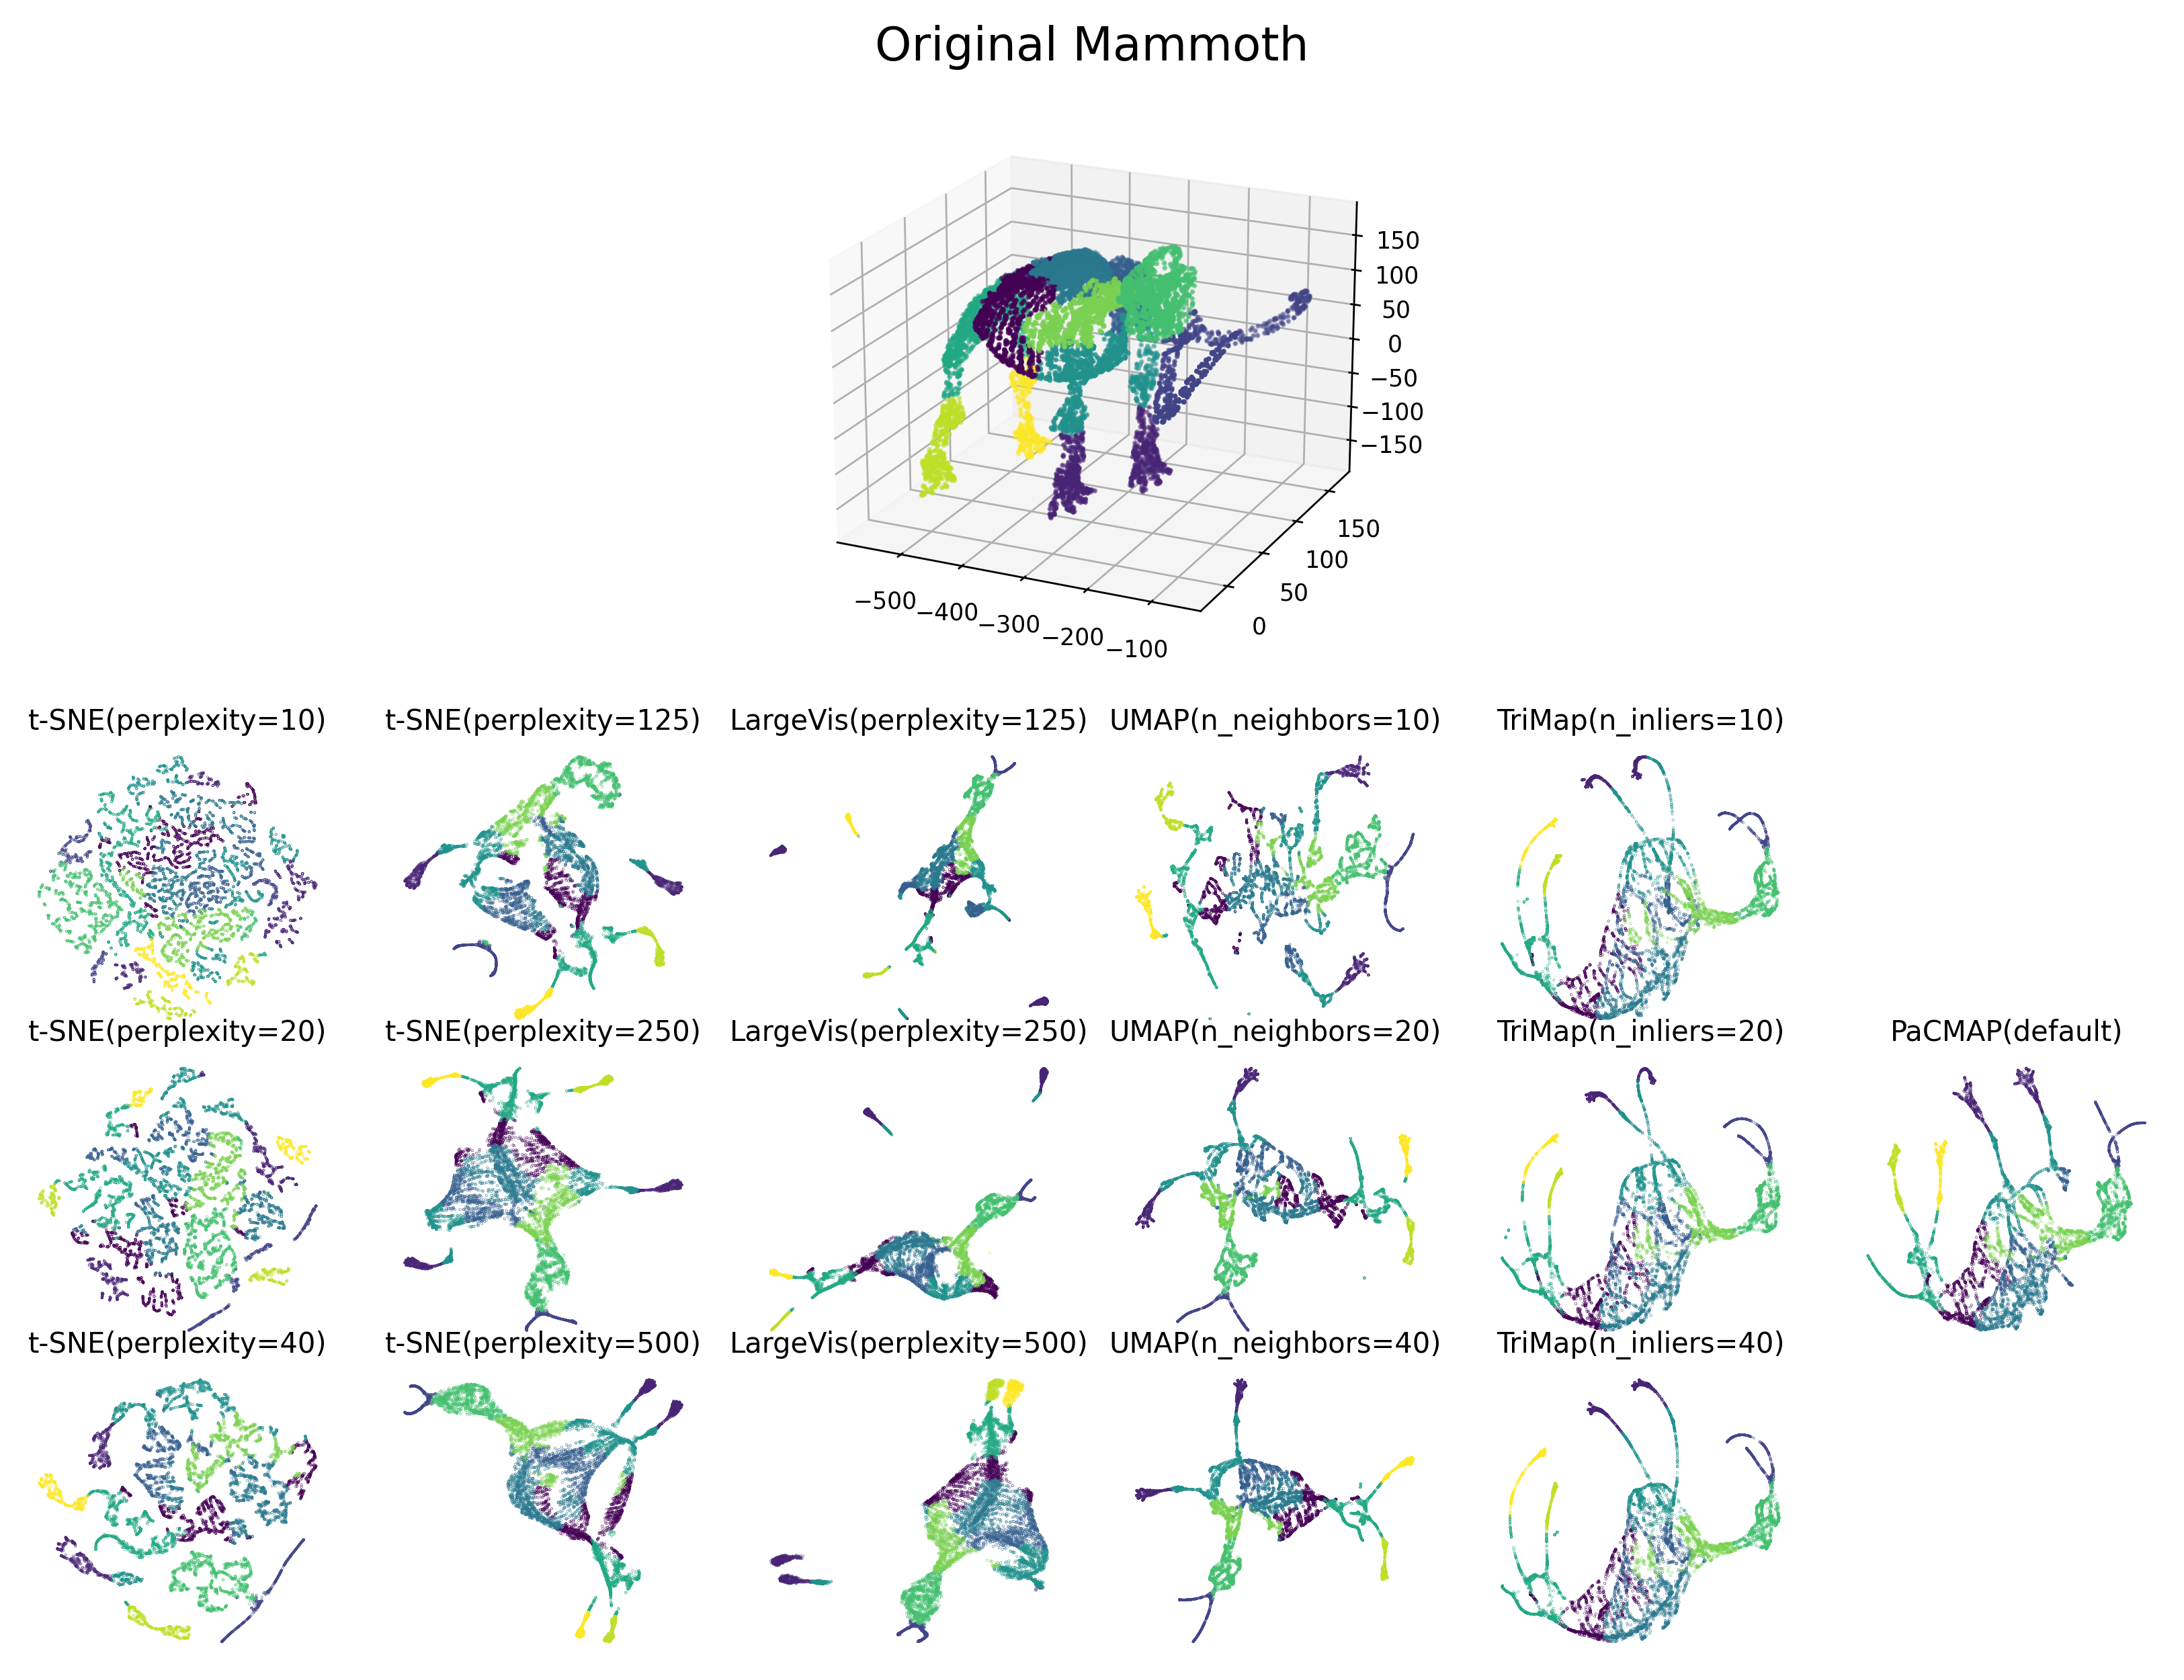
\includegraphics[width=0.95\columnwidth]{figures/Mammoth_21_3}
		\caption{Application of t-SNE, LargeVis, UMAP, TriMAP and PaCMAP to the Mammoth dataset, with their most important parameters shown. The preservation of local versus global structure is clear from looking at small details (such as the toes and tail of the mammoth) and the overall shape of the embedding.}
		\label{fig:Mammoth}
	\end{center}
\end{figure}
%----------------------------------------------------------------------------
\chapter{Resources}\label{ch:resources}
%----------------------------------------------------------------------------

In order to effectively explore the differences between the previously described algorithms, I needed a sufficiently large dataset and computational resources. In this chapter, I will describe the data on which I used these algorithms and the hardware resources I utilised to run said the clusterings.

\section{Used data}\label{sec:used-data}

The data I used was the latent representation of more than 1.6 million unique SMILES strings \cite{bib:smiles}. These strings were collected from two databases and served as an input to a variational autoencoder in order to embed them into a 64 dimensional latent representation, that preserved some of the chemical structure from the kernel space to the image \cite{bib:thesis}. If this preservation of chemical structure exists, we should find that after running the previously described algorithms, the resulting two dimensional space also has a smoothness over chemical structure.

The dataset had more features than the SMILES and latent representation of the molecules. Certain chemical descriptors, such as \textit{quantitative estimate of drug-likeness} (qed \cite{bib:qed}), \textit{synthetic accessibility score} (SaS \cite{bib:sas}) among many others. Overall, seven such chemical descriptors were included in the database along with one feature to indicate the database of origin of the string. The last feature was an indicator of the whether the data point was in the test set or not during the training of the model. These features -- with the exception of the last two -- were all factored into the loss function of the model, so the latent space should be relatively smooth over these values.

\section{Hardware resources}\label{sec:hardware-resources}

In terms of hardware, the requirements were quite beyond a standard personal computer's specification. Fortunately, I was granted access to a department server called Phoenix. This computer has 12 processing cores and 64 GB of RAM. In terms of GPU resources, it has an nVidia TITAN Xp graphics card, which I was able to use for running a t-SNE implementation to drastically reduce the runtime of the algorithm.

At the end of the semester, I was granted access to another department computer, called Nyx, which has 48 processing units and 250 GB of RAM and also has an nVidia TITAN Xp. I did not use this server in the end, since by the time I got access to it, the development phase of the project was nearly completed, however, I plan to utilise it in the future for the continuation of the project.

\section{Software resources}\label{sec:software-resources}

The first decision I had to make was the development environment. The most reasonable approach was developing in Python. This is due to the ease of development and the abundance of scientific packages, including at least one implementation of all five of the studied algorithms. 

For the reading, processing and writing of data, used the \texttt{numpy} and \texttt{pandas} libraries. For visualizing embedded latent spaces, \texttt{matplotlib} was used. The chemical computations were performed by \texttt{RDKit}\cite{bib:rdkit}.

For the PCA algorithm, I used the \texttt{scikit-learn==0.24.1} implementation. Two t-SNE implementation was used, \texttt{openTSNE==0.6.1} is a versatile CPU-based package, and \texttt{tsnecuda==3.0.0} is one with GPU utilization capabilities. The UMAP implementation I used was \texttt{umap-learn==0.5.2}. The TriMAP implementation was \texttt{trimap==1.0.15}. Finally, for PaCMAP, I used the package \texttt{pacmap==0.5.3}.
%----------------------------------------------------------------------------
\chapter{Own work}\label{ch:own-work}
%----------------------------------------------------------------------------

In this chapter, I will describe my work, from the specification of the task through the testing process to the results. The structuring of the experiments will mostly follow a chronological timeline, with the most basic questions answered first.

\section{Defining the objective}\label{sec:defining-the-objective}

The first problem I encountered during my work was that there is no clear definition of what a good embedding is. No simple metric exists that accurately and fully captures the nuances of embedding a latent chemical space in lower dimension. This is not surprising, since the very existence of so many different dimension algorithms comes from the fact that there is no consensus on that a good dimension reduction algorithm does. As such, I needed to define my own metrics for ranking each embedding. For this, I turned to the underlying goal of embedding these molecules.

The main objective of my thesis is exploring the capability of the previously described dimension reduction algorithms in novel drug discovery. Some assumptions must be made for formalizing the requirements. The first such assumption is that molecules that have similar a structure also have similar chemical properties. While this statement is not true for all chemical descriptors, it holds for most non-categorical metrics, such as number of rings in the molecule, or the topological polar surface area (TPSA~\cite{bib:tpsa}). This intuition implies that molecules with similar structure have similar binding properties to certain proteins too, which is the most vital metric for novel drug research. Drug molecules act by binding to proteins, forming complexes that induce physiological changes in the body. The efficacy of binding depends on the chemical properties of the target protein (mainly its three-dimensional shape) and the chemical properties of the drug molecule.

From this, it logically follows that a chemical space that is ordered over the chemical structure of molecules allows the targeted search of potential drug candidates. Unfortunately, chemical structure can not be quantized in such a way as to be able to order them. Instead, I decided that what I needed was a space that \textit{smooth} over chemical structure. In essence, this means that points close to each other have similar chemical structure. This is the exact property that is needed for targeted search. Importantly, this does not imply that points far away from each other have significantly different structure. Optimizing for embedding all similar molecules closely is a difficult task, and I can not be sure that points in the original 64-dimensional dataset even satisfies this condition. An algorithm that places all similarly structured molecules close together is advantageous, but for my purposes, not needed.

In summary, a good embedding is one that is locally smooth over chemical structure. This can most easily be determined by looking at chemical descriptors of molecules, and assessing their local smoothness in the output space.

The choice of descriptors matters greatly in this question. The original model was trained on millions of molecules, and some of their chemical properties. The properties used by the VAE's property predictor was part of the database, which means that the 64-dimensional latent space should in theory be relatively smooth over those metrics. Because of this, the inclusion of other chemical descriptors are needed for a proper examination of data. With mostly smooth transitions on a large number of descriptors, one can be certain that the chemical structure itself changes smoothly.

\section{Initial testing}\label{sec:initial-testing}

After defining the objective, the first thing that I did was running each algorithm with default parametrization to see baseline results. This served two purposes. Firstly, by generating baseline embeddings, the effect of different parametrization could be more accurately assessed. Secondly, I recorded the runtime of each algorithm, so their performance could be compared from a different angle.

After running each algorithm once, I noticed that the t-SNE clustering was somewhat strange (as can be seen on figure (\ref{fig:default_run})). The result of this run did not make much sense. It was completely different from what I expected. I had prior experience using t-SNE, albeit another implementation. After rerunning the algorithm, I found a similar result, which led me to believe that the implementation had some bug. Indeed, when I ran t-SNE again in verbose mode, I found that instead of the 2000 iterations specified, it only ran for about 150, which was not enough to form proper clusters. I tried switching to openTSNE, the implementation I used heavily during my project laboratory, however, the sheer size of the dataset made it unusable as the system did not have enough memory to accommodate its needs.

\begin{figure}[!ht]
	\centering
	\includegraphics[width=0.49\columnwidth, keepaspectratio]{figures/PCA_default}
	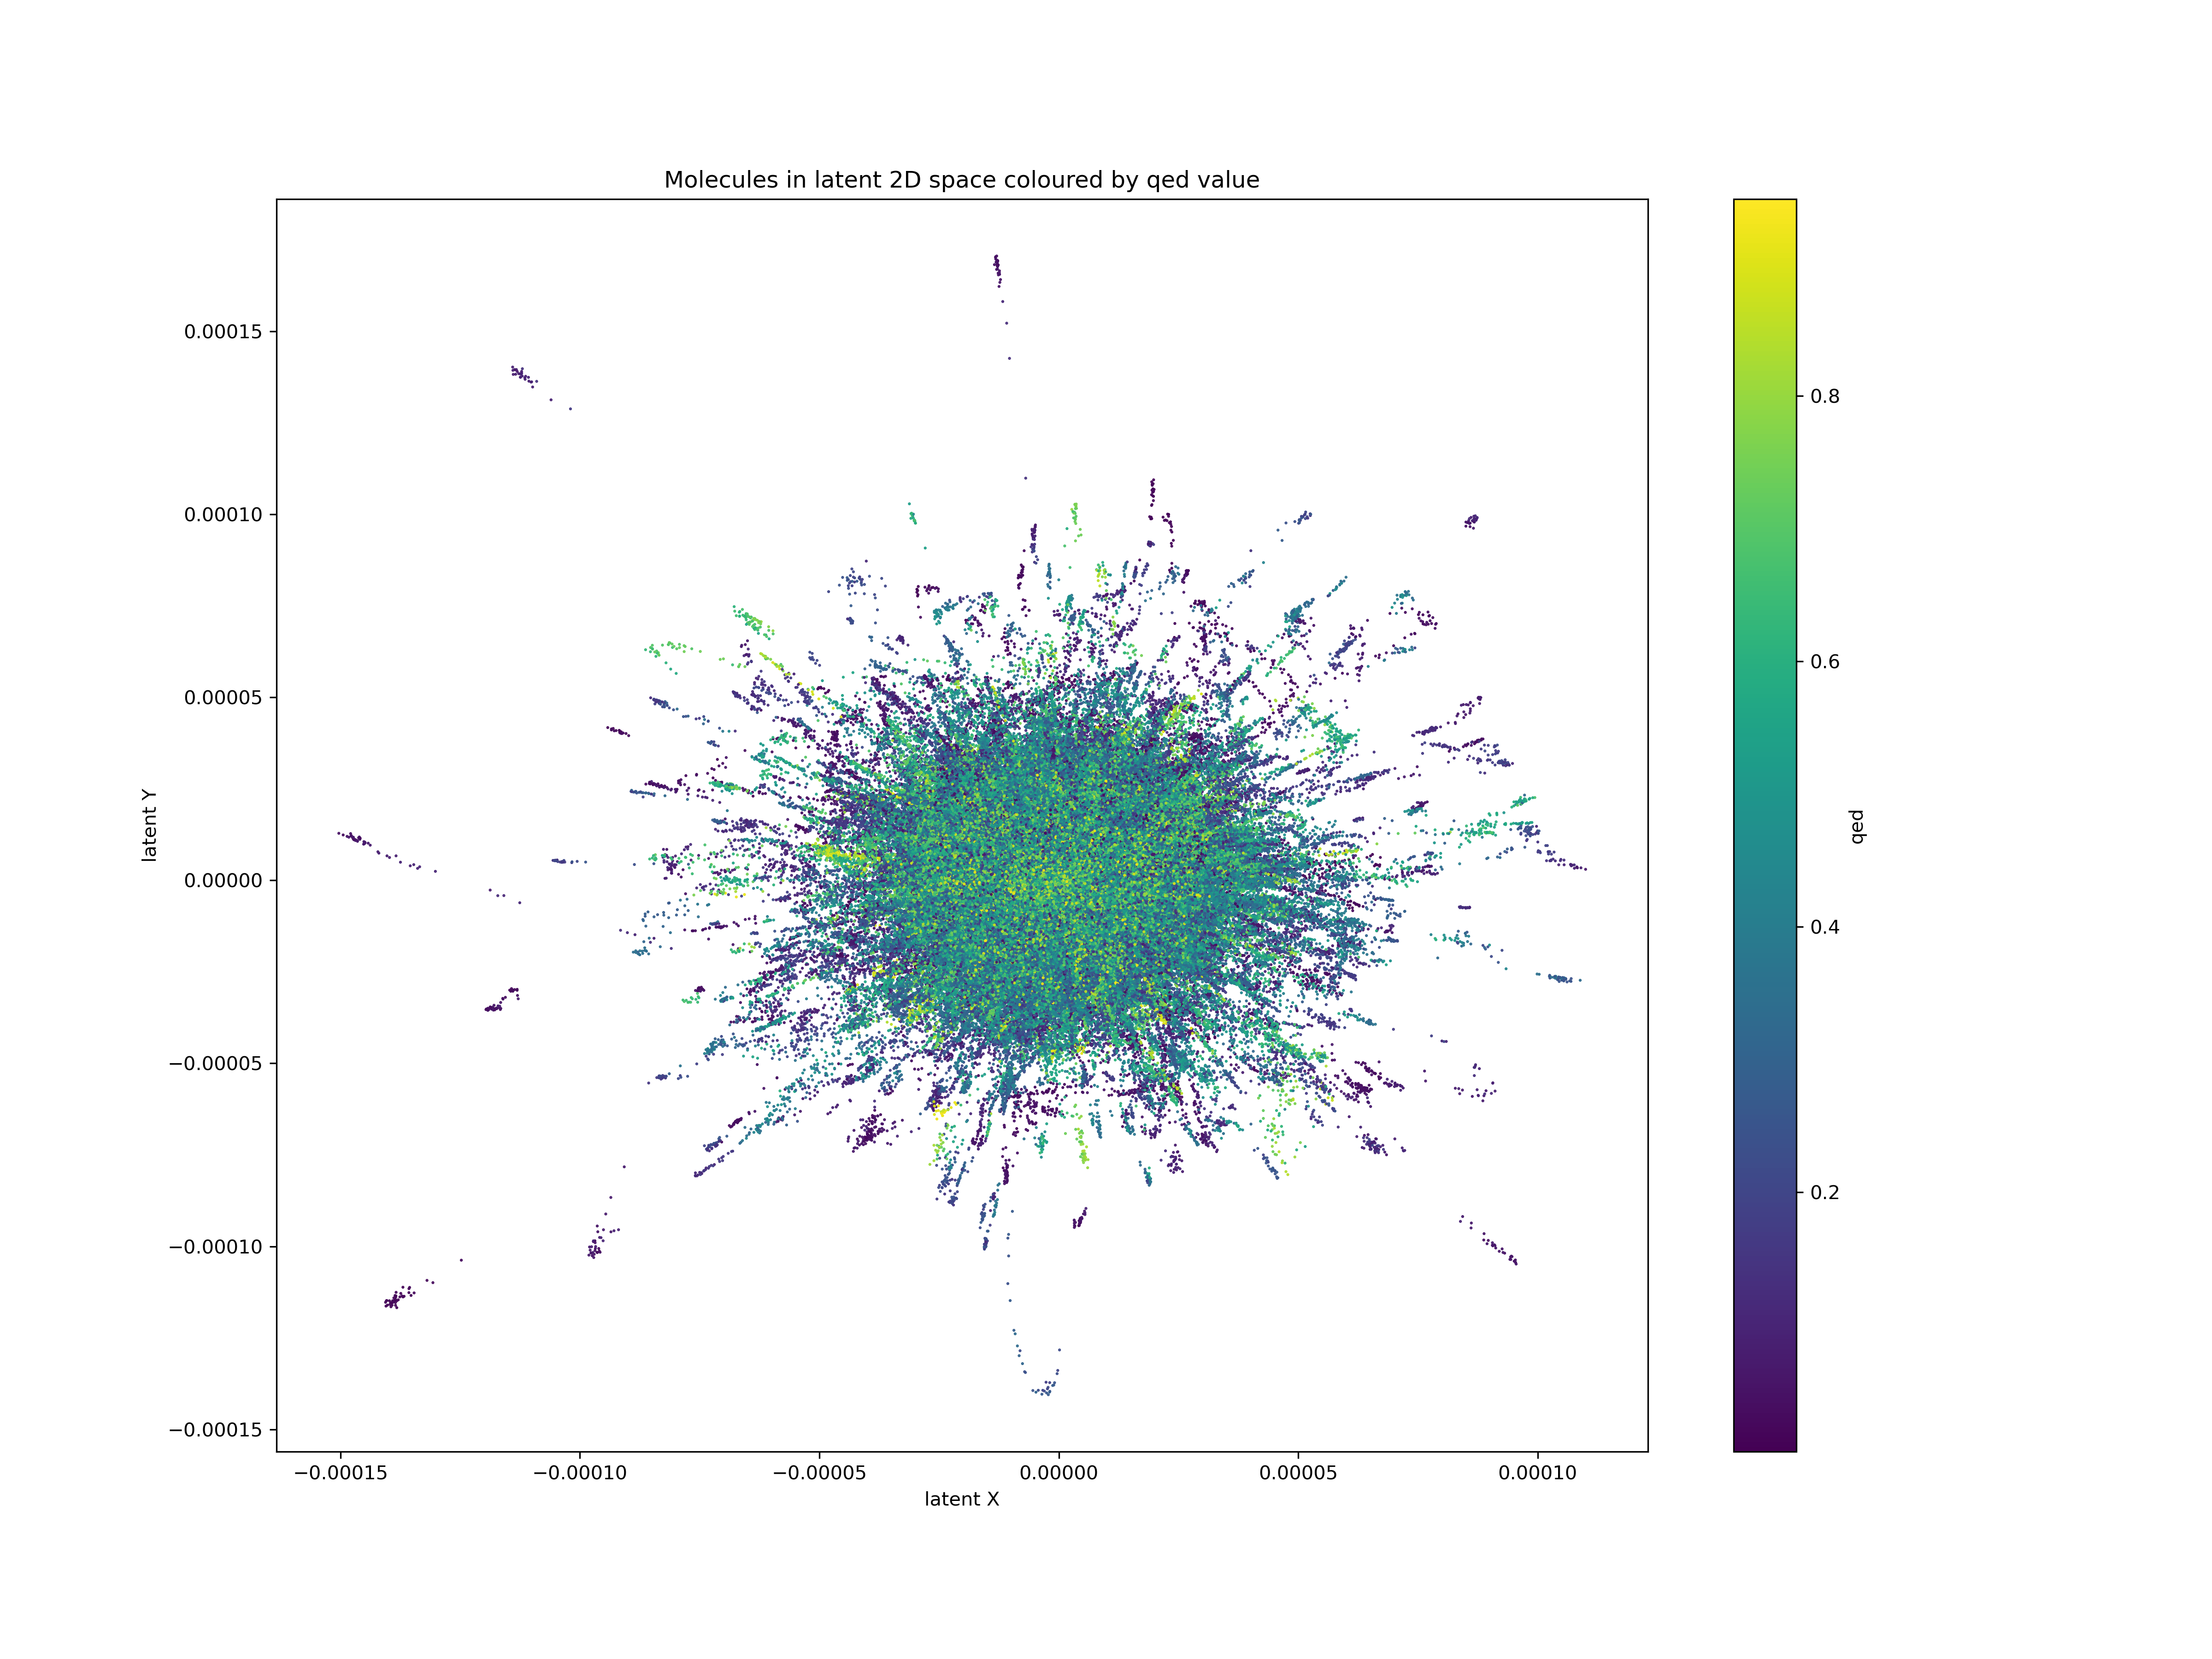
\includegraphics[width=0.49\columnwidth, keepaspectratio]{figures/t-SNE_default}
	\includegraphics[width=0.49\columnwidth, keepaspectratio]{figures/t-SNE2_default}
	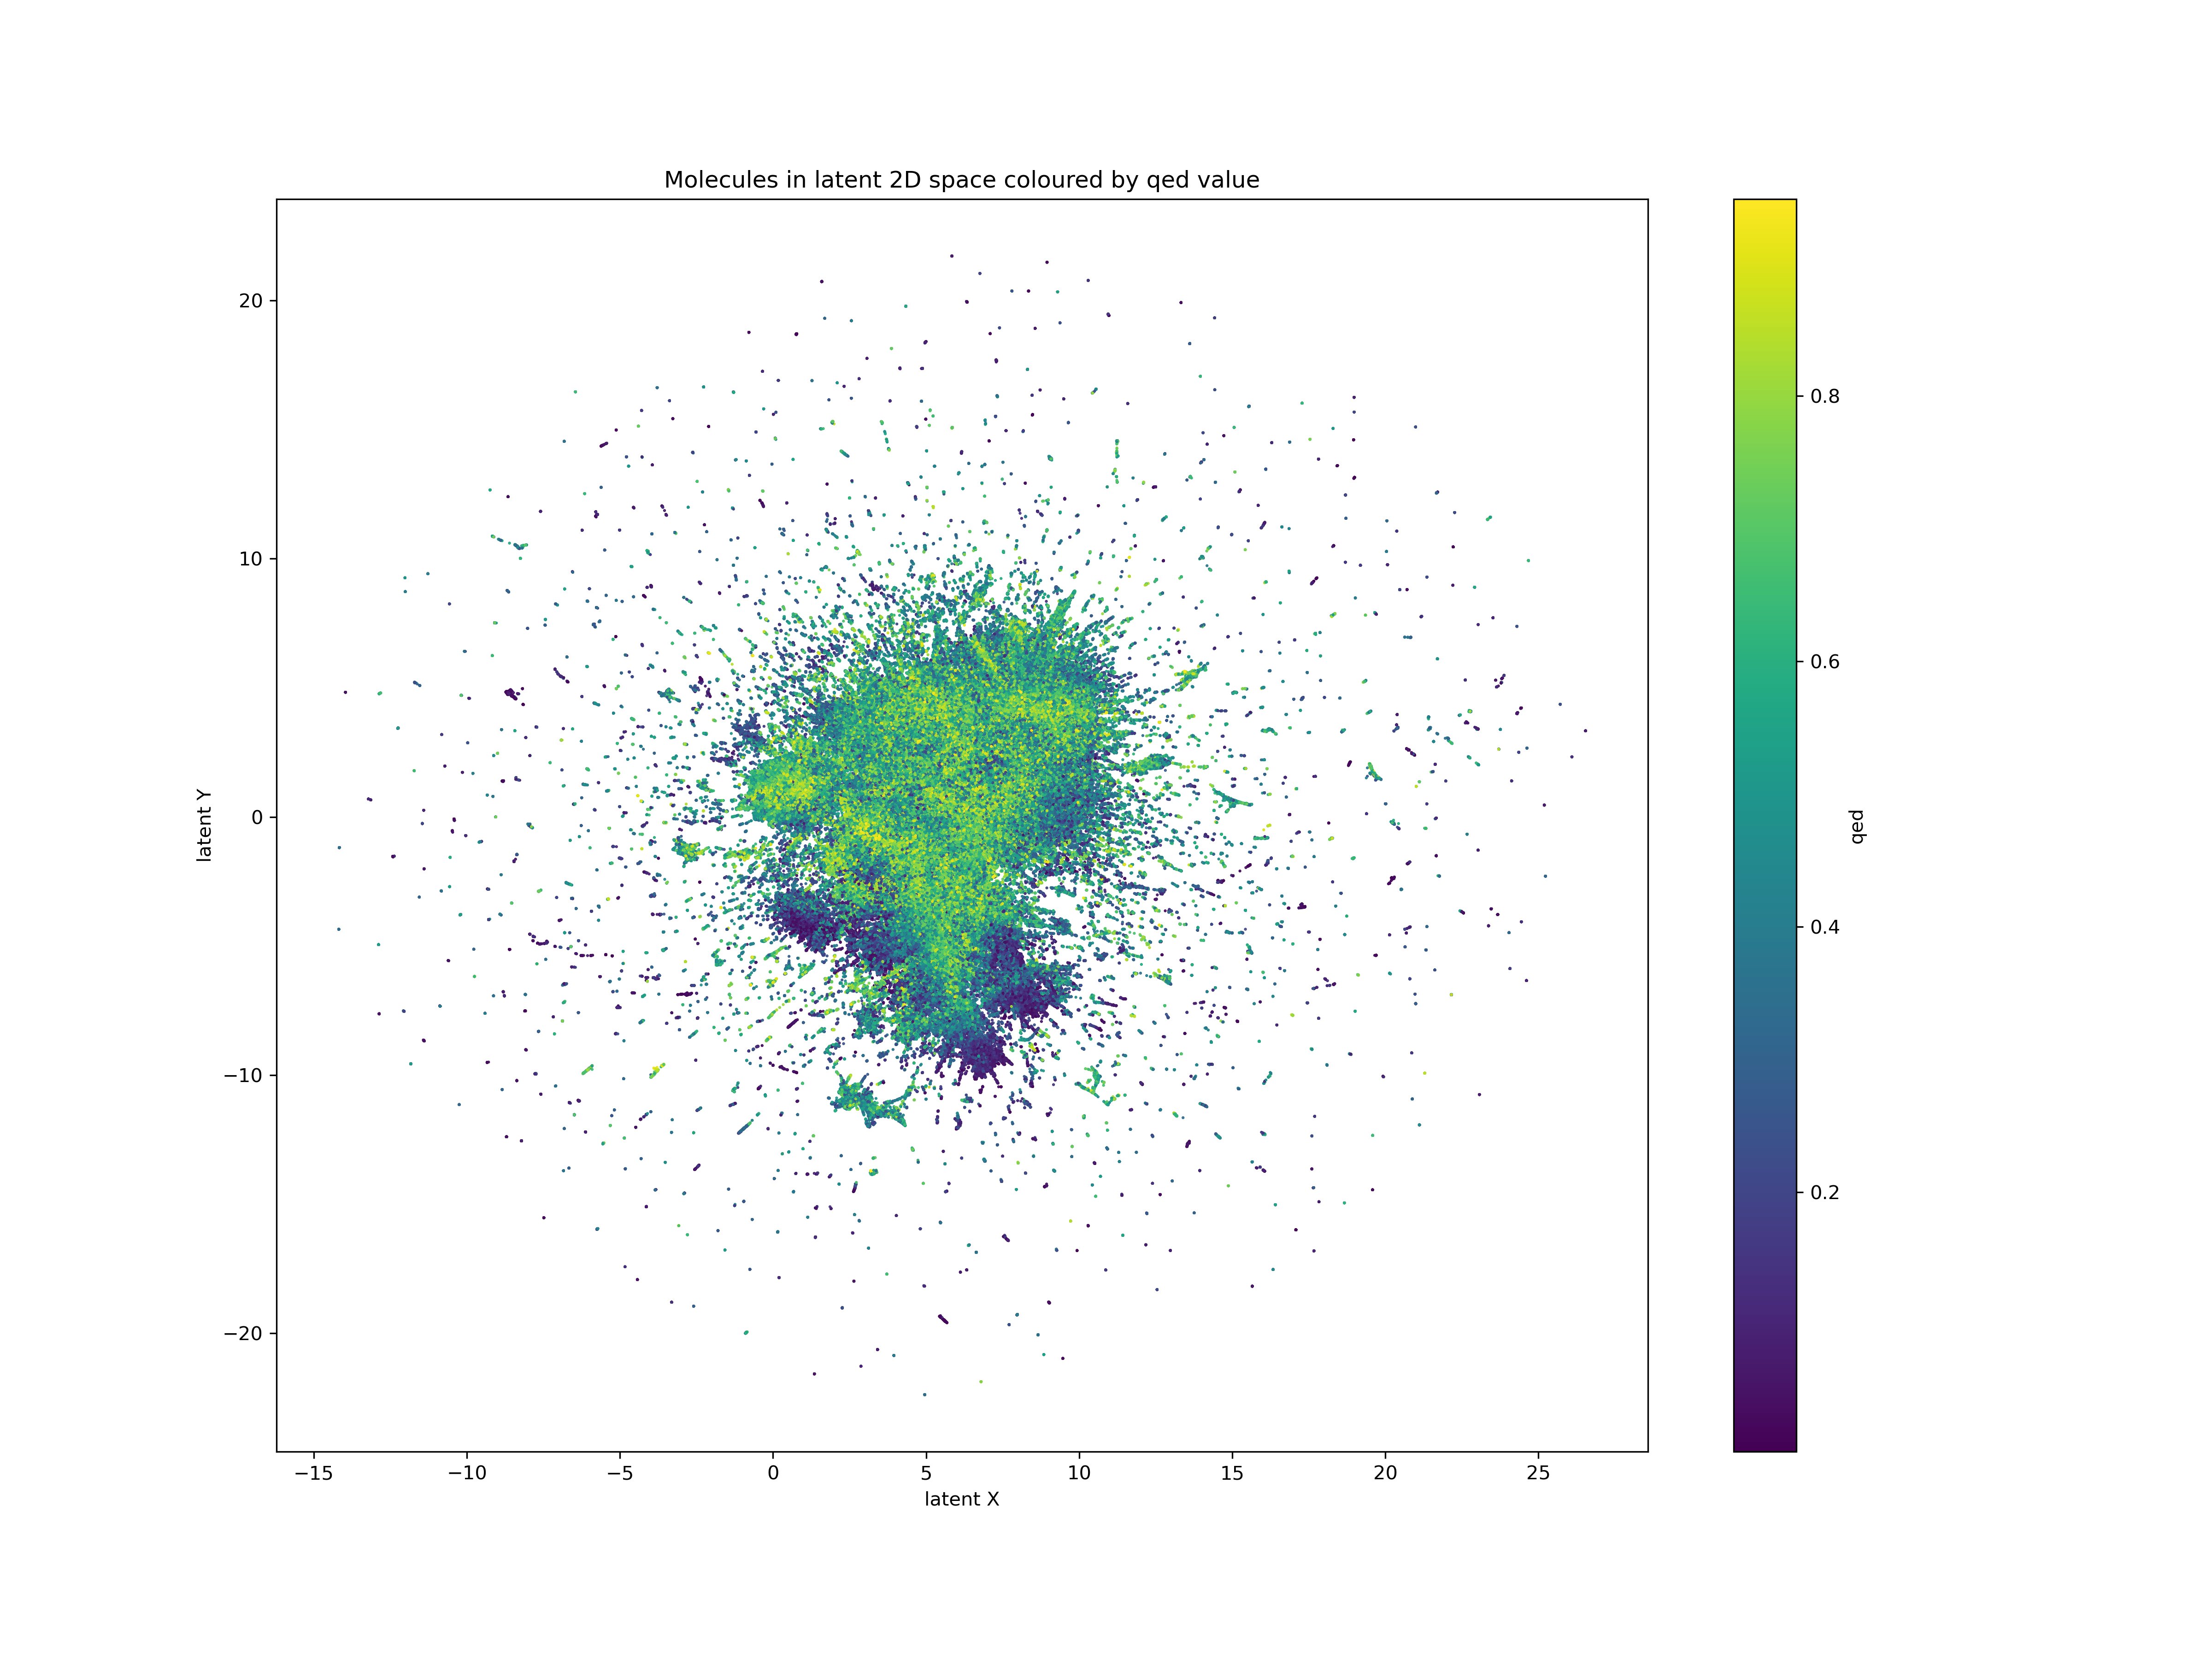
\includegraphics[width=0.49\columnwidth, keepaspectratio]{figures/UMAP_default}
	\includegraphics[width=0.49\columnwidth, keepaspectratio]{figures/TriMAP_default}
	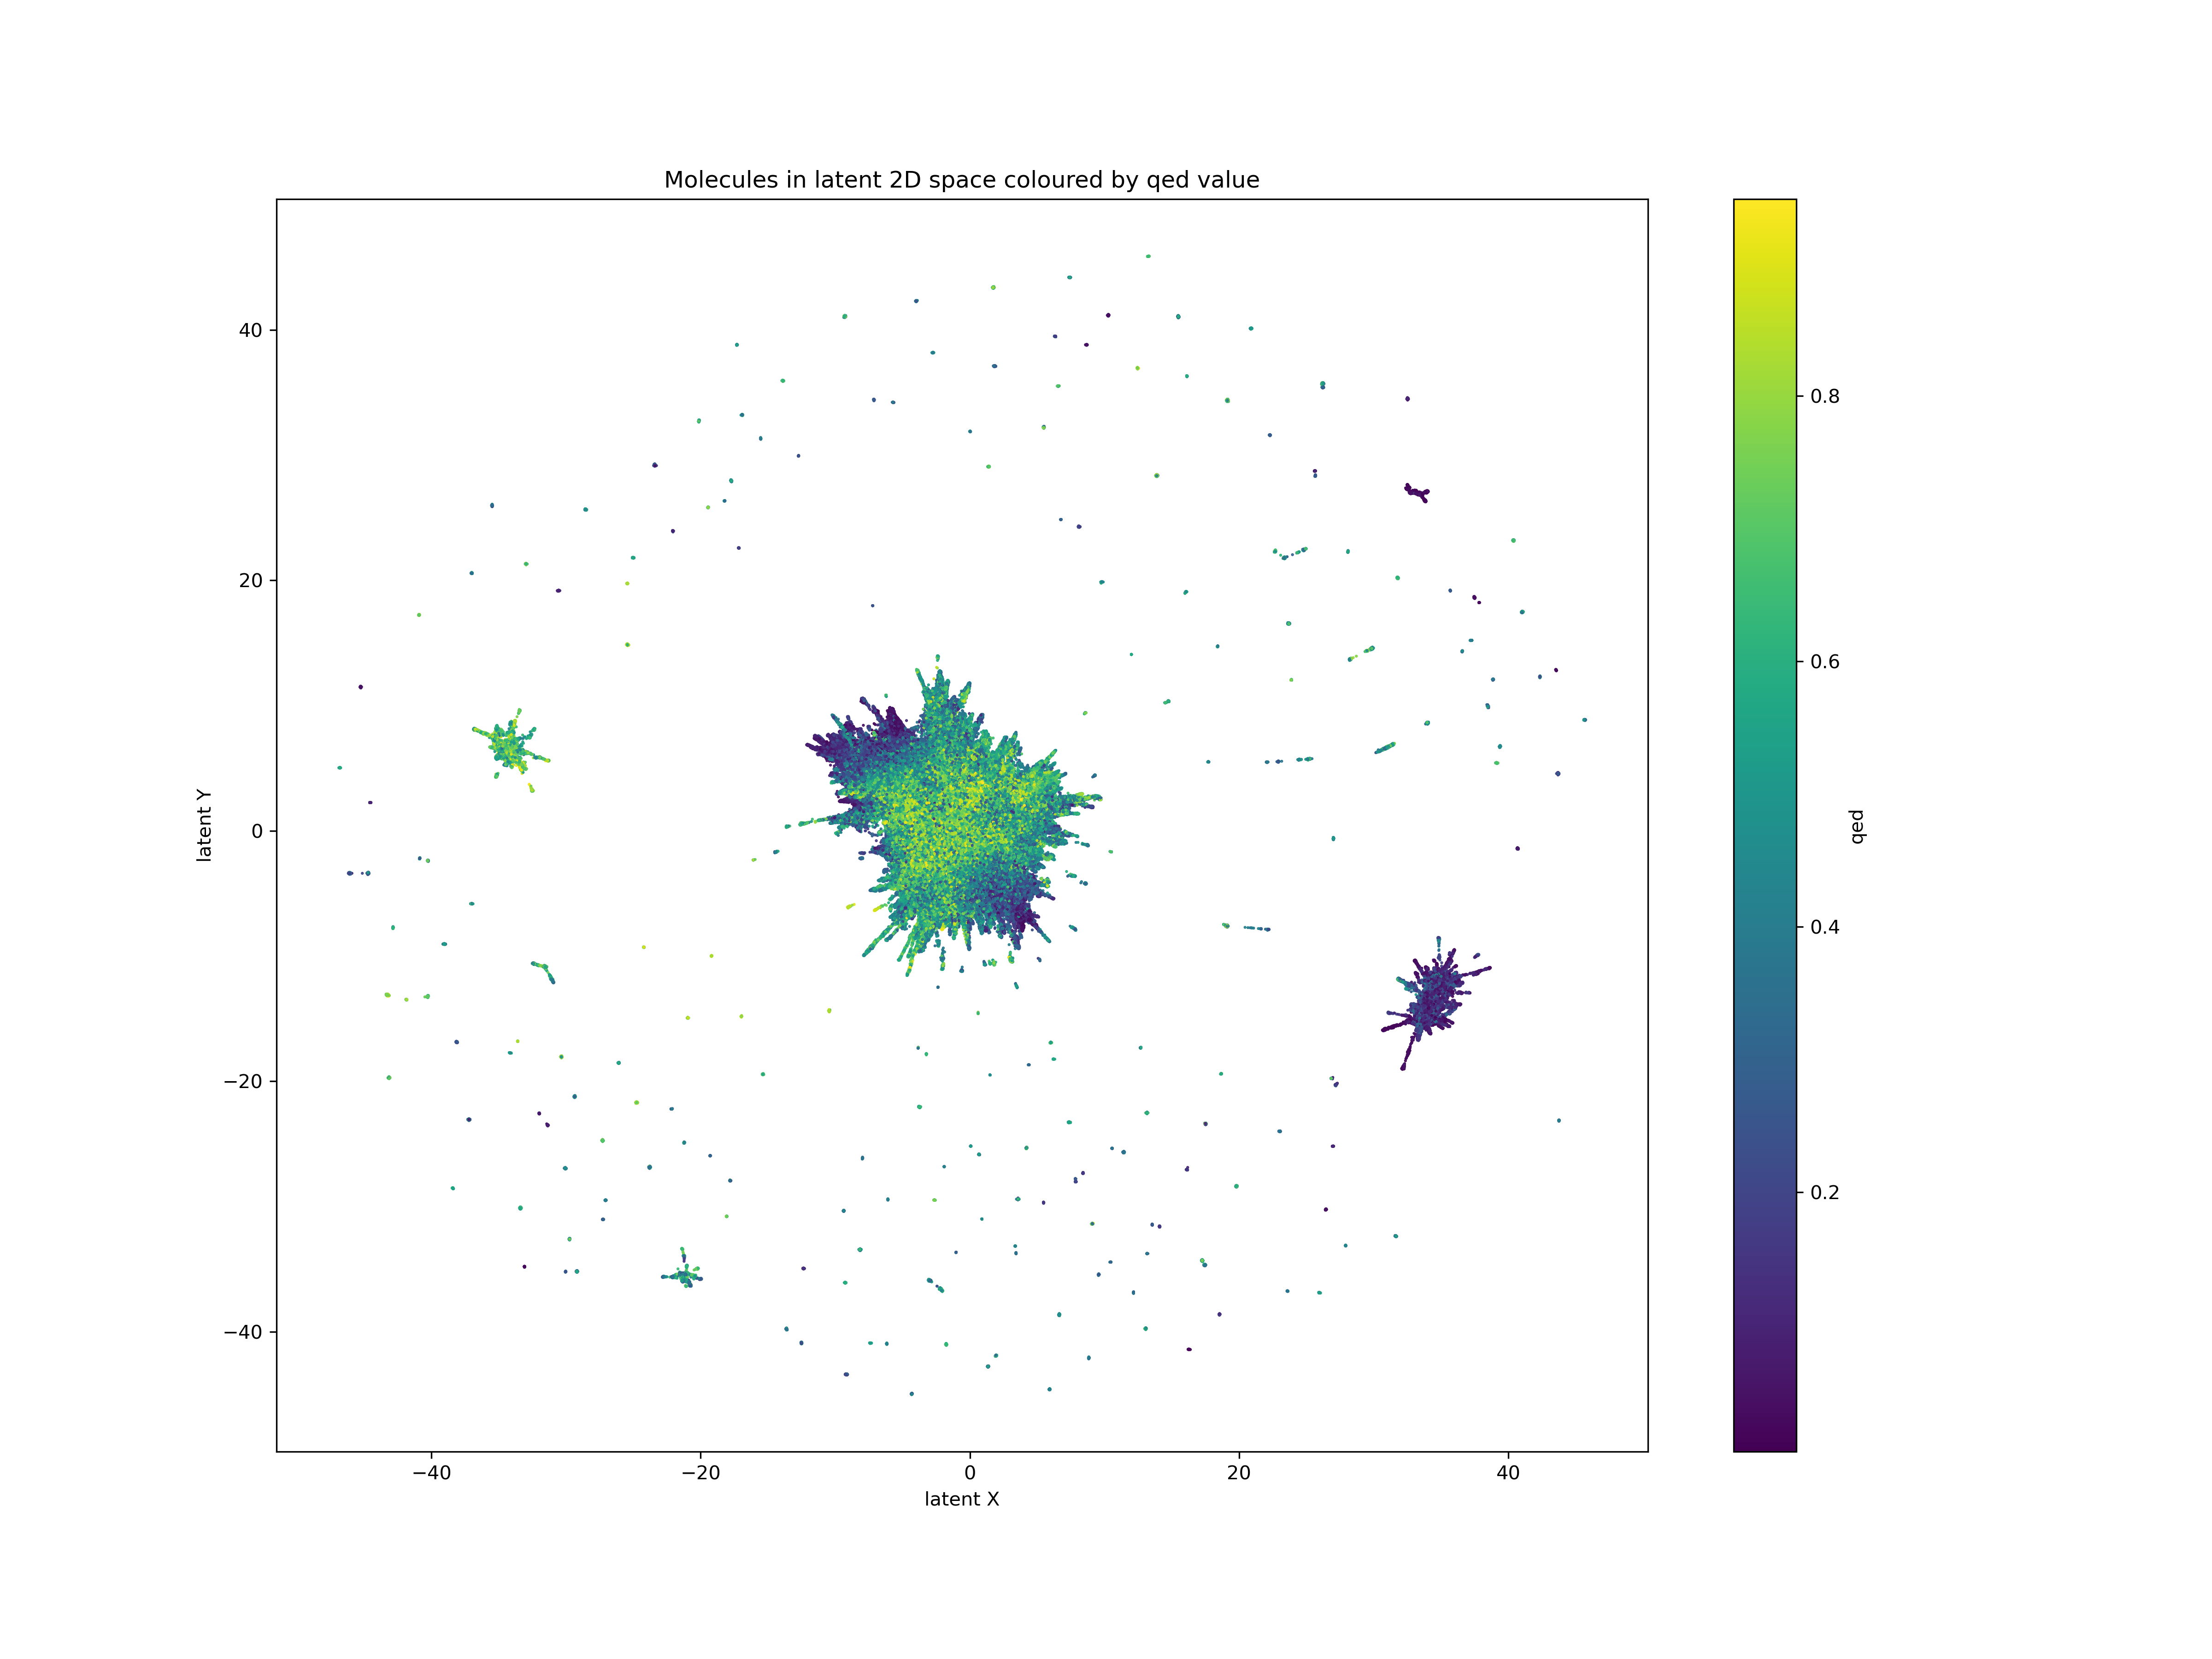
\includegraphics[width=0.49\columnwidth, keepaspectratio]{figures/PaCMAP_default}
	\caption{Results of PCA, t-SNE (sklearn and tsnecuda), UMAP, TriMAP and PaCMAP algorithms on the dataset with default parameters, coloured by the quantitative estimate of drug-likeness of each data point. It can be clearly seen that each algorithm places points very differently.}
	\label{fig:default_run}
\end{figure}

After some consideration, I turned to tsnecuda, another familiar implementation that ran on the GPU (and as such, used its own memory instead of the RAM of the system). I initially chose openTSNE for two reasons: firstly, it was more usable that tsnecuda, as it was far more parametrizable, allowing for custom callback functions and deterministic runs. Secondly, all other algorithm ran on the CPU, making performance comparisons more fair with openTSNE. Since openTSNE could not even complete one run, I was forced to use tsnecuda. This switch however highlighted something very interesting.

In the field of deep learning, GPU's are widely used as they are capable of running thousands of operations in parallel, leading to faster training of models. All graph-based clustering algorithms work very similarly to a neural network, in that they exclusively work with matrices and are highly parallelizable. This means that using GPU resources can significantly speed up the clustering of any given dataset. As can be seen on table (\ref{tab:runtime}), while the sklearn t-SNE implementation took almost exactly 25 hours to run for 150 iterations (plus constructing the higher dimensional probability distribution), tsnecuda did not even take six minutes to perform 5000 iterations (in fact, in the first run, I set it to only 2000 iterations, which ran for 102 seconds, an incredible 883 times faster).

\begin{table}[htb]
	\begin{center}
		\begin{tabular}{|l|r|}
			\hline
			Algorithm (iterations) & runtime \\
			\hline
			PCA & 19.45 s \\
			\hline
			t-SNE (sklearn, 150) & 90 042 s \\
			\hline
			t-SNE (tsnecuda, 5000) & 344.29 s \\
			\hline
			UMAP (1000 epochs) & 5 866.55 s \\
			\hline
			TriMAP (2000) & 26 756.64 s \\
			\hline
			PaCMAP (2000) & 65 283.52 s \\
			\hline
		\end{tabular}
	\end{center}
	\caption{Runtimes of each algorithm tested on the entire dataset (without duplicates, ~1.6 million molecules) given in seconds. The number of iterations and epochs are indicated where applicable. PCA, the only non-iterative method is the fastest, while the others take significantly more time. The power of GPU usage is clearly demonstrated by the two t-SNE implementations.}
	\label{tab:runtime}
\end{table}

Comparison of each algorithm based on the runtimes in table (\ref{tab:runtime}) should only be done in context. PCA is the fastest method of the bunch, this is because it is the only non-iterative algorithm. After that, the GPU implementation of t-SNE is the fastest, but this can not be credited to the algorithm, but the implementation instead. In fact, the slowest running algorithm is also a t-SNE implementation, which ran on the CPU. As for the other graph-based algorithms, they are not equal either. UMAP has multithreaded capabilities, while TriMAP and PaCMAP do not.

In summary, these runtime metrics are not intrinsic properties of the algorithms. They merely describe the performance of the current implementations. In time, more libraries will be available for every algorithm and these numbers will change. t-SNE and UMAP both have GPU implementations which vastly outperform their CPU implementations, and even other algorithms that are supposed to be faster than them. In an engineering application, it is important to consider technical parameters, it should be noted that these parameters change as opposed to each algorithm's performance in terms of the quality of the embedding.

\section{Result of first runs}\label{sec:result-of-first-runs}

I have briefly touched on the importance of chemical descriptors in the inference of structure in section (\ref{sec:defining-the-objective}). Since the original model was trained with a property predictor, it is to be expected that the latent space is smooth over those descriptors. This can be seen on figure (\ref{fig:default_run}) with the quantitative estimate of drug-likeness (qed~\cite{bib:qed}). Additional metrics were needed to properly be able to induce chemical structure. This is needed because while structural similarity between molecules can easily be captured by one number, the structure of individual molecules is typically described by fingerprint vectors. These would form a vector space that is not easy to interpret.

\begin{figure}[!ht]
	\centering
	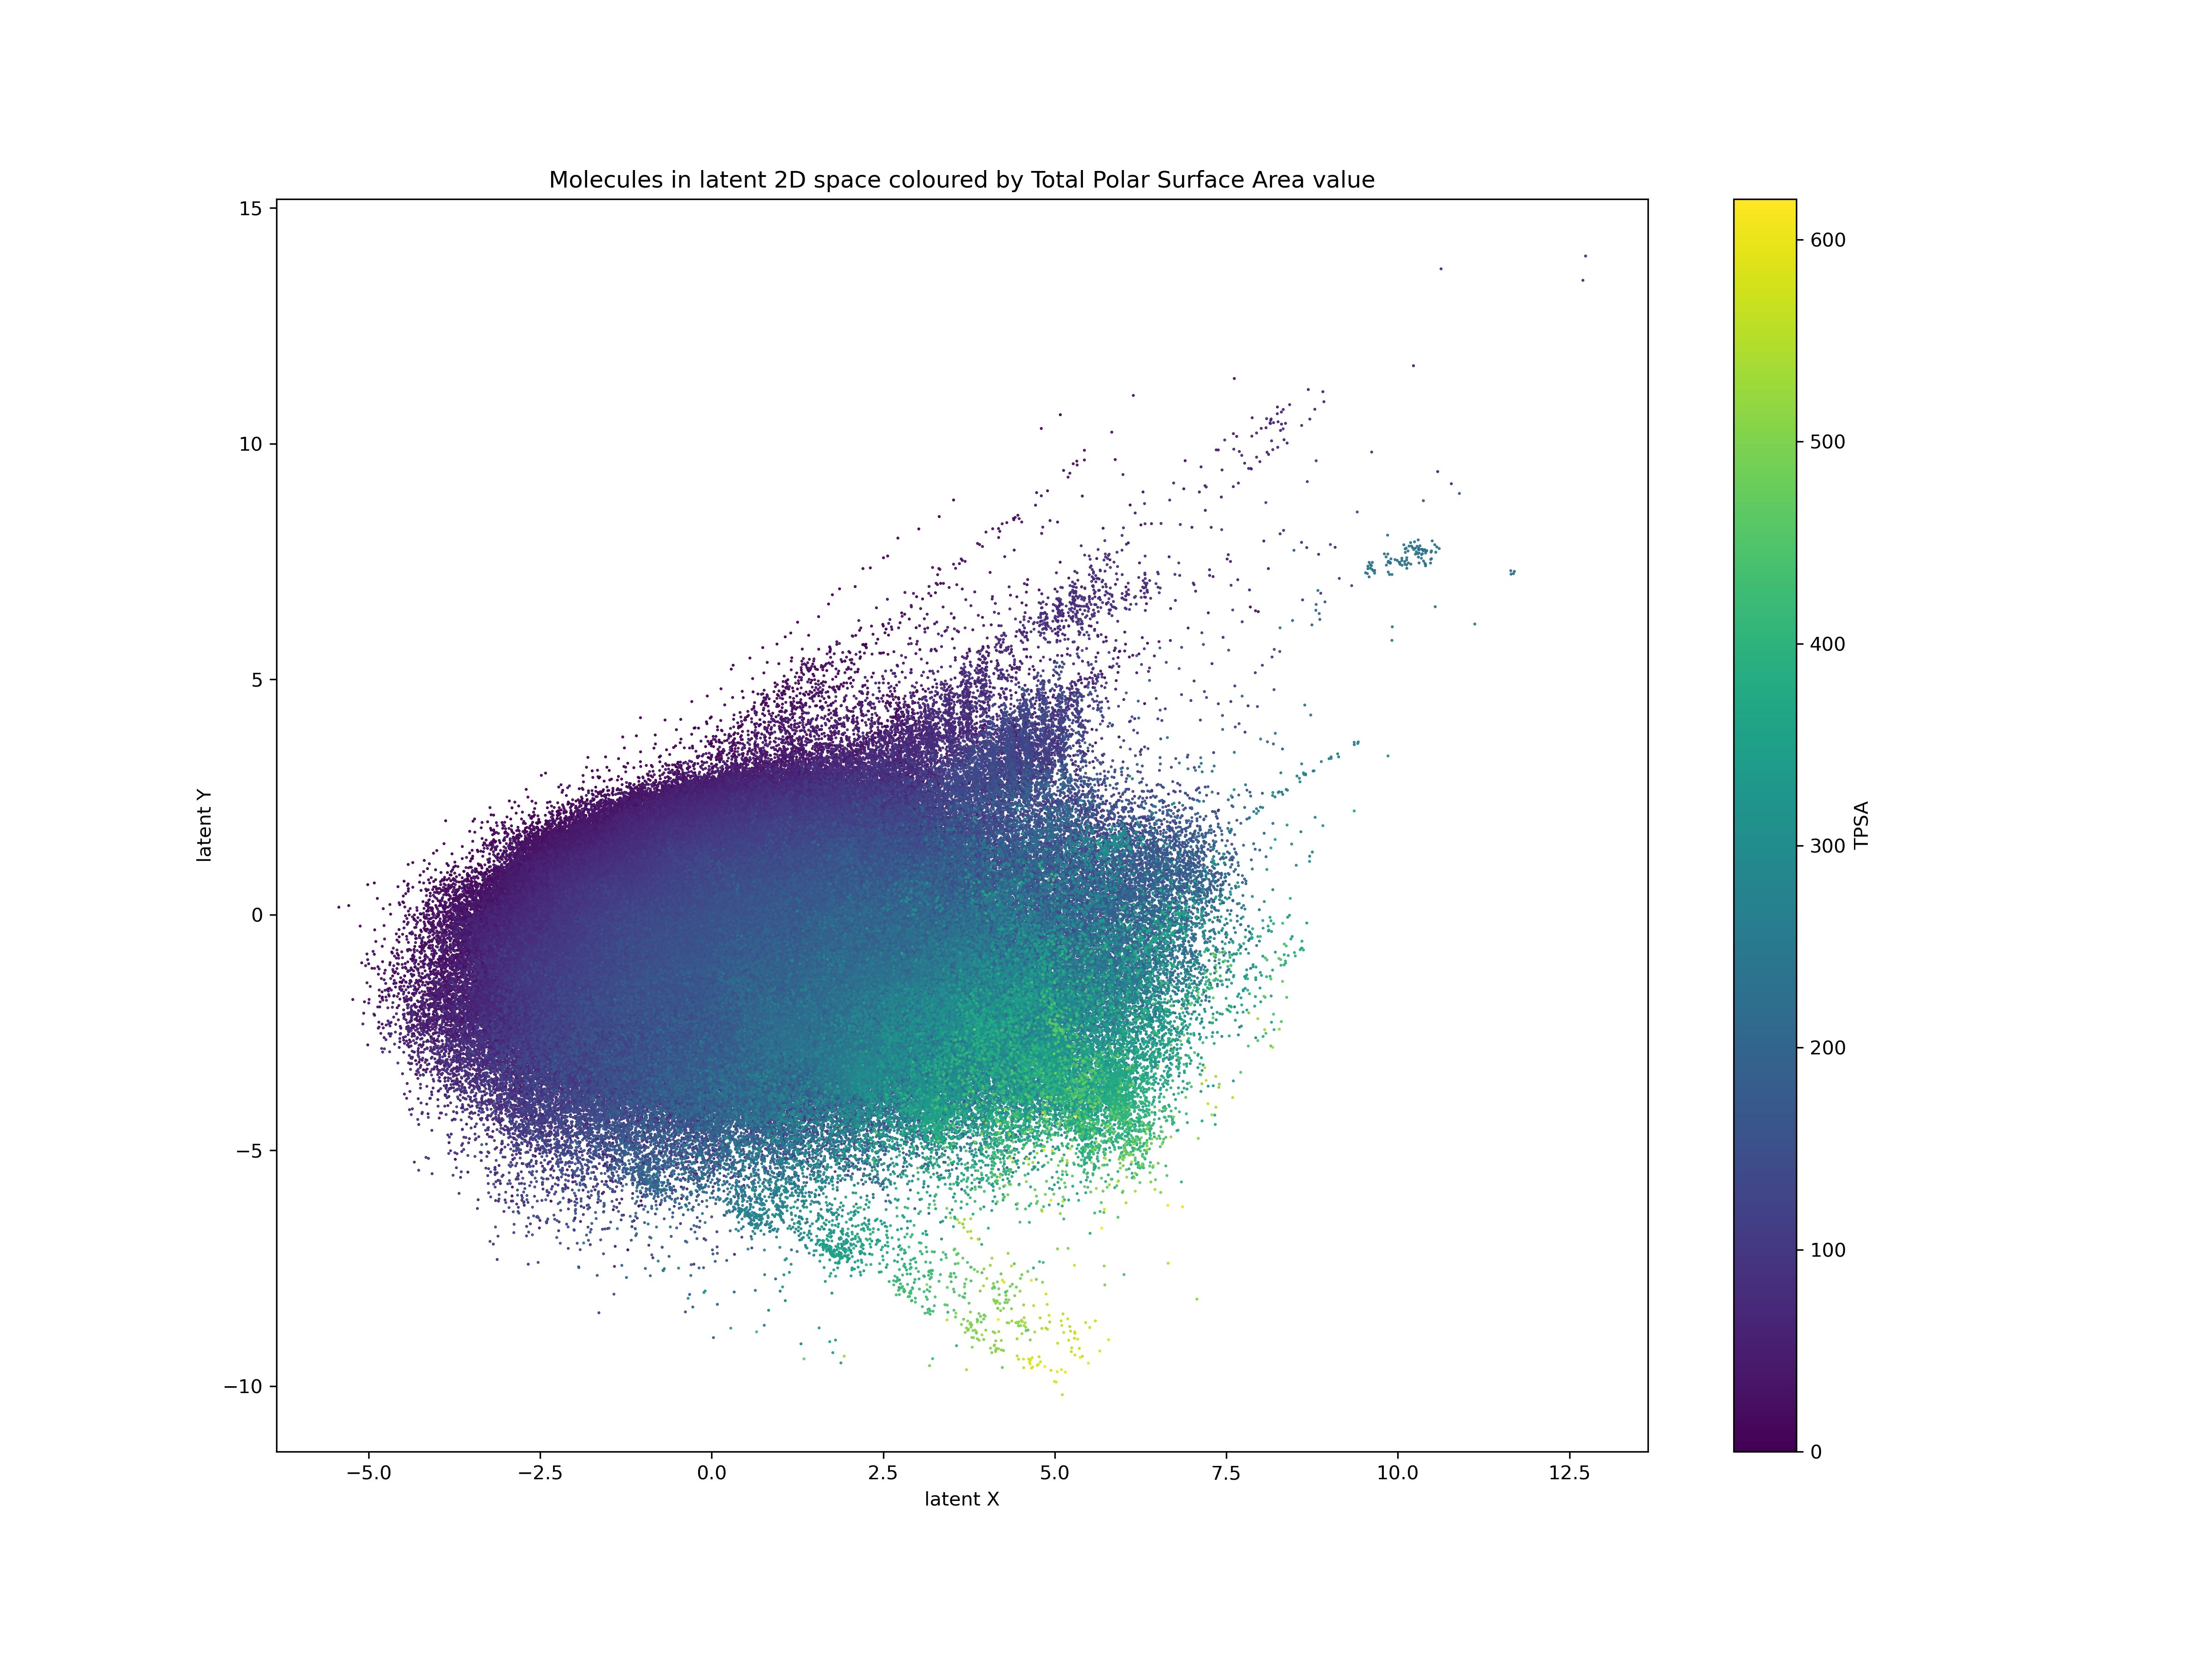
\includegraphics[width=0.49\columnwidth]{figures/TPSA_PCA}
	\includegraphics[width=0.49\columnwidth]{figures/TPSA_t-SNE}
	\includegraphics[width=0.49\columnwidth]{figures/TPSA_UMAP}
	\includegraphics[width=0.49\columnwidth]{figures/TPSA_TriMAP}
	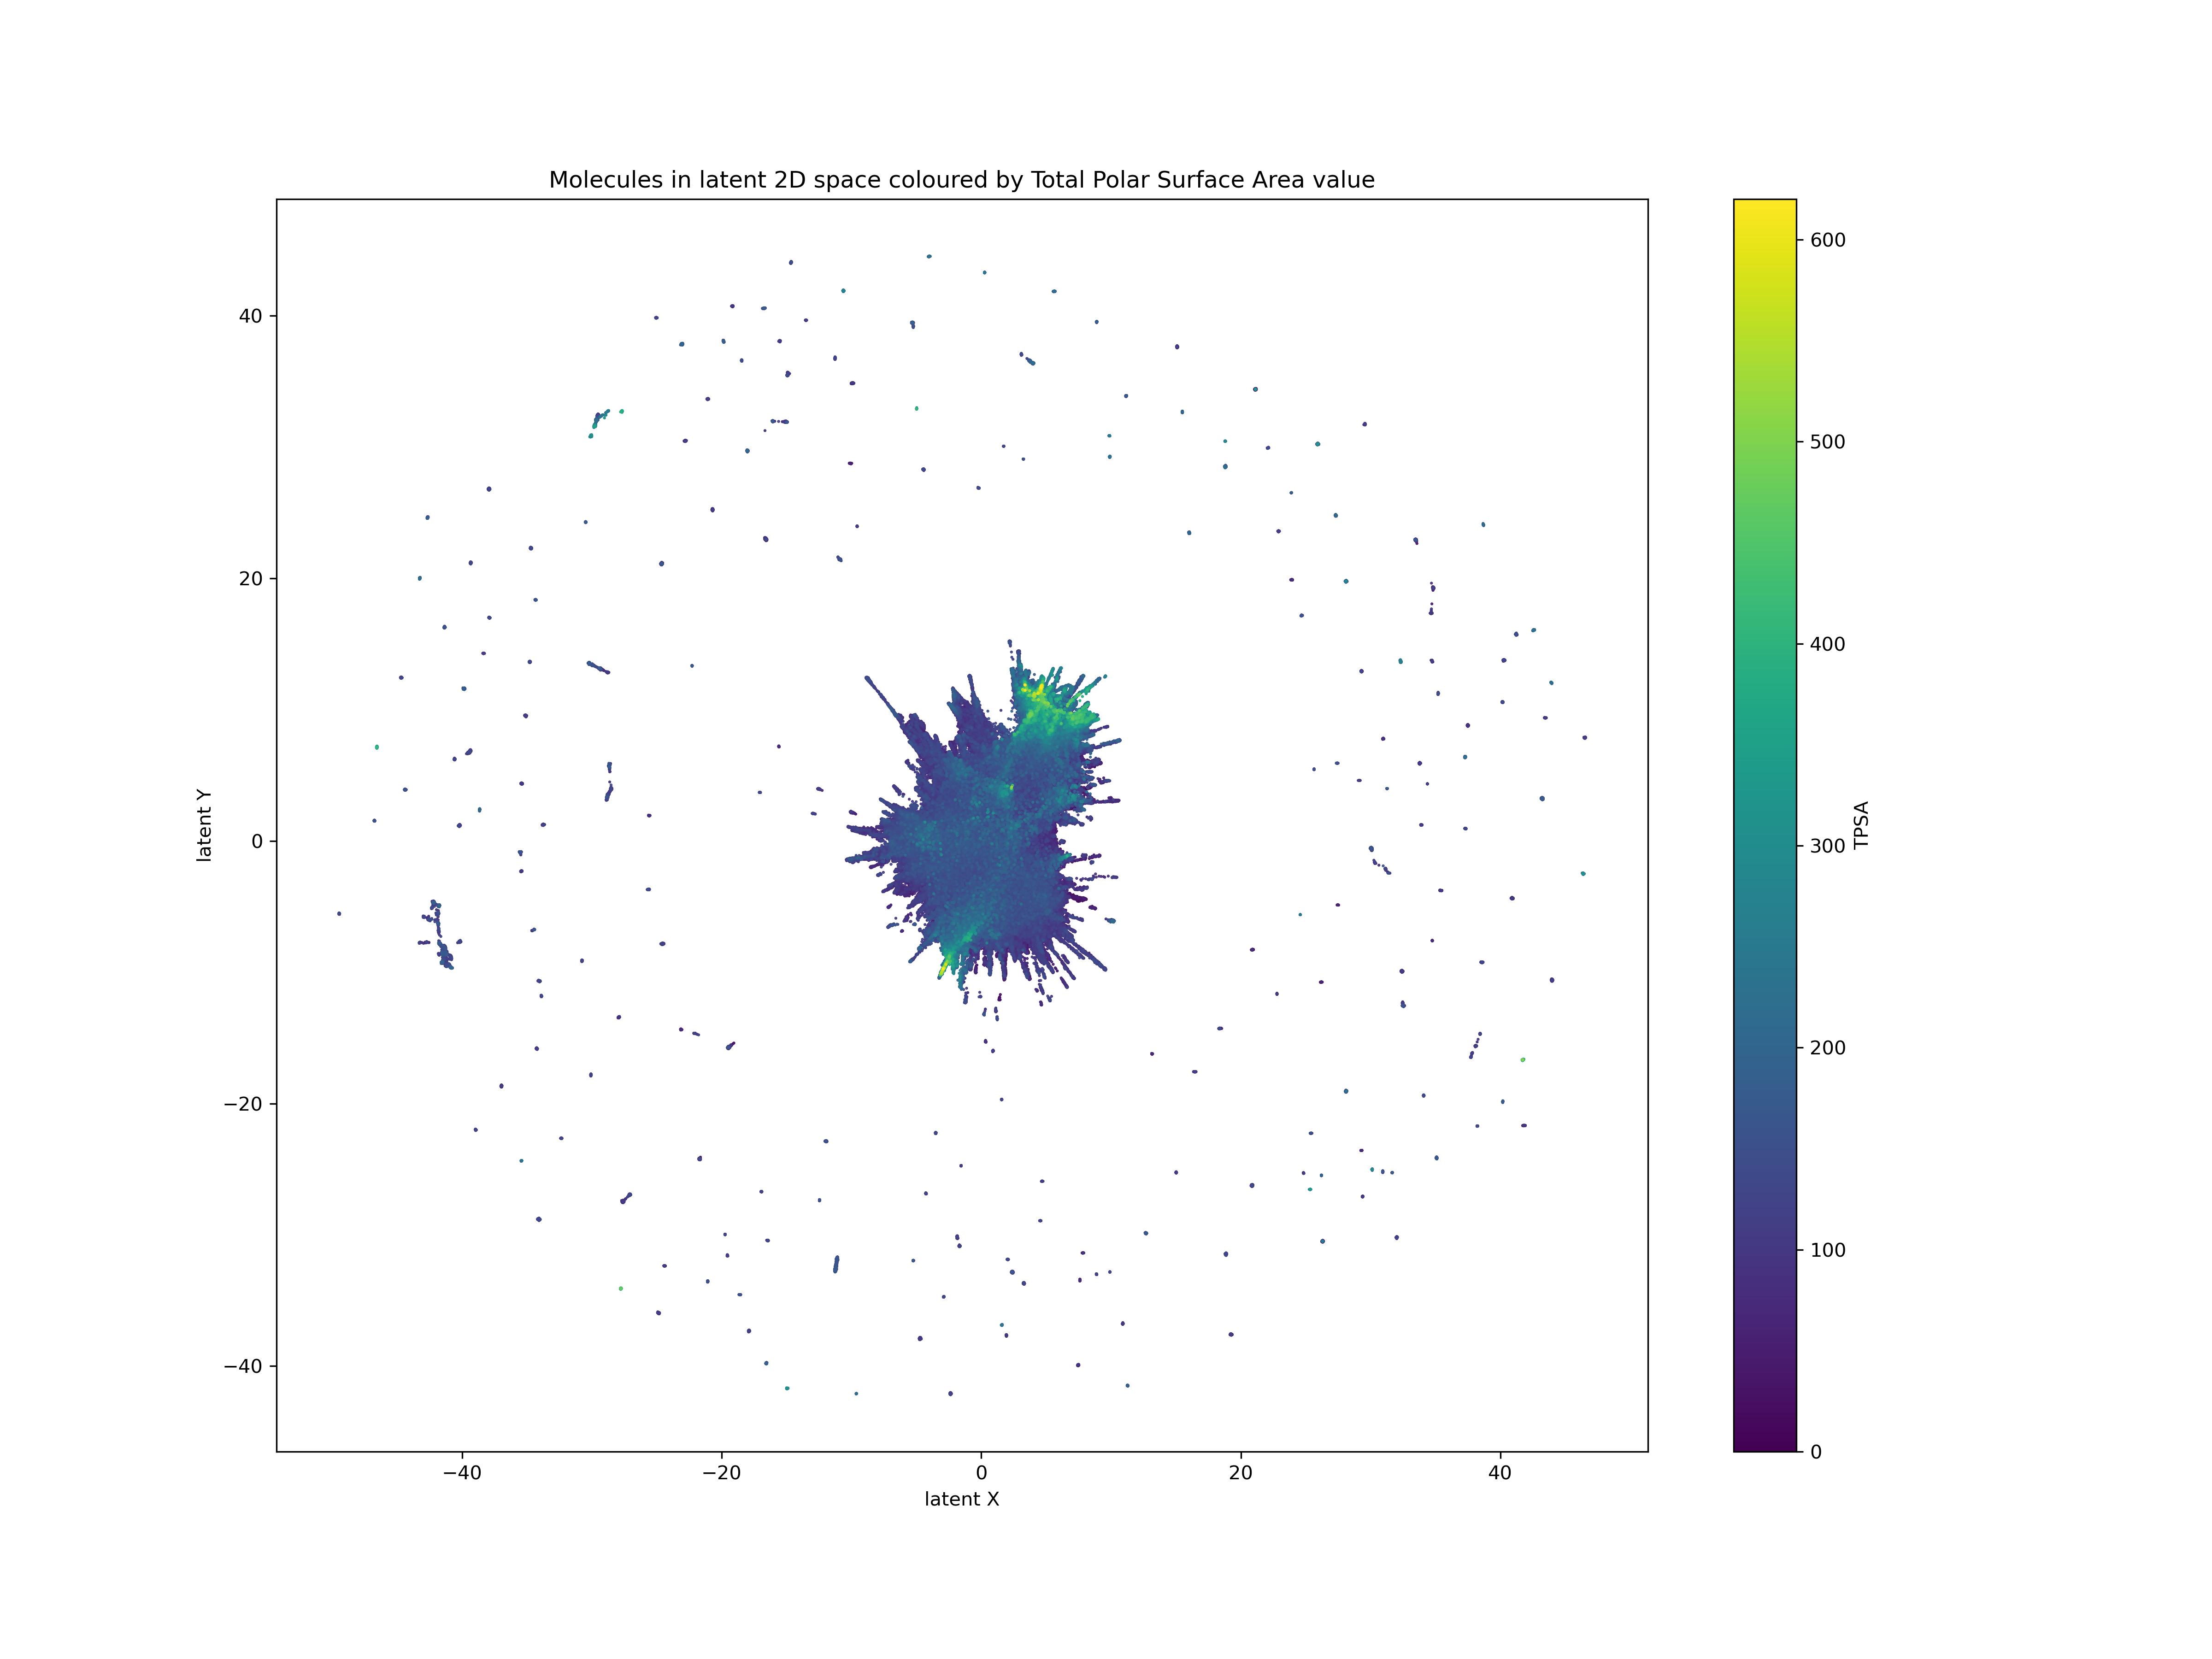
\includegraphics[width=0.49\columnwidth]{figures/TPSA_PaCMAP}
	\caption{Results of PCA, t-SNE, UMAP, TriMAP and PaCMAP on the latent dataset, coloured by Topological Polar Surface Area (TPSA). This descriptor was not used by the property predictor in the making of the latent representation.}
	\label{fig:TPSA}
\end{figure}

The choice of descriptors matter because different metrics relate differently to chemical structure. For example, the melting point of a substance is affected mostly by the secondary bonds it can form. Consider \textit{ethane} and \textit{ethanol}. These two molecules are structurally very similar, only differing by one oxygen atom. This however changes the strongest secondary bond that can form between individual molecules. While solid ethane is bound together only by \textit{van der Waals forces}~\cite{bib:vanderwaals}, solid ethanol is held together by \textit{hydrogen bonds}~\cite{bib:hbond}, many times stronger. As such, while the melting point of ethane is $-182.8~^\circ$C, ethanol melts at $-114.14~^\circ$C. The difference is even more dramatic for boiling points, $-88.5~^\circ$C and $+78.23~^\circ$C for ethane and ethanol respectively.

The ideal descriptors are those that do not change very much as the structure of molecules changes a little. In the end, I chose the following metrics: Quantitative estimate of drug-likeness, Ring count, number of hydrogen donors, number of hydrogen acceptors, topological polar surface area~\cite{bib:tpsa} and number of rotatable bonds.

It should be noted that some of these descriptors do jump slightly from molecule to molecule, however, this change is not too great to cause problems in interpreting data.

As can be seen on figure (\ref{fig:default_run}), the different algorithms yielded in substantially different embeddings. This is a direct result of the differences highlighted in table (\ref{tab:graph}). 

PCA produces the smoothest transition. This might seem positive, but in reality, this is not ideal. Chemical descriptors, qed in particular are not monotonous over chemical structure. This means that similar while similar molecules have similar qed values, dissimilar molecules might have the exact same qed. For this reason, a complete gradient is undesirable. This stems from the fact that PCA performs a linear transformation, not allowing for the preservation of such structures.

Another interesting thing is the difference in sklearn t-SNE and tsnecuda (second and third graph respectively). The sklearn implementation did not differentiate dissimilar points into distinct clusters. Investigating this phenomenon lead to the discovery that sklearn's implementation was bugged, only iterating for a mere 150 iteration, which was not enough for separation of different molecules, as can be seen on figure (\ref{fig:tsne:iter_sweep}). t-SNE has the most uniform clustering in terms of density of points among the graph-based algorithms. It should be noted that t-SNE did not use the default perplexity value, as I have found previously that a perplexity parameter of around 1000 produces the most desirable output. 

UMAP clusters the molecules in one big cluster (although not as extremely as PaCMAP), with a few little clusters on the side. This is partly due to the low default min\_dist parameter, making ultra-tightly packed clusters. The space is very much smooth over qed value. 

TriMAP creates objects resembling magnetic field lines. This is very interesting from a structural view. It should be noted however, that it seems like the individual clusters overlap with each other in a way that no other algorithm resembles. For this reason, targeted search would be very difficult on a space created by TriMAP. This particular problem as we will see does not get better with tuning parameters, making TriMAP fundamentally unusable for this use-case.

PaCMAP -- similarly to UMAP -- produces one compact cluster in the middle, with some additional clusters nearby. This behaviour is not ideal for targeted search, since quite different molecules are placed near each other. PaCMAP does offer very much control over its sightedness however, and with different parameters, this can change.

In determining whether the space is smooth over the chemical structure of molecules instead of some descriptors, I investigated the embeddings by colouring the plots according to descriptors that have definitely not been used by the property predictor during the training of the VAE. As can be seen on figure (\ref{fig:TPSA}), colouring by topological polar surface area, It can be stated that the algorithms produce a smooth gradient between high-valued areas and lower-valued areas. This indicates that the space is indeed smooth over the chemical structure. Multiple other descriptors have been tested and they all yielded similar results.

Overall, with default parameters, it initially seems like t-SNE produces the most desirable embedding. TriMAP resulted in the least useful output space out of the graph-based algorithms. This will however change with other parameters, as the values are tuned to represent the dataset faithfully.

\section{Optimizing the parameters}\label{sec:optimizing-the-parameters}

As discussed previously, an advantage of parametrizable algorithms is the fact that the user is able to influence the preservation of local or global structure according to their use-case. For optimal results, each algorithm was run multiple times with different parametrization. The choice of parameters to sweep was based on how much effect it had theoretically. 

\subsection{t-SNE}

There are many common parameters of graph-based algorithms, mainly because of the use of gradient descent. Indeed, the effect of these parameters do not have significantly different effects with other methods. Because of this, I will only present the parameters associated with GD with t-SNE.

The optimization of gradient descent is in and of itself a vast topic worth many books. In fact, many papers have been written on this very topic. The graph-based algorithms all use gradient descent and all have some form of optimization laid out in their respective original papers. For this reason, the only parameter I will show now is the number of iterations. This is one of the most important parameters of gradient descent as too few iterations will inevitably prevent the convergence on a local minimum, while too many iterations needlessly increases the runtime of the algorithm and can even lead to overfitting, the production of an analysis that corresponds too closely or exactly to a particular set of data, and may therefore fail to fit additional data or predict future observations reliably.

\begin{figure}[!h]
	\centering
	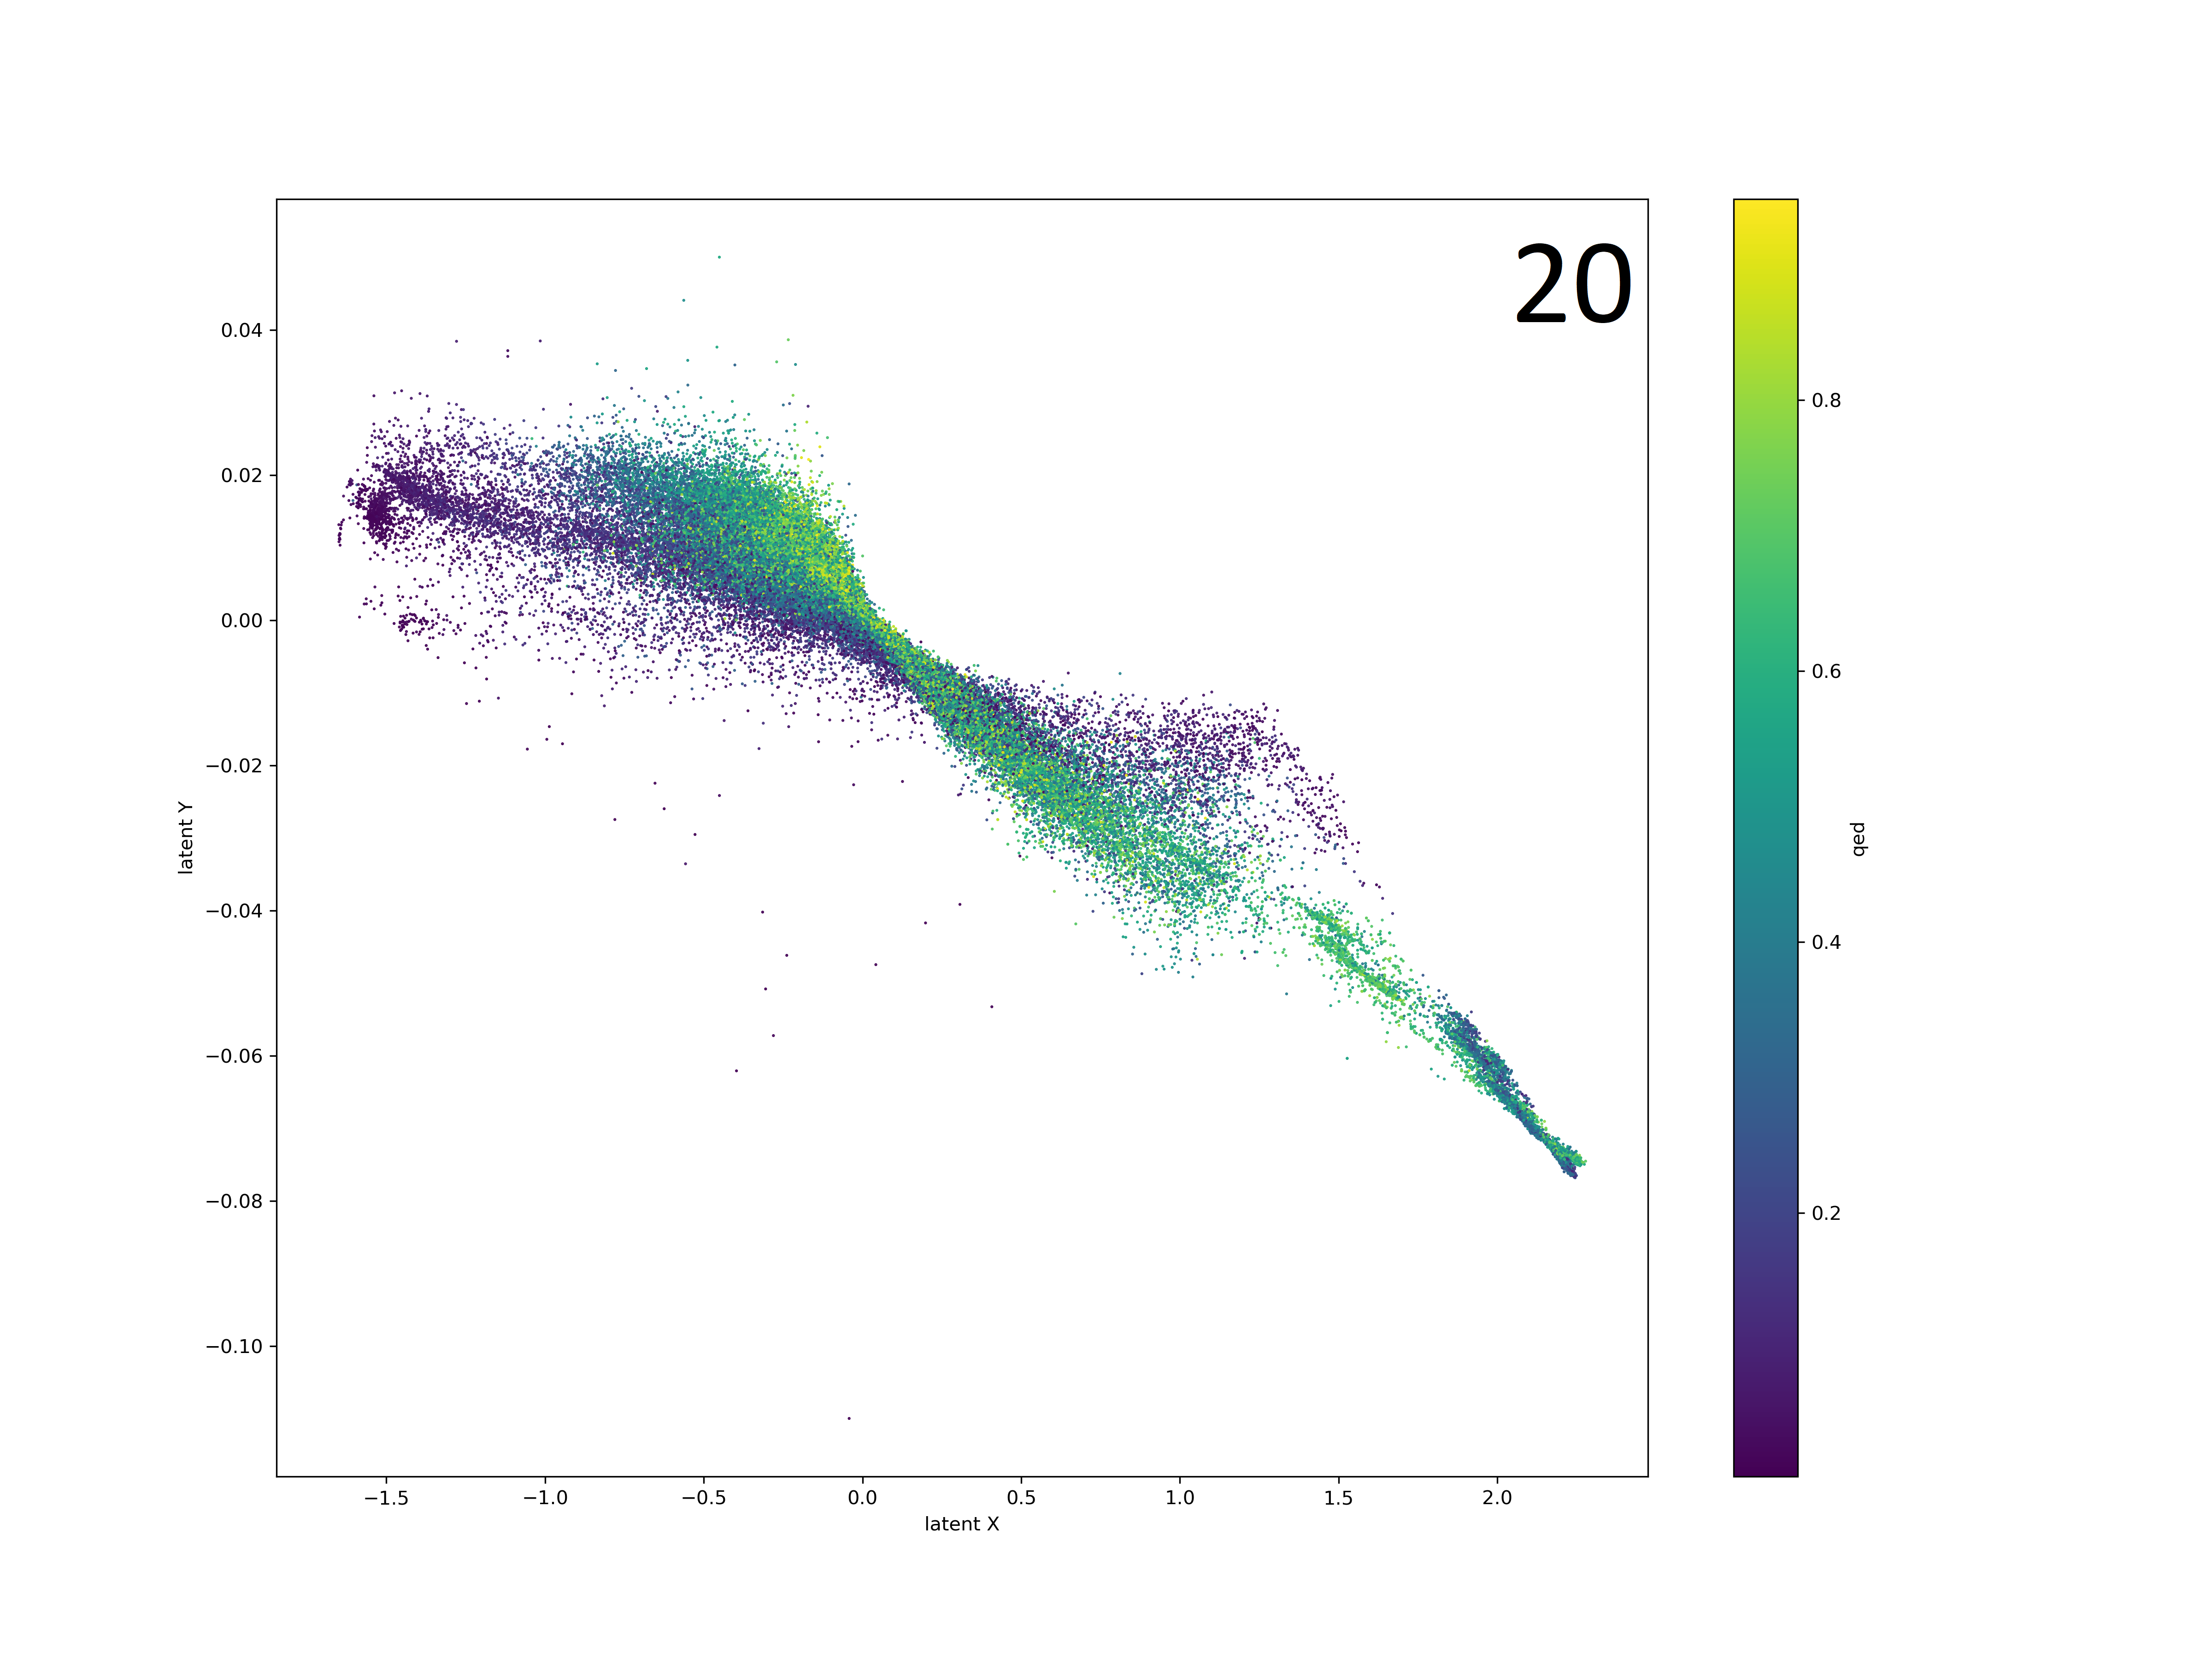
\includegraphics[width=0.45\columnwidth]{figures/qed20iter}
	\includegraphics[width=0.45\columnwidth]{figures/qed50iter}
	\includegraphics[width=0.45\columnwidth]{figures/qed200iter}
	\includegraphics[width=0.45\columnwidth]{figures/qed500iter}
	\includegraphics[width=0.45\columnwidth]{figures/qed1000iter}
	\caption{Result of the same t-SNE run after 20, 50, 200, 500 and 1000 iterations. The initial closeness of points comes from early exaggeration during gradient descent. It can be clearly seen that initial iterations change the embedding significantly, while later iterations only have minor effects.}
	\label{fig:tsne:iter_sweep}
\end{figure}

The effect of n\_iters does not scale linearly. In the initial iterations, the gradient of the error surface tends to be large, meaning that every step has a significant effect on the overall embedding. As the iterations go on however, the output approaches a local minimum, changing less and less every step. This effect is demonstrated by figure (\ref{fig:tsne:iter_sweep}), where in the first few hundred iterations significant change can be seen, while during the last 500 iterations only minor differences arise.

The most important parameter of t-SNE is perplexity. As described in section (\ref{sec:t-sne}), perplexity affects the $\sigma_i$ used in equation~\eqref{eq:tsne:pi|j}. This parameter is responsible for the focus between local and global structure preservation. This focus shift is rather limited in t-SNE, as figure (\ref{fig:tsne:perplexity}) shows.

\begin{figure}[!h]
	\centering
	\includegraphics[width=0.49\columnwidth]{figures/tsne_qed50perpl}
	\includegraphics[width=0.49\columnwidth]{figures/tsne_qed450perpl}
	\includegraphics[width=0.49\columnwidth]{figures/tsne_qed700perpl}
	\caption{Effect of perplexity on t-SNE. The values 50, 450 and 700 were used on a subset ($n = 100000$) of the whole database. Even significantly different perplexity values generate similar embeddings.}
	\label{fig:tsne:perplexity}
\end{figure}

It seems like this parameter does not have a large effect on the result. This can be attributed to the fact that perplexity does not directly affect the algorithm, only indirectly. Because of this, using the perplexity parameter does not allow fine control over the resulting embedding. It is possible that even higher, more extreme values of perplexity have more desirable effects, however, the memory consumption of $k$-nearest neighbour search for larger values of $k$ -- which is indirectly being increased with high perplexity -- renders it practically unusable.

\subsection{UMAP}


UMAP has two particularly interesting parameters when it comes to the result of the embedding. These are min\_dist and n\_neighbours. The former dictates the minimum distance between points that are in the same cluster, while the latter is the number of nearest neighbours searched for in the initial stage of the algorithm. 

The first parameter, min\_dist has a very drastic effect on the embedding. With low values of min\_dist, clusters there is no penality for placing intra-cluster points very closely, forming  highly compact clusters. This also means that different clusters are separated more clearly. With higher values, even points in the same cluster are placed further apart, making a more uniform distribution of points, that have less cluster separation. This effect is shown on figure (\ref{fig:umap:min_dist}). 

\begin{figure}[!h]
	\centering
	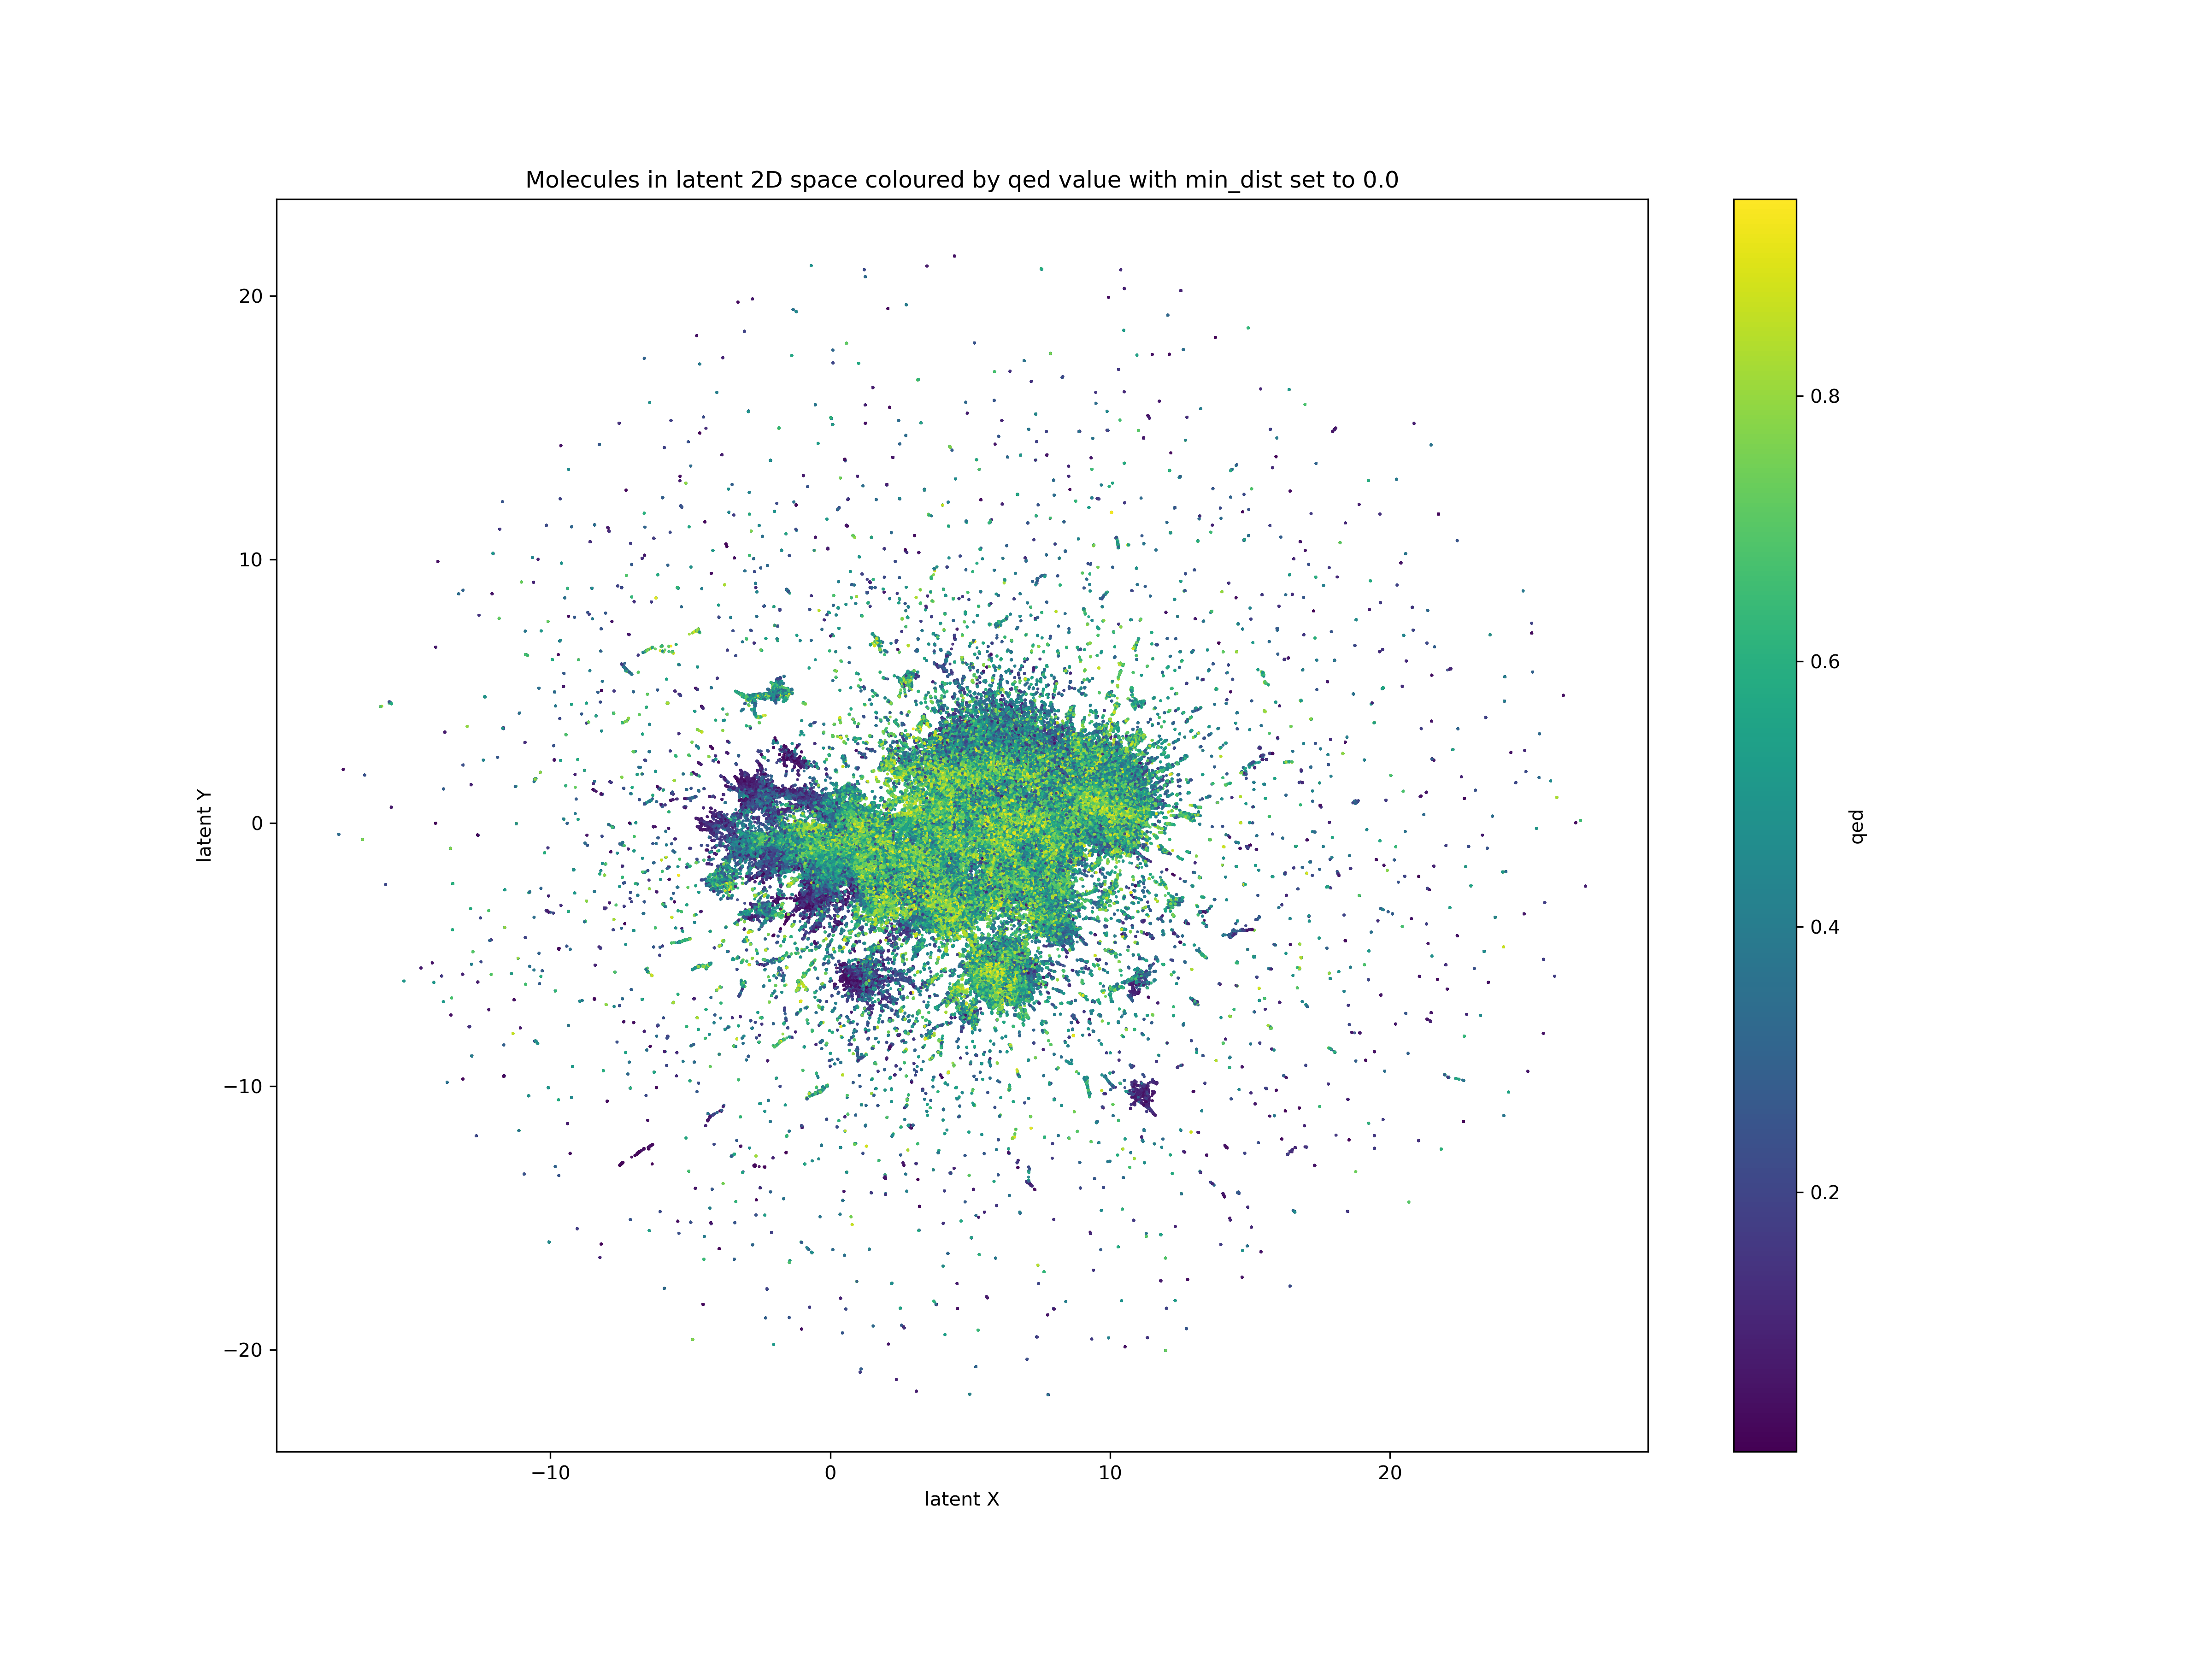
\includegraphics[width=0.49\columnwidth]{figures/UMAP0.0}
	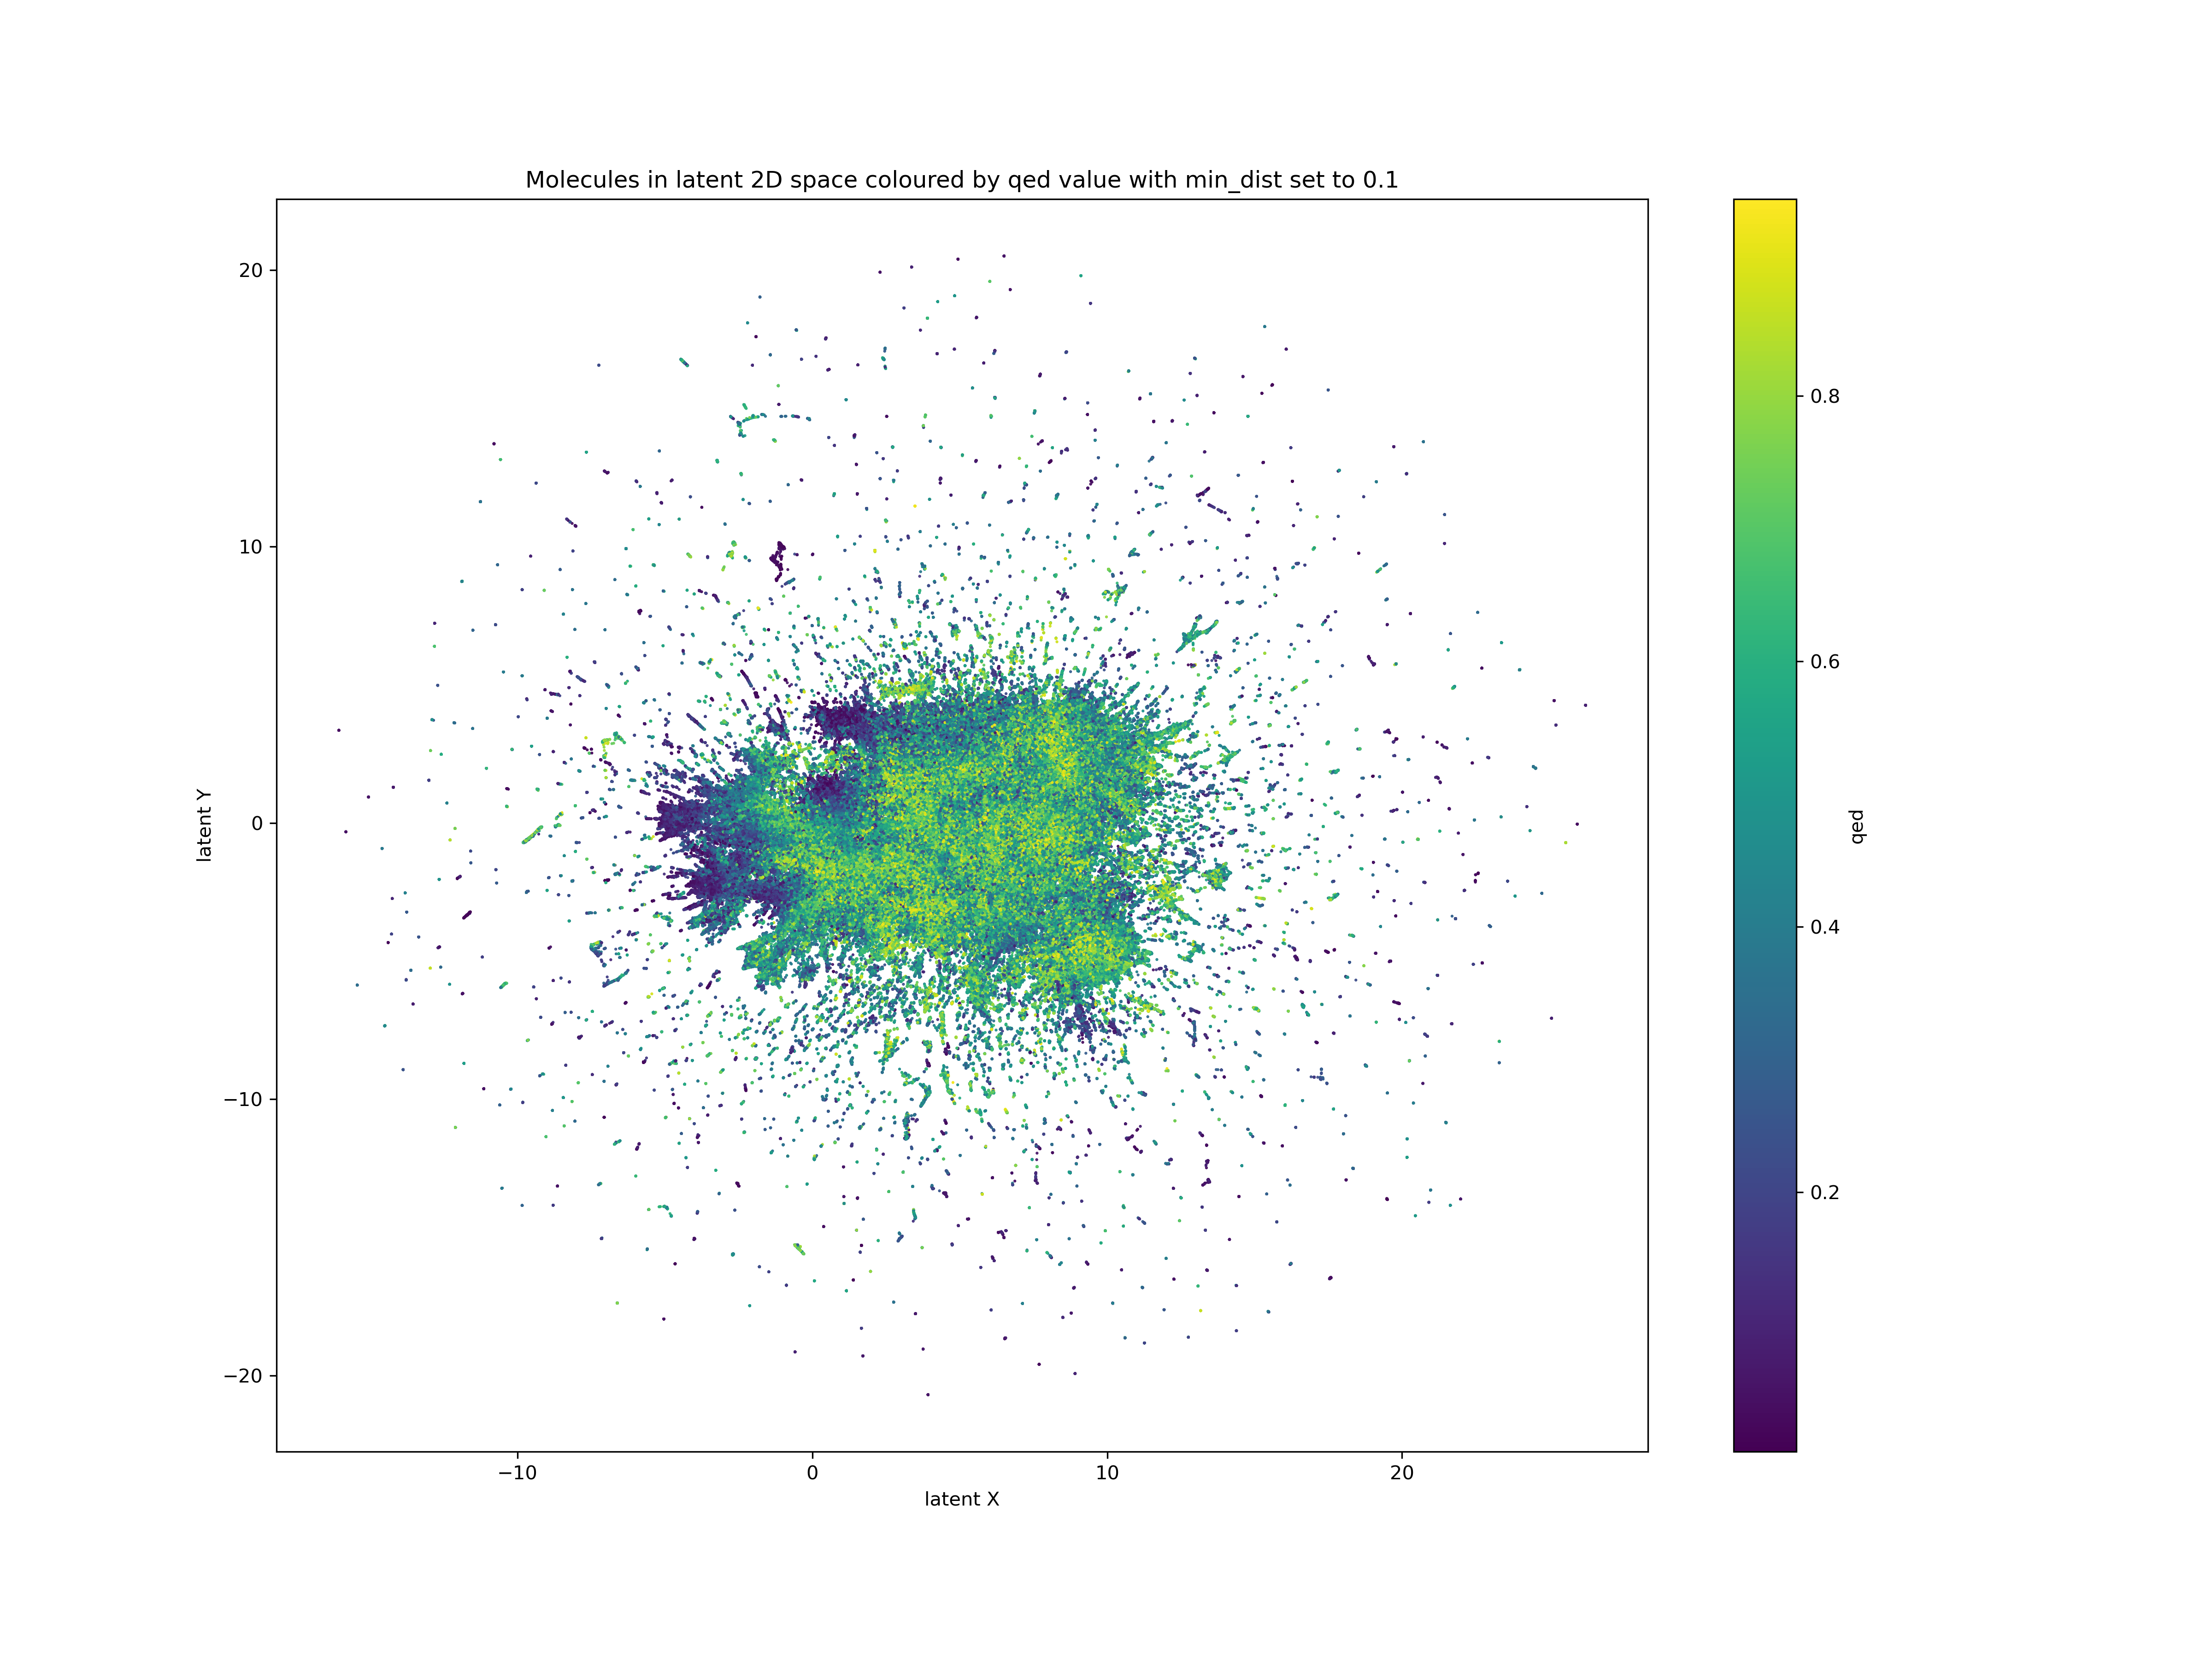
\includegraphics[width=0.49\columnwidth]{figures/UMAP0.1}
	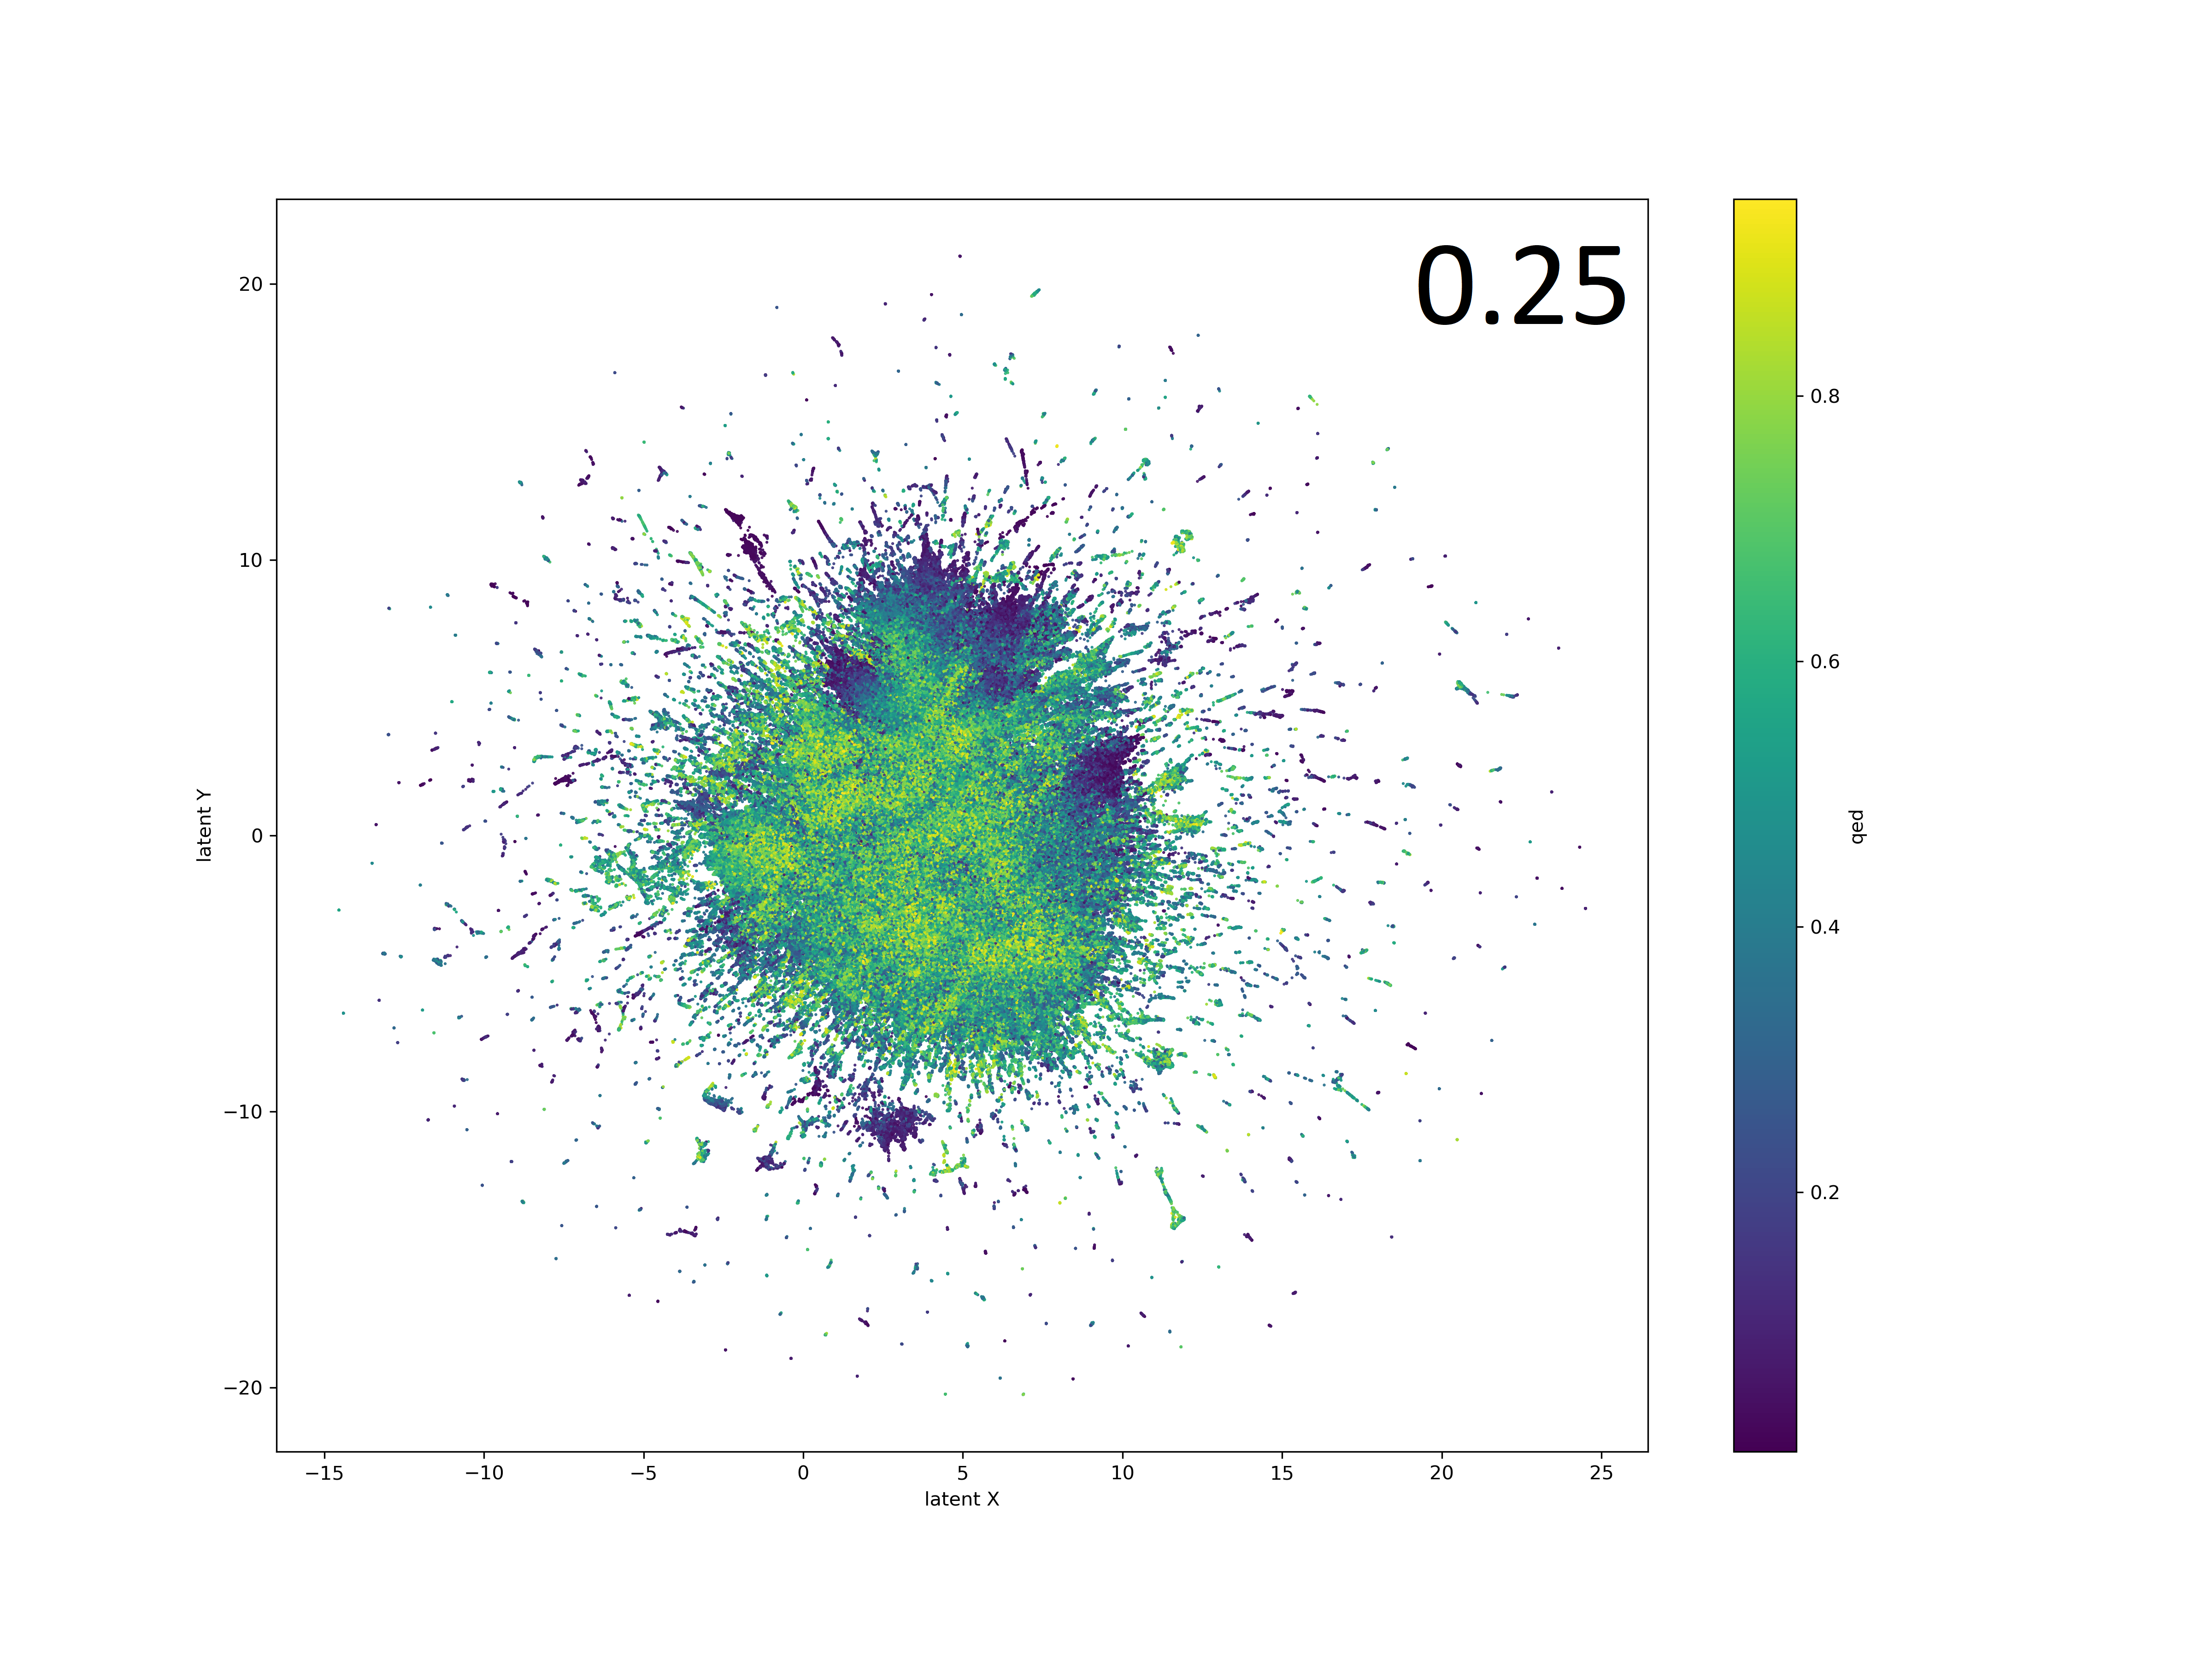
\includegraphics[width=0.49\columnwidth]{figures/UMAP0.25}
	\includegraphics[width=0.49\columnwidth]{figures/UMAP0.5}
	\includegraphics[width=0.49\columnwidth]{figures/UMAP0.75}
	\includegraphics[width=0.49\columnwidth]{figures/UMAP0.99}
	\caption{Effect of min\_dist parameter on the embedding produced by UMAP. The values are in order: 0.0, 0.1, 0.25, 0.5, 0.75 and 0.99. As the value increases, so does the space between points in the same cluster, making the whole space more spread out.}
	\label{fig:umap:min_dist}
\end{figure}

While the ultra-tight clusters allow more separation of inter-cluster molecules, for the purpose of targeted search, they are undesirable. This is due to the fact that in tightly-packed clusters, sampling must be done very closely to the original point, meaning even small changes in the location of a sampled point can result in very different chemicals. This however can be solved by generating the low min\_dist embedding and scaling every point too. The major drawback of such a procedure is that targeted searching in the scaled space results in scaled points that have to be rescaled for further use. 

While the exact optimum of this parameter is not objectively measurable, according to figure (\ref{fig:umap:min_dist}) a value of around 0.75 seems to be the sweet spot for balance between tightly packed clusters and uniformly placing the molecules. 

The number of nearest neighbours is the parameter of UMAP that shifts the focus from local to global structure. With a larger number of nearest neighbours, a more global structure is approximated in the initial stage of UMAP. This in turn results in the lower dimensional graph being optimized for more global structure preservation. 

\begin{figure}[!h]
	\centering
	\includegraphics[width=0.45\columnwidth]{figures/UMAP@0.75@10}
	\includegraphics[width=0.45\columnwidth]{figures/UMAP@0.75@30}
	\includegraphics[width=0.45\columnwidth]{figures/UMAP@0.75@50}
	\includegraphics[width=0.45\columnwidth]{figures/UMAP@0.75@100}
	\includegraphics[width=0.45\columnwidth]{figures/UMAP@0.75@200}
	\caption{Effect of n\_neighbours parameter at values of 10, 20, 30, 50, 100 and 200 with a min\_dist parameter of 0.75. Higher values result in more compact overall embedding, as more and more points are counted as nearest neighbours. At particularly high values (such as 200), very few distinct clusters are formed and all molecules are placed on top of each other just like with TriMAP.}
	\label{fig:umap:n_neighbor}
\end{figure}

As can bee seen on figure (\ref{fig:umap:n_neighbor}), the value of n\_neighbours has a drastic effect when changed from a low value to a slightly higher one, however, at larger values the difference in embedding starts to diminish. One interesting thing that can be seen on is the gradual disappearance of clusters in favour of a uniform blob. For targeted searching, this is potentially bad, since so many molecules are packed into one space. For this reason, very high values are undesirable for this use-case.

\subsection{TriMAP}

We have seen in section (\ref{sec:result-of-first-runs}) that TriMAP produced very poor results for allowing targeted search. With this in mind and with the knowledge of locally-focused algorithms have performed much better, The obvious parameter choice is one (or more) that focuses on local structure. Out of the three main hyperparameters (\texttt{n\_inliers}, \texttt{n\_outliers}, \texttt{n\_random}), the most relevant seems to be \texttt{n\_inliers}.

\begin{figure}[!h]
	\centering
	\includegraphics[width=0.45\columnwidth]{figures/TriMAPqed@20}
	\includegraphics[width=0.45\columnwidth]{figures/TriMAPqed@30}
	\includegraphics[width=0.45\columnwidth]{figures/TriMAPqed@50}
	\includegraphics[width=0.45\columnwidth]{figures/TriMAPqed@100}
	\caption{Different values of \texttt{n\_inliers} (20, 30, 50 and 100) on a TriMAP embedding. This parameter did not substantially change the embedding.}
	\label{fig:trimap:n_inliers}
\end{figure}

After running TriMAP with a few values of \texttt{n\_inliers}, the results showed very little change in the topology of the embedding (seen in figure (\ref{fig:trimap:n_inliers})). The first thought I had seeing this result was that TriMAP is unable to focus on local structure of the dataset. This was supported by most articles and papers I have read on the subject. 

This meant that TriMAP is just unfit for the use-case of targeted searching in the latent space of drug-like molecules. 

Later on, I realized that the parameter \texttt{n\_inliers} serves a similar role as PaCMAP's near-pair count, influencing mostly global structure preservation. It can be seen on figure (\ref{fig:trimap:n_inliers}) that increasing the parameter significantly does not change the result as much, specifically because TriMAP already focuses on global structure.

Unfortunately, by the time I realized this, I did not have enough time to sweep through other parameters, particularly \texttt{n\_outliers}, which boost the repulsive forces exerted by dissimilar points. In the future, I want to see that parameter's effect on the result, to give TriMAP its chance.

\subsection{PaCMAP}

PaCMAP has four main hyperparameters that change the topology of the resulting embedding. These are the the number of near pairs ($n_{NB}$), the ratio between mid-near pairs and near pairs (MN\_ratio), the ratio between further pairs and near pairs (FP\_ratio) and the initialization of the lower dimensional graph. The original paper~\cite{bib:pacmap} describes the effect of changing each one briefly. 

The paper showed that PaCMAP is rather robust to the choice of initialization, more so than all other algorithms. For this reason, I decided not to investigate this parameter, as it would have lead to unfruitful optimizing.

The number of near pairs have a significant effect on the final embedding. In general, it can be said that for larger values of $n_{NB}$, PaCMAP preserves more global structure. This is due to the fact that increasing the nearest neighbours increases the attractive forces during optimization, resulting in a less overall detail in the embedding. 

MN\_ratio has very little effect on the overall embedding. Only by having extreme values of it (both extremely small and large), does it affect the result. It is observed that extreme values of MN\_ratio cause problems with both local and global structure. The omission of mid-near points cause the worst result, leading to no structural preservation. In the paper, it is stated that this ratio should be fixed to the default 0.5, for computational and quality reasons.

The effect of FP\_ratio on the resulting embedding is the exact opposite of that of $n_{NB}$. By sampling more further points, the repelling forces increase during optimization, leading to a more locally faithful representation of the original data.

\begin{figure}[!h]
	\centering
	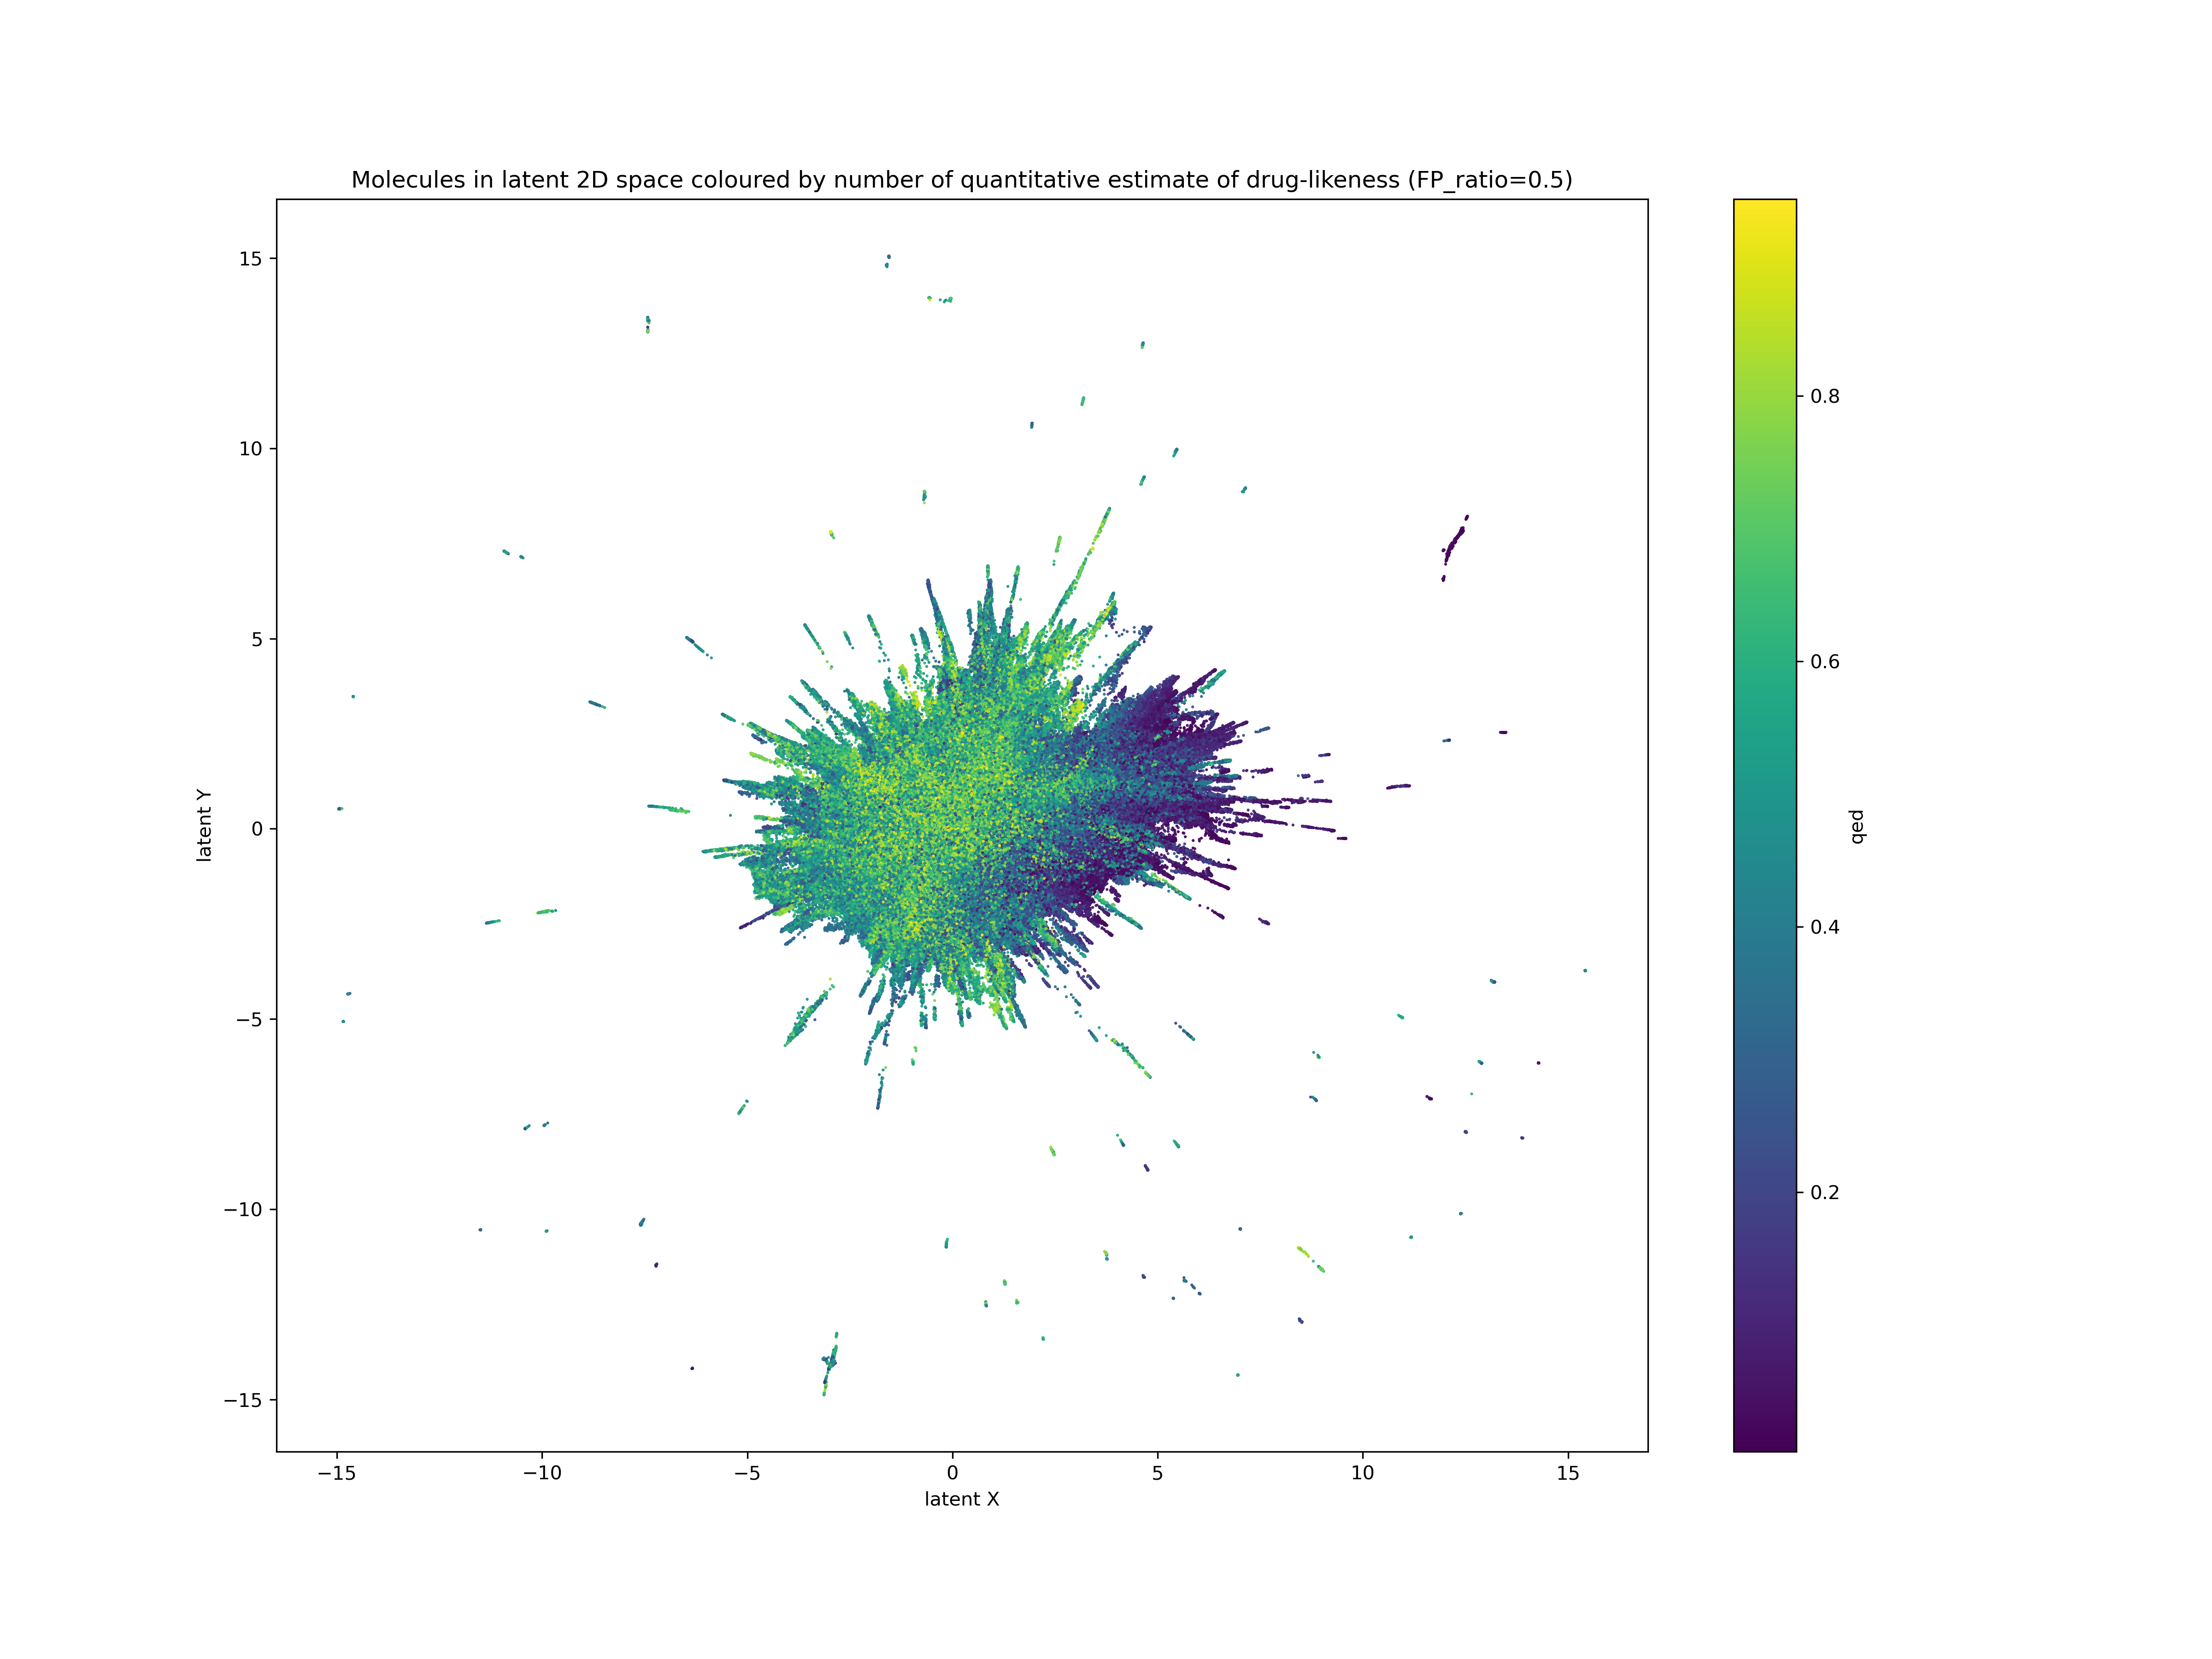
\includegraphics[width=0.45\columnwidth]{figures/PaCMAPqed@0.5}
	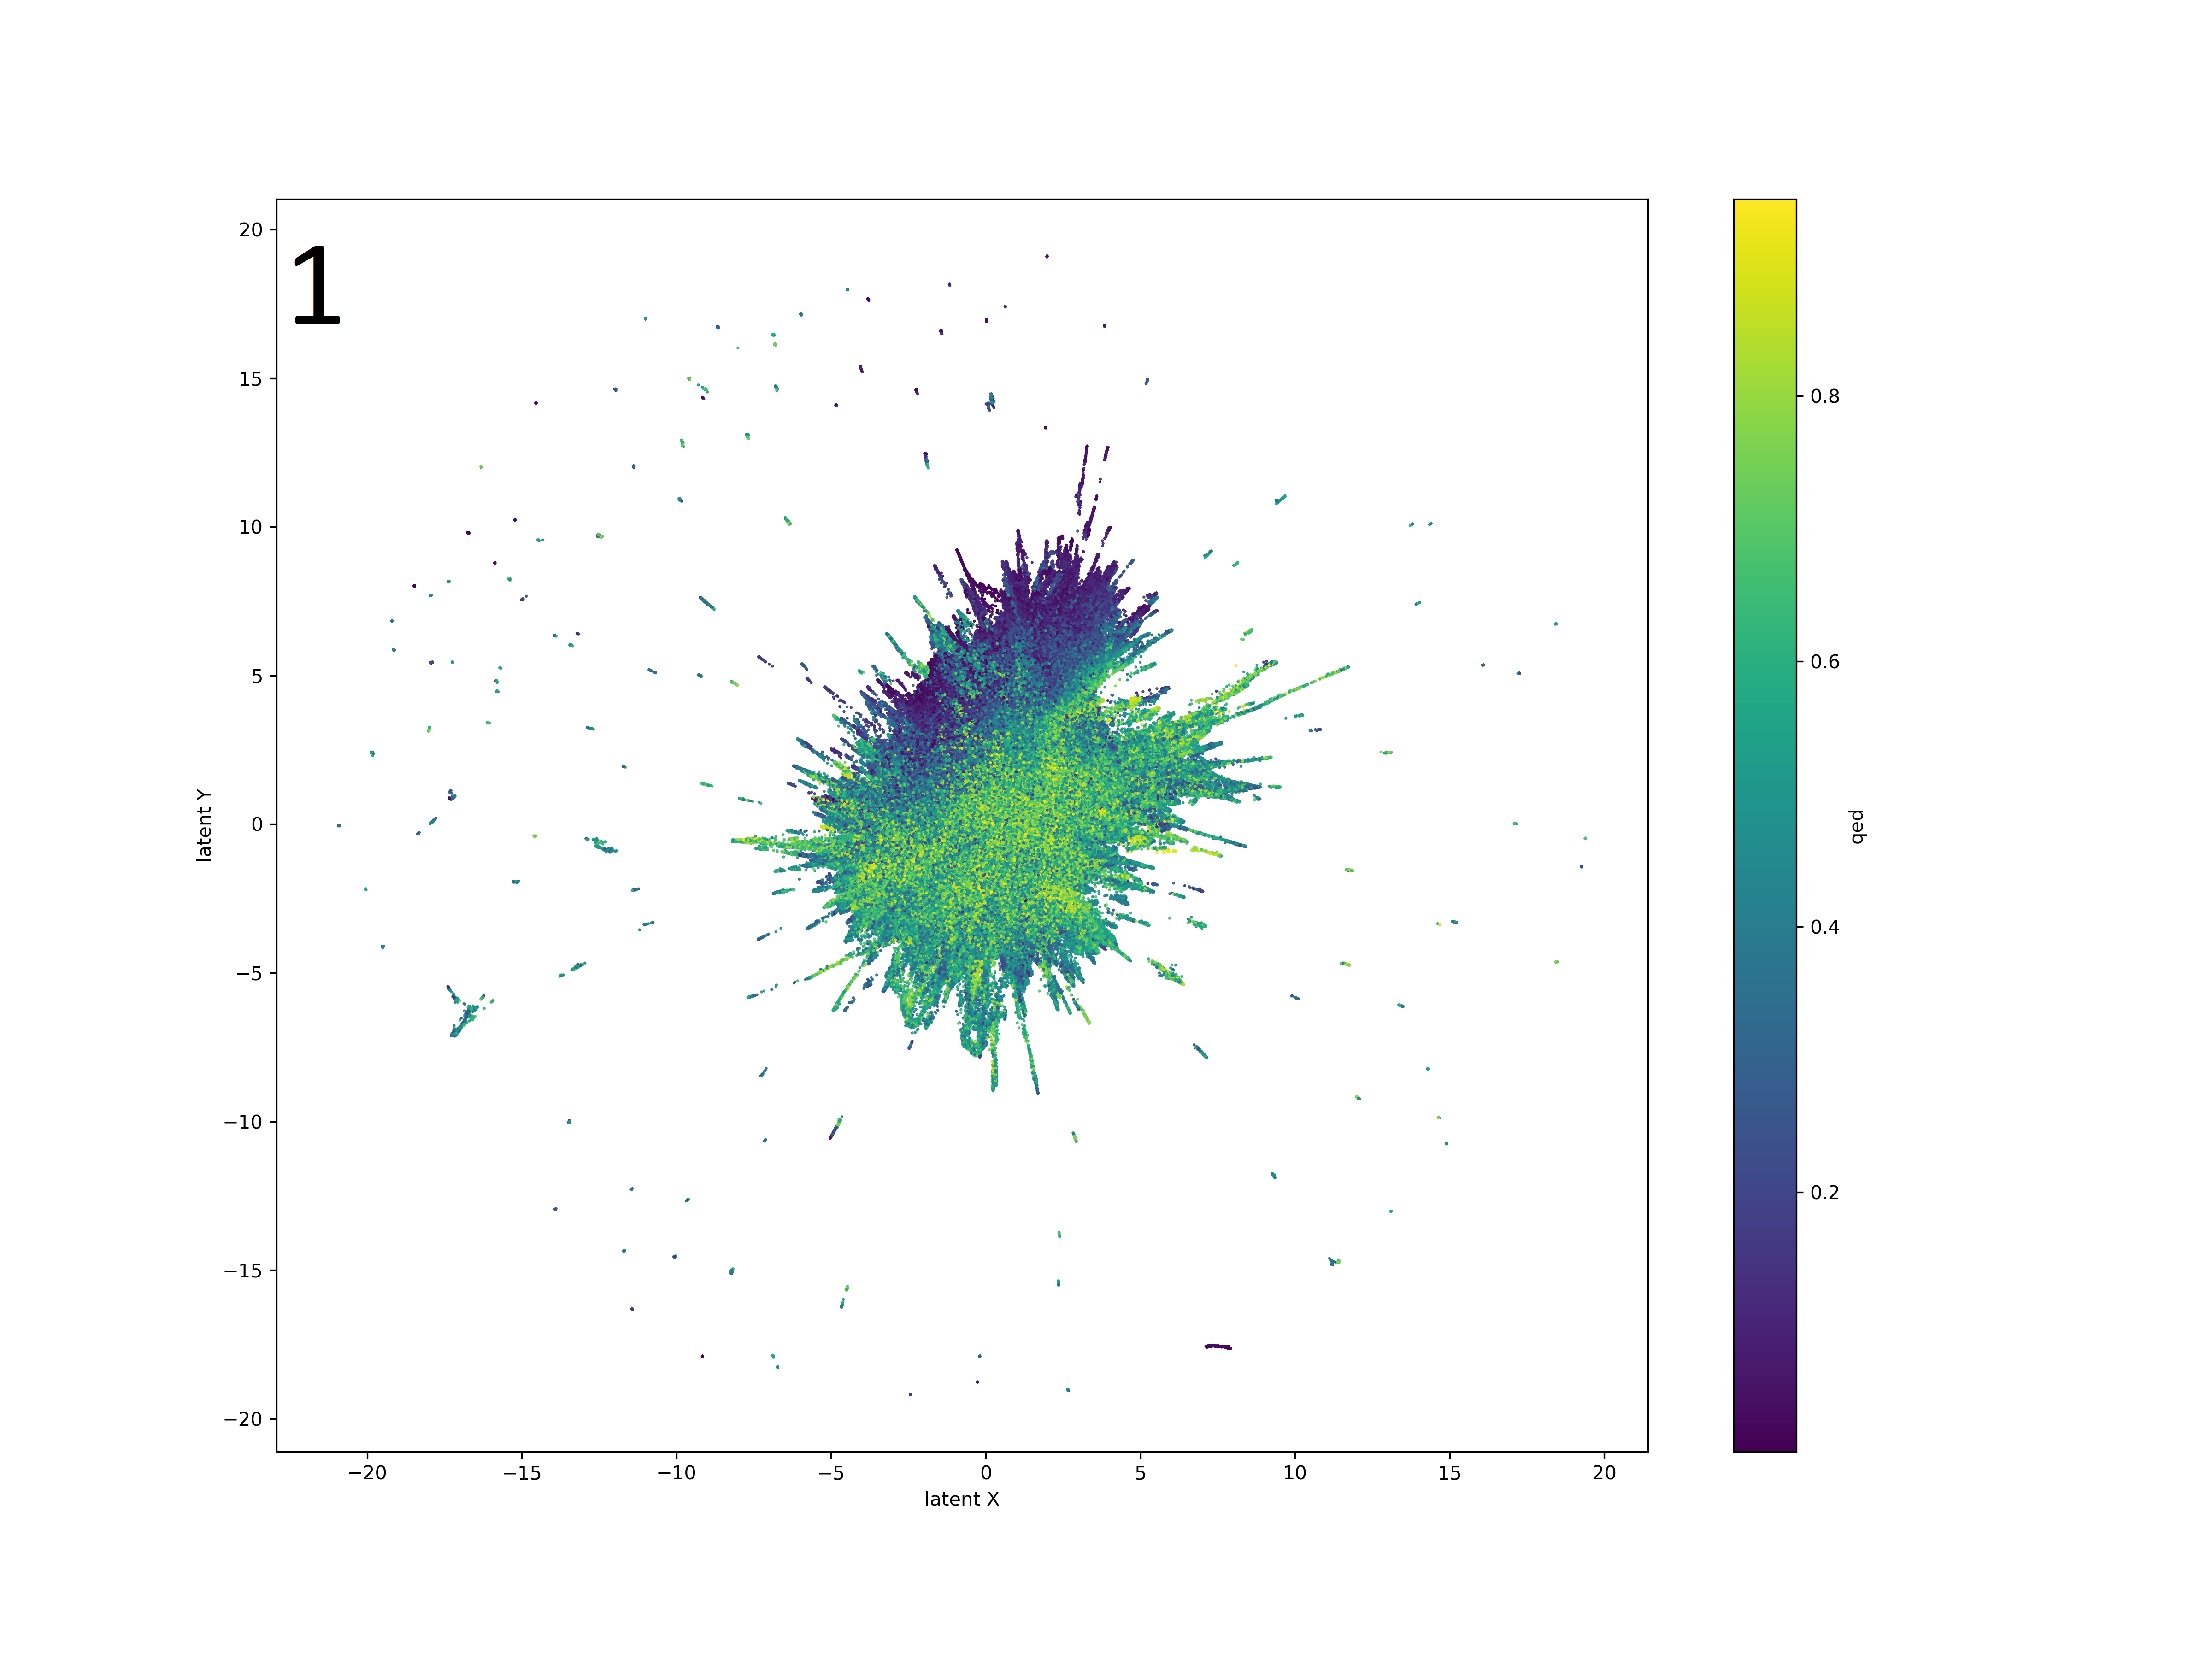
\includegraphics[width=0.45\columnwidth]{figures/PaCMAPqed@1}
	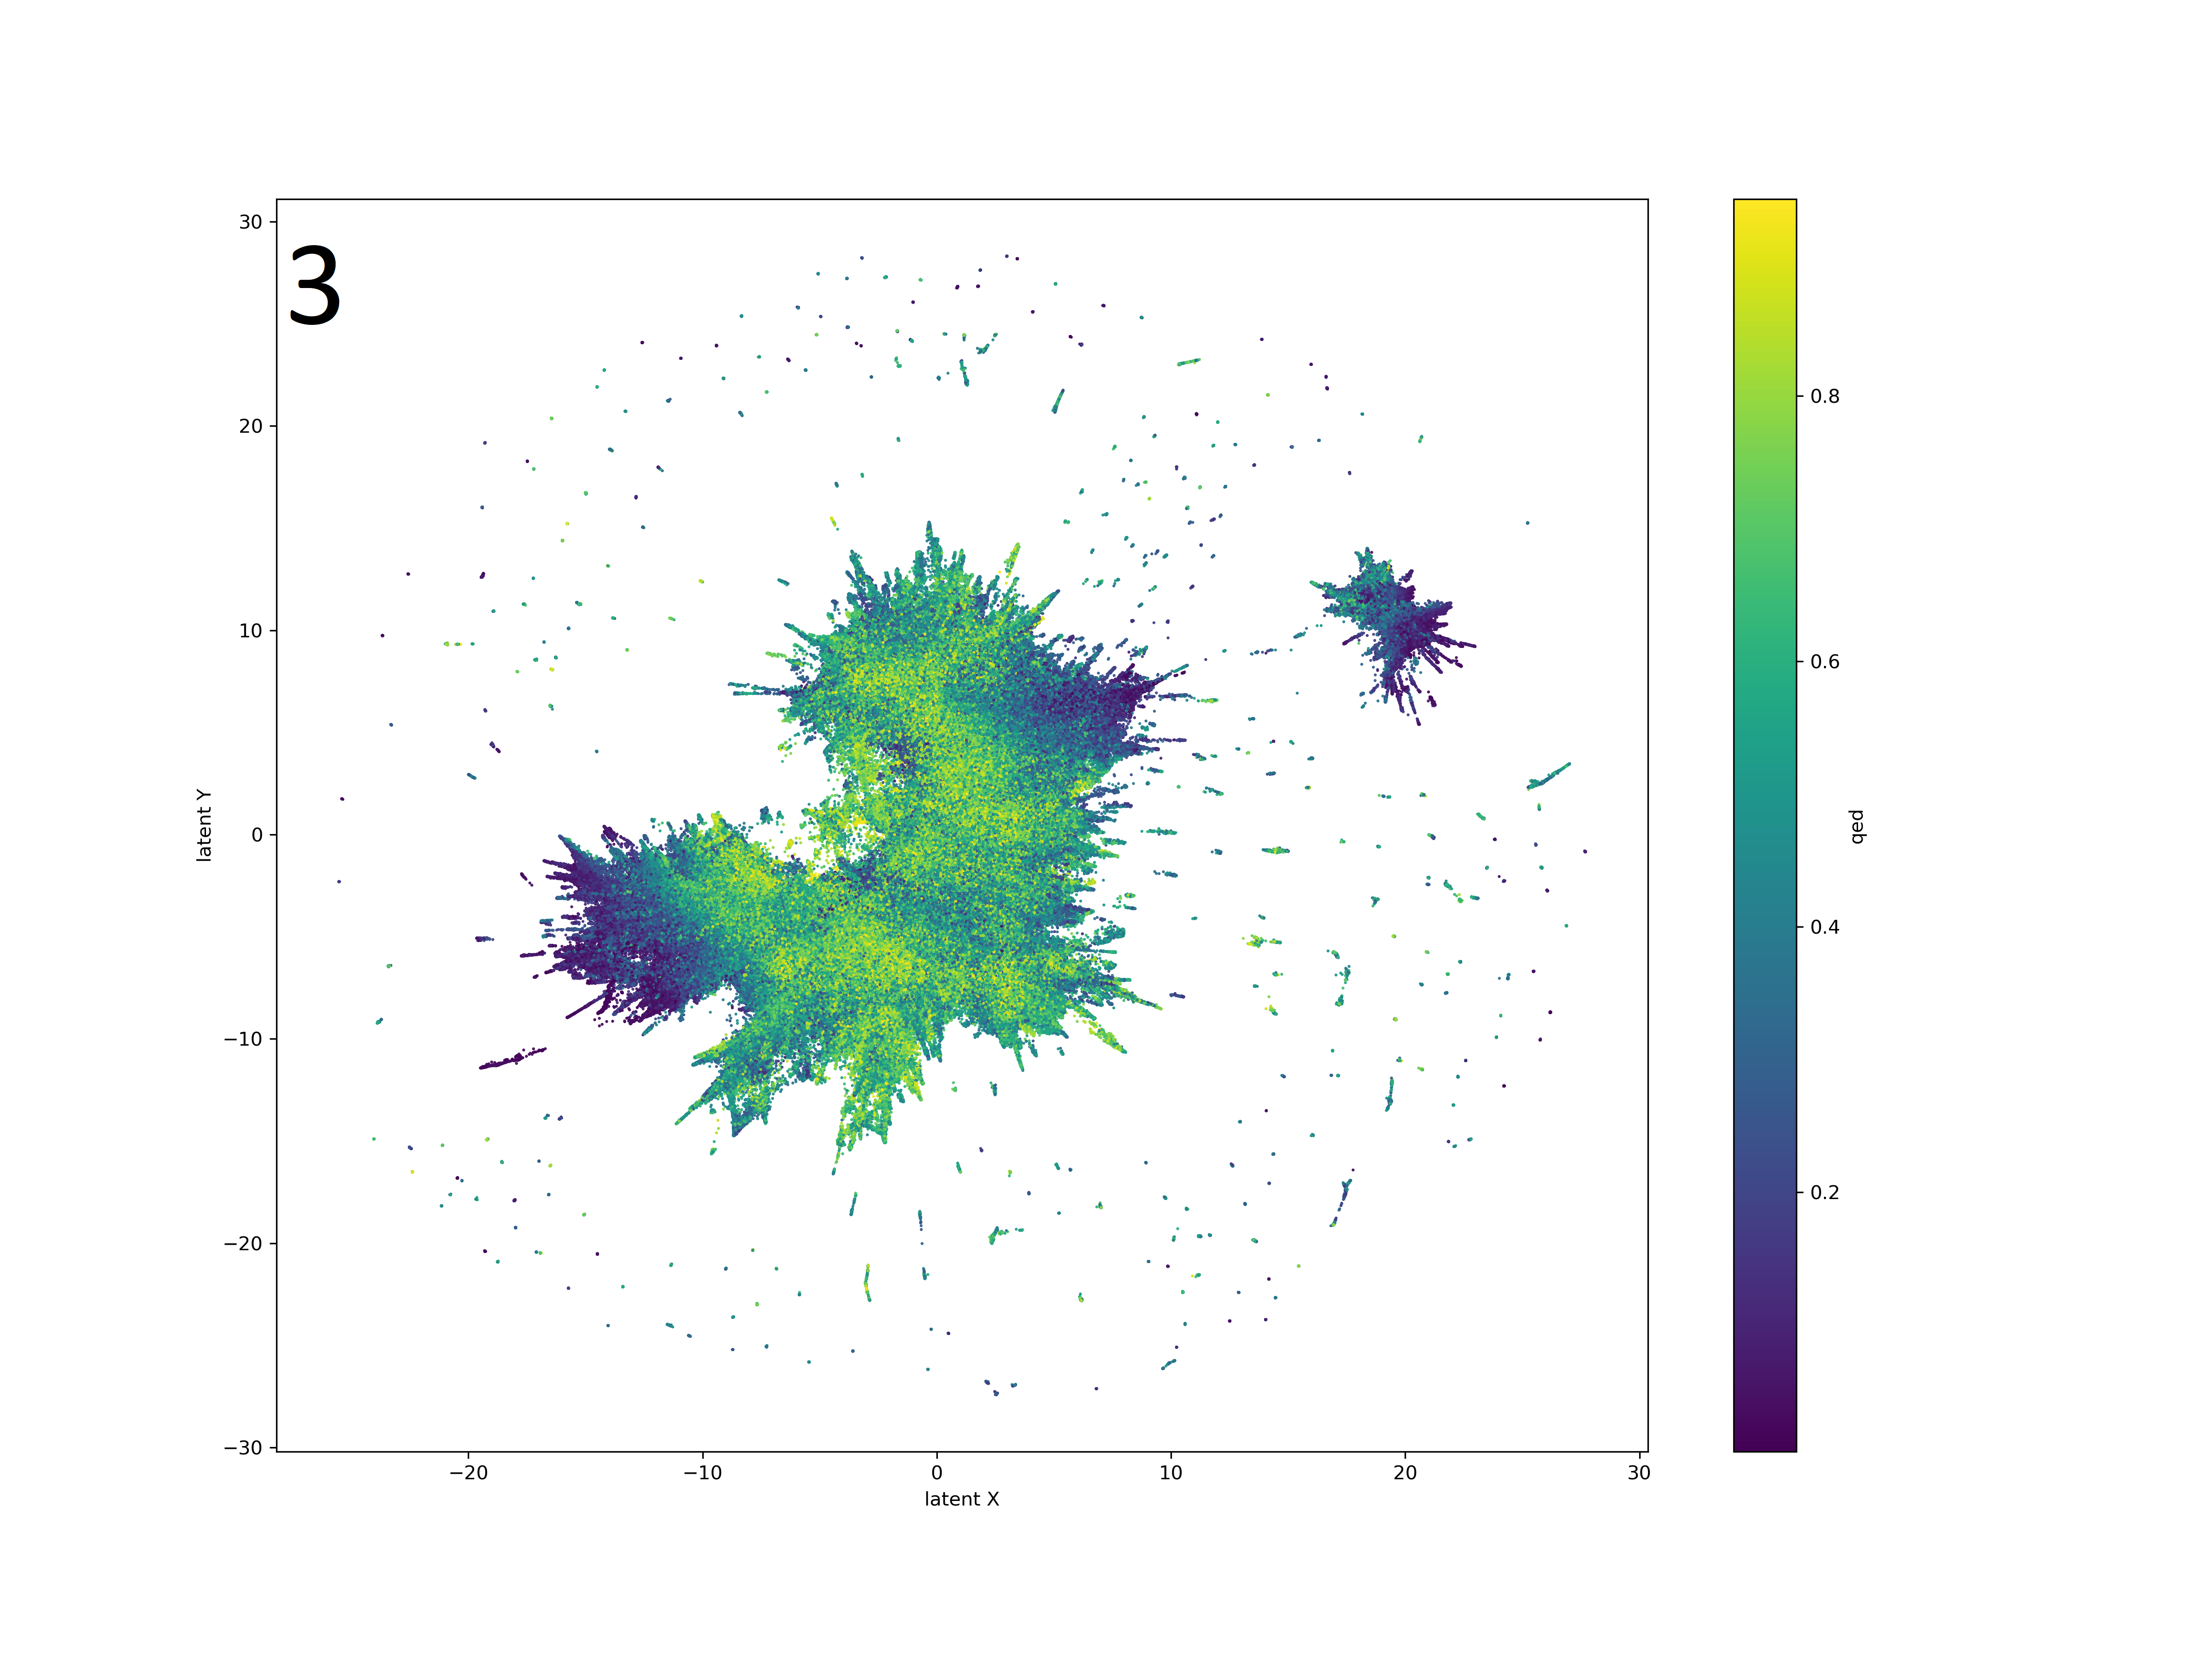
\includegraphics[width=0.45\columnwidth]{figures/PaCMAPqed@3}
	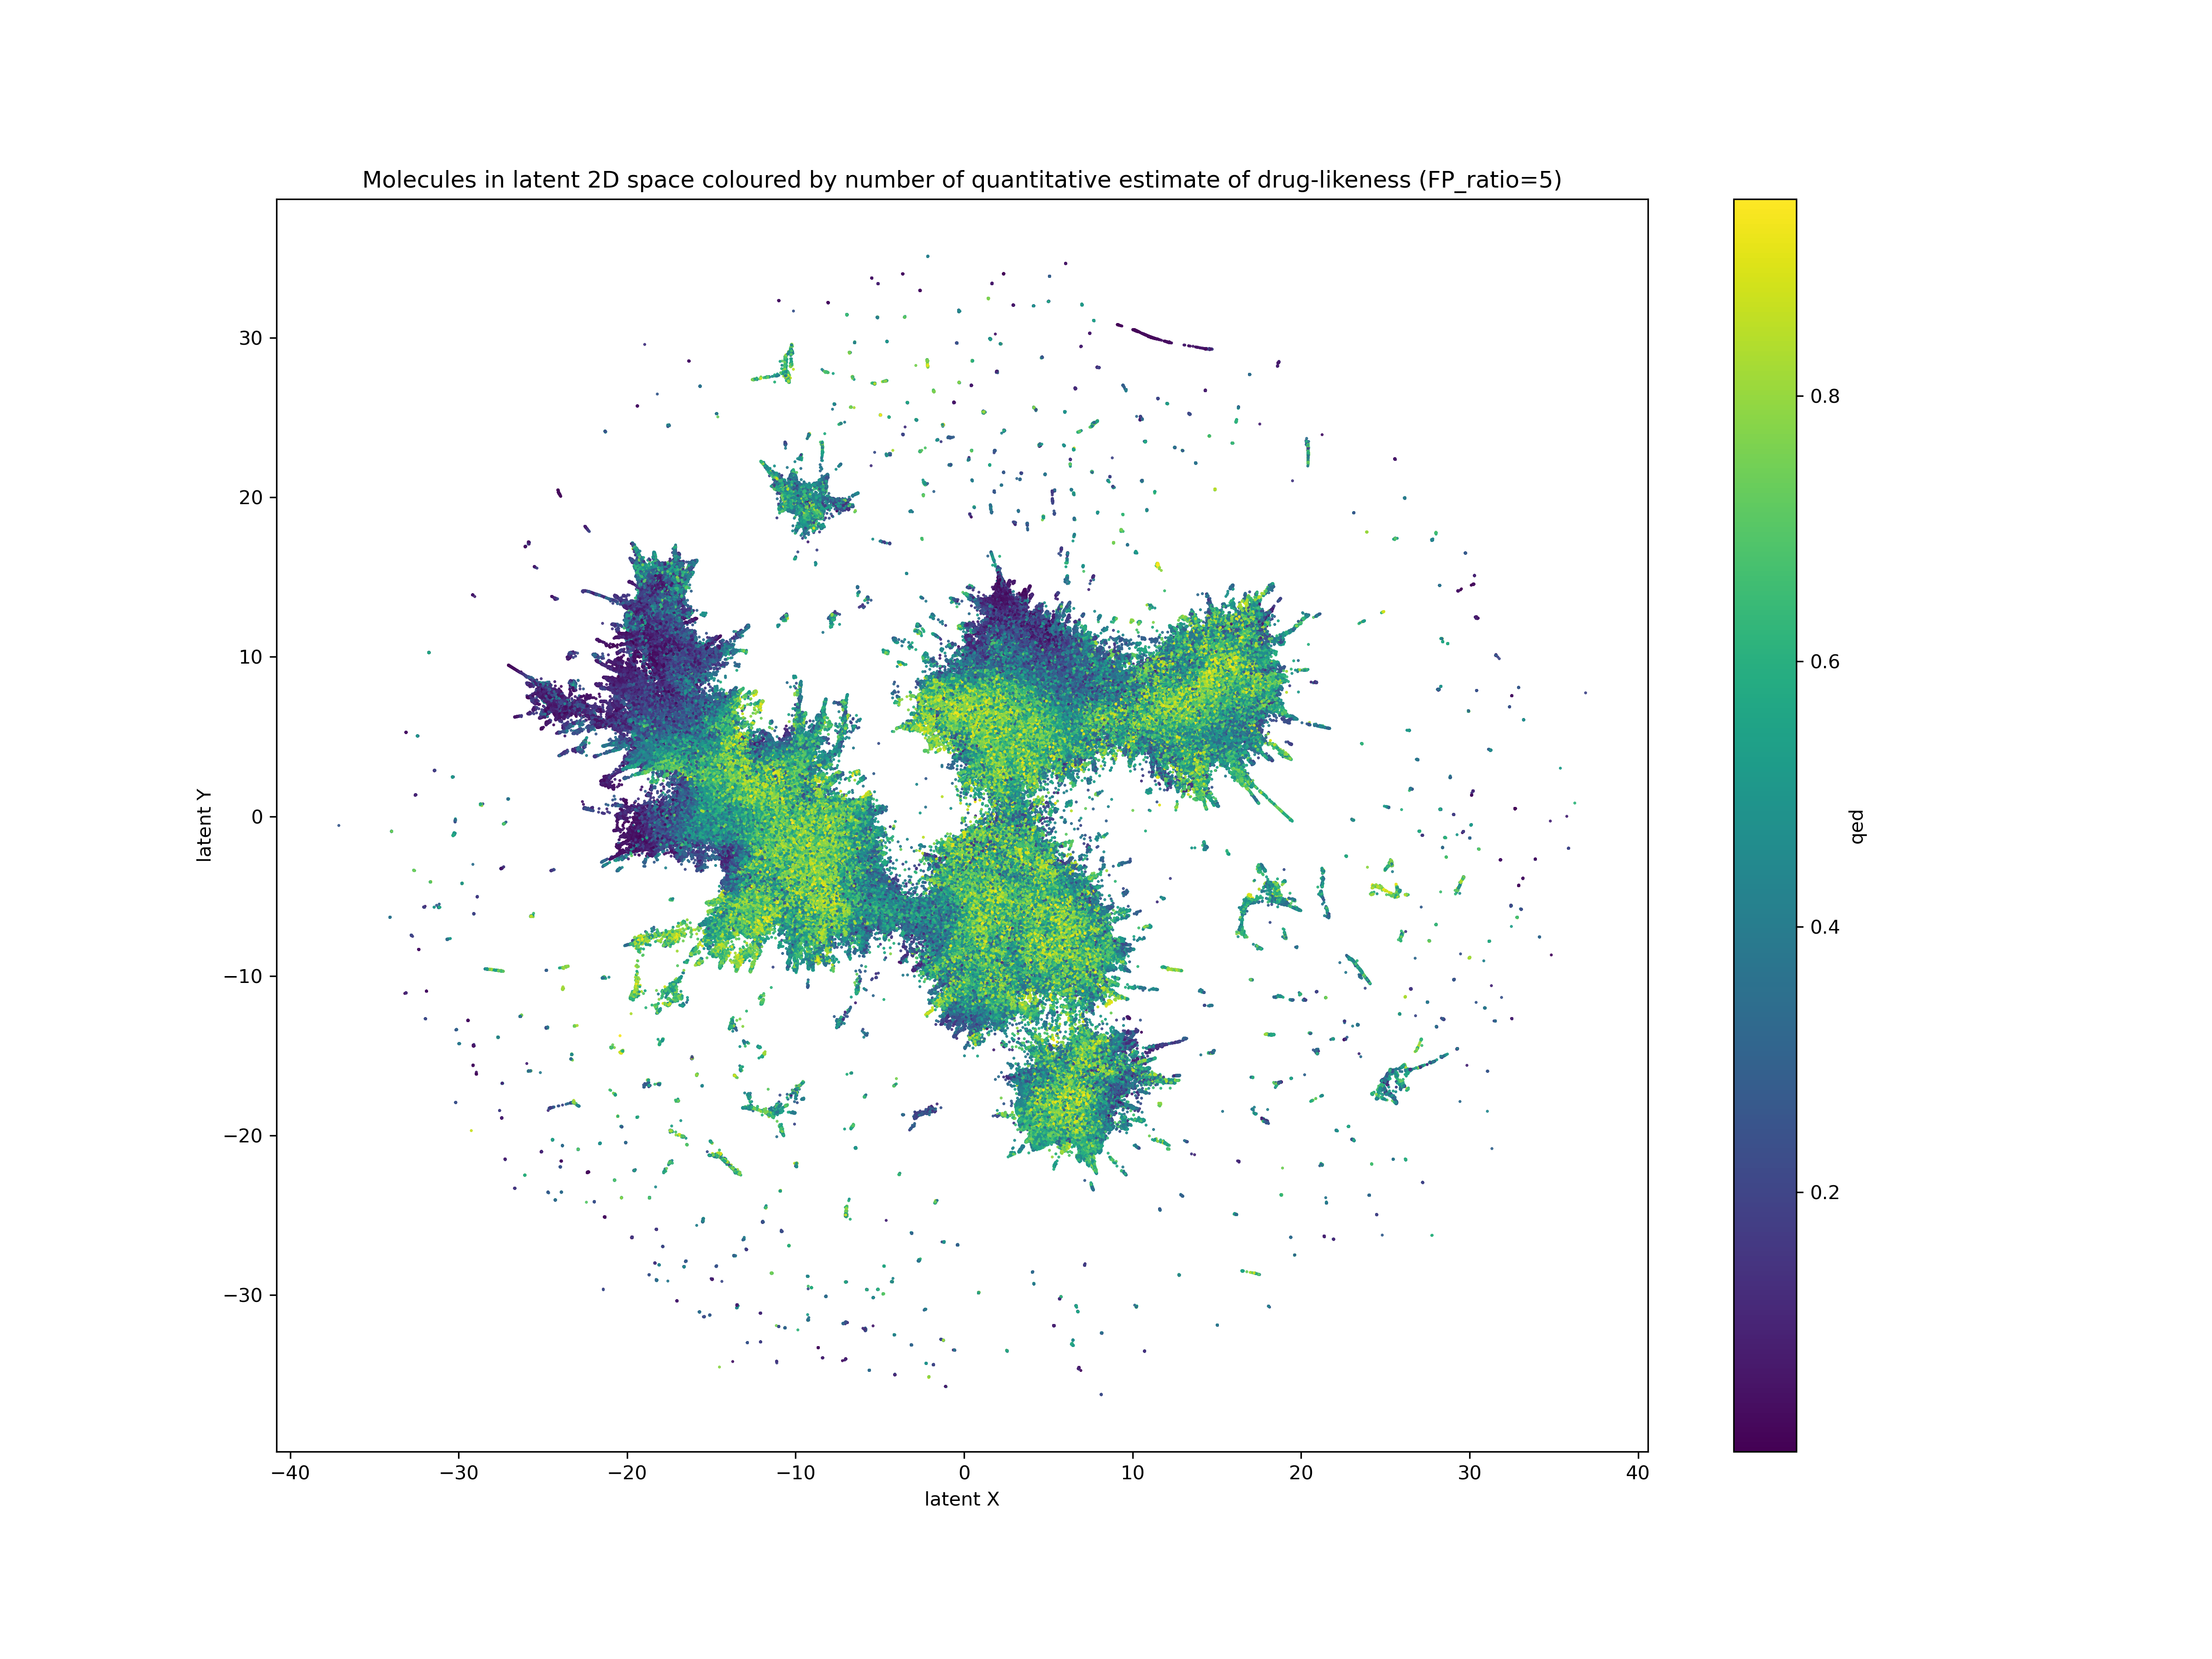
\includegraphics[width=0.45\columnwidth]{figures/PaCMAPqed@5}
	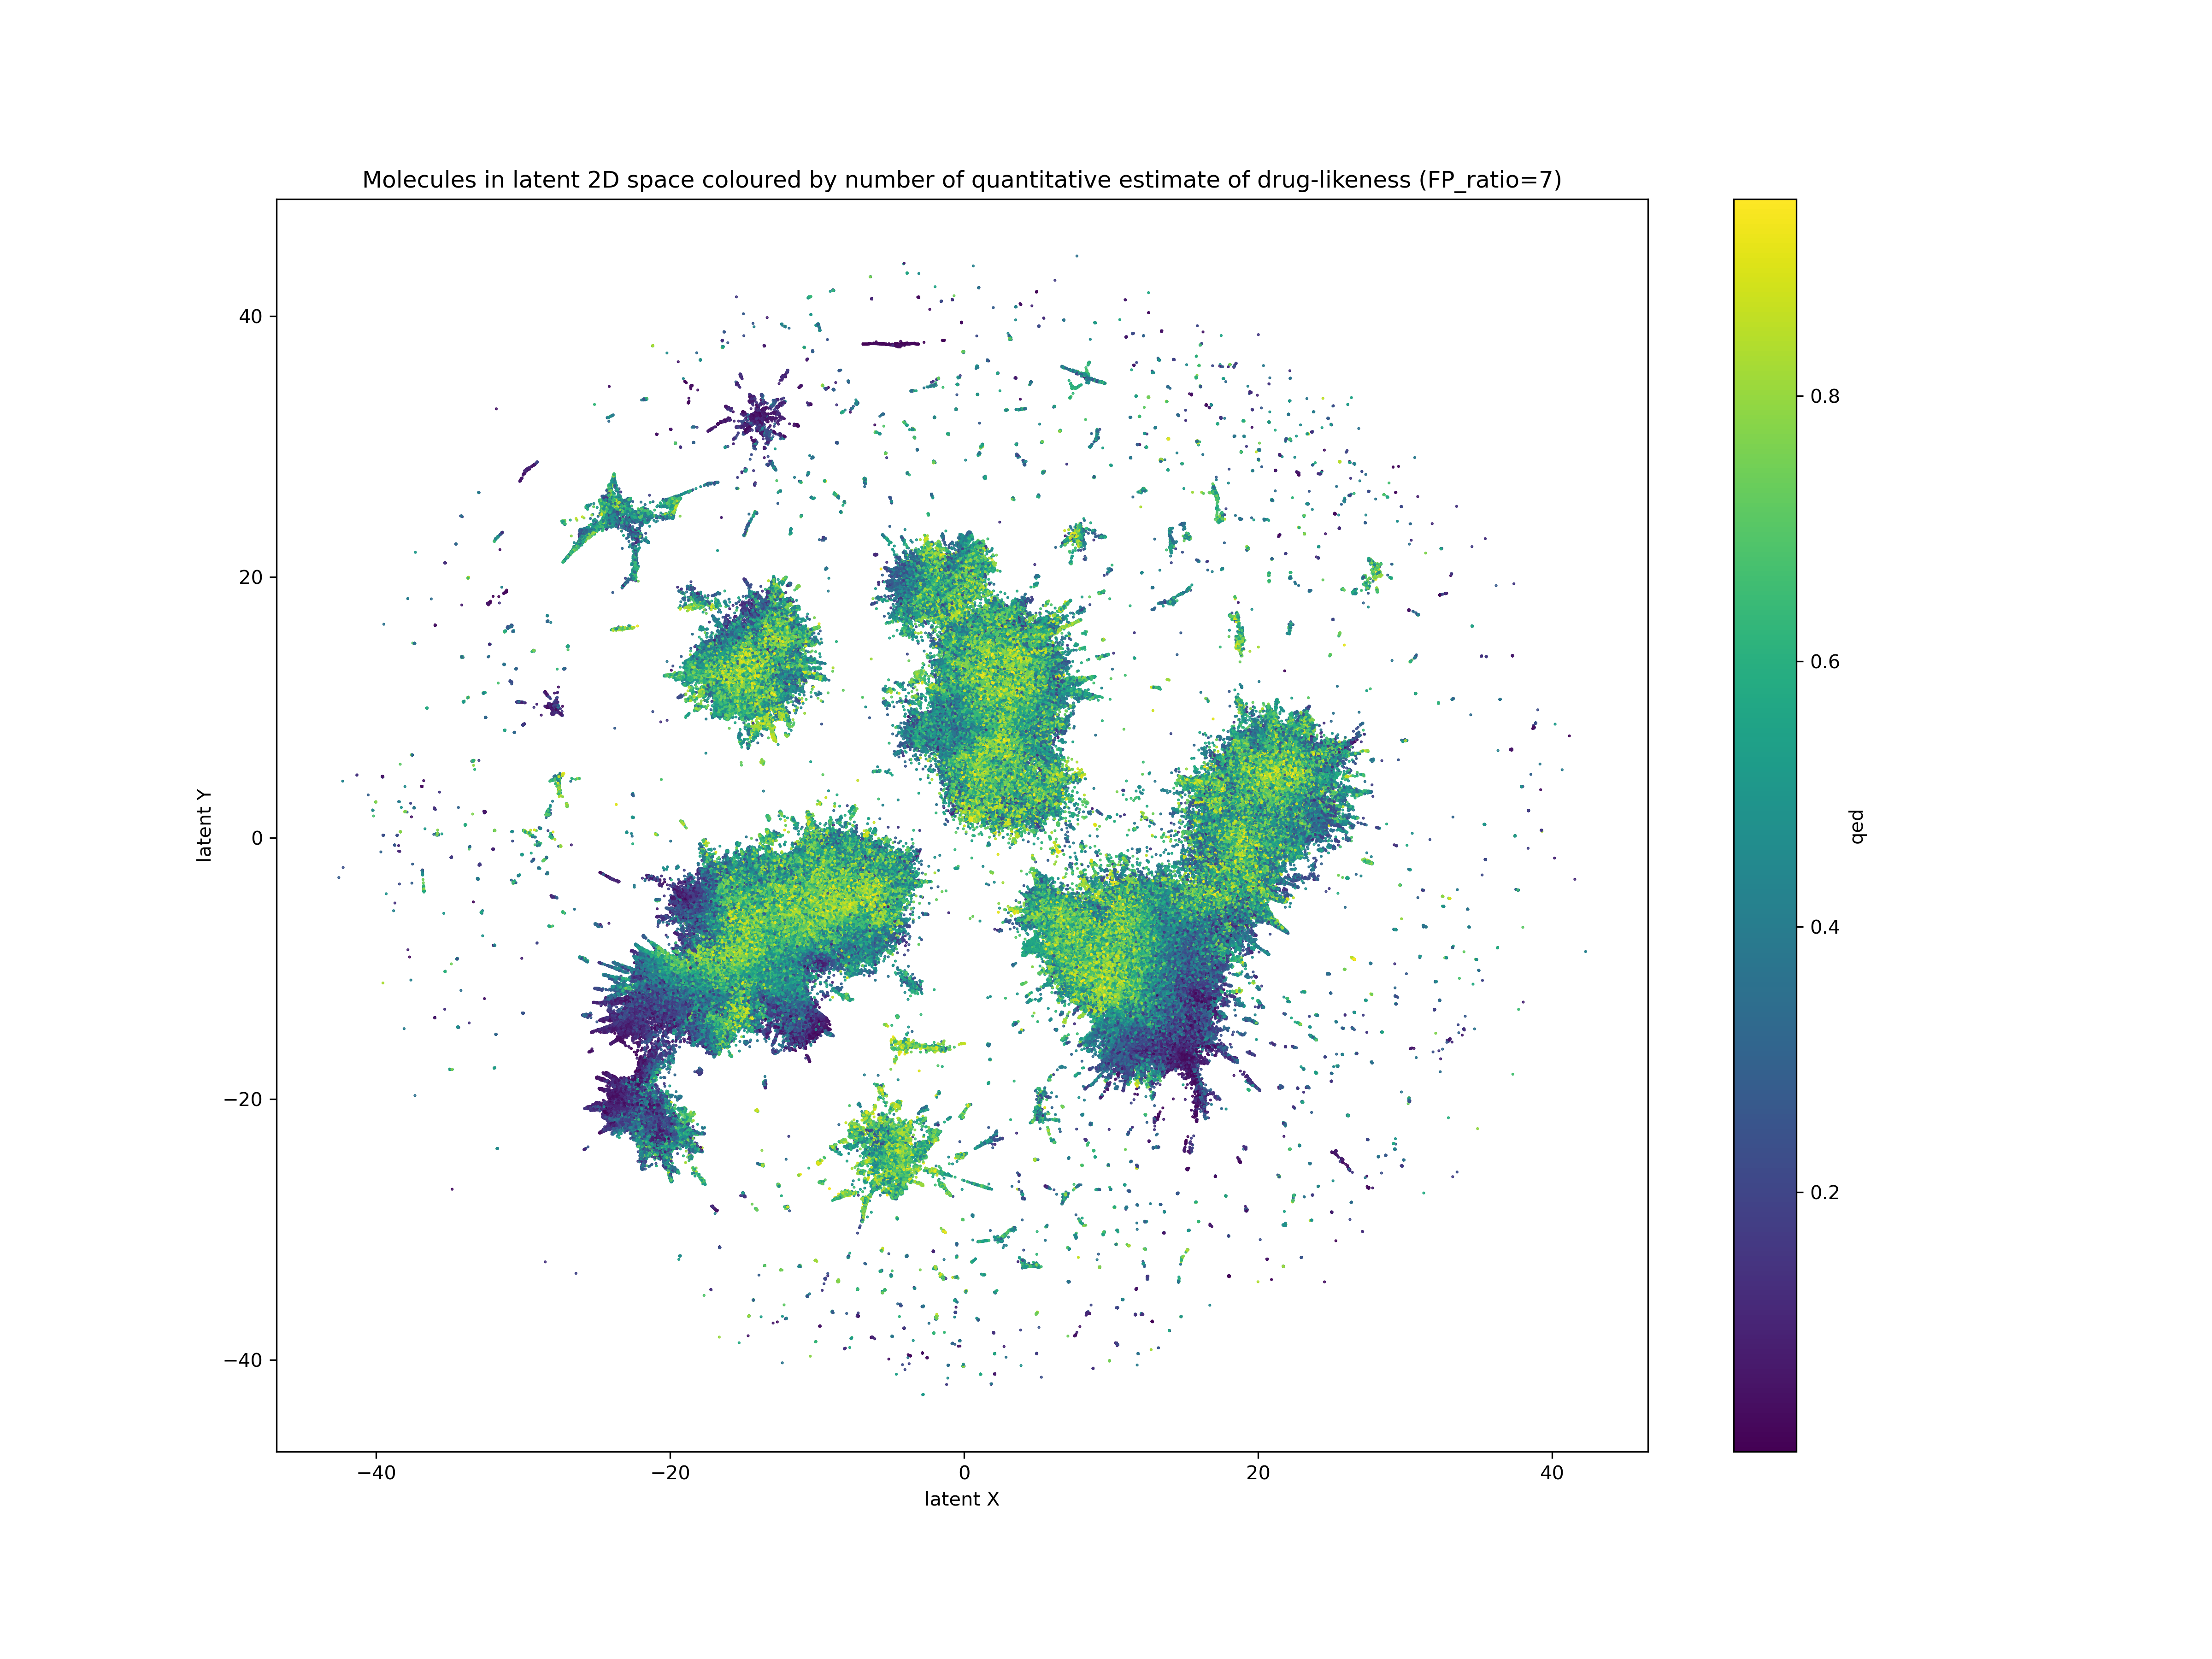
\includegraphics[width=0.45\columnwidth]{figures/PaCMAPqed@7}
	\includegraphics[width=0.45\columnwidth]{figures/PaCMAPqed@10}
	\caption{PaCMAP embeddings using various FP\_ratio parameters (0.5, 1, 3, 5, 7 and 10). Higher FP\_ratio resulted in more spread out clustering with less similar molecules close together. Tuning this parameter showed the most change out of all tested non-GD parameters.}
	\label{fig:pacmap:FP_ratio}
\end{figure}

With this in mind, I decided that the most important parameter to test was FP\_ratio, as it had the most effect on preserving local structure. I used many different values for the parameter, the result of some of which can be seen on figure (\ref{fig:pacmap:FP_ratio}). Clearly this hyperparameter has an immense effect on the result of PaCMAP. With larger values of FP\_ratio, the resulting space became more spread out, with distinct clusters forming. This is ideal for targeted searching, as the individual points are sorted into clusters based on similarity, pushing dissimilar point into other clusters.

It is important to note that this effect is not without drawbacks. As the FP\_ratio parameter increases, so does runtime. This relation is captured on table (\ref{tab:pacmap:runtime}). This is because the subset of data points used by PaCMAP increases as more further points are sampled for each observation.

\begin{table}
	\begin{center}
		\begin{tabular}{|c|r|}
			\hline
			FP\_ratio & Runtime (s)\\
			\hline 
			0.5 & 1:52:43.78 \\
			\hline
			7 & 7:14:07.76 \\
			\hline
			10 & 9:36:32.74 \\
			\hline
		\end{tabular}
	\end{center}
	\caption{The runtime of a few runs with different FP\_ratio parameters. There is a clear relation between the value and runtime. One should be careful setting extremely large values of this ratio.}
	\label{tab:pacmap:runtime}
\end{table}

\section{Overall results of hyperparameter optimization}\label{sec:overall-results-of-hyperparameter-optimization}

Overall, it can be said that these algorithms behave very differently when their parameters are tuned. While t-SNE does not significantly change its output with different values of perplexity, UMAP and PaCMAP both show major change with different parametrization. The potential of TriMAP is regrettably not known from this experiment.

The most potential comes with PaCMAP, as it has shifted the greatest amount from its default state. This however comes with a great increase of runtime. As for UMAP, while it has not shown as much tunability as PaCMAP, the fact that it runs much faster (with even GPU acceleration in certain implementations) can make it a more desirable method for common use. At this point, it seems like UMAP and PaCMAP are the most useful algorithms for \textit{de novo} molecule design.

\section{Linear interpolation test}\label{sec:linear-interpolation-test}

So far we have seen that each algorithm transformed the higher dimensional latent space in a way such that the formed clusters in which molecules shared similar properties. This does imply a smoothness over chemical structure in the output space, however, it does not mean that different clusters contain dissimilar molecules. The property of the output space that ensures the aggregation of all similar molecules into one cluster, while not essential, is very useful in \textit{de novo} molecule design, particularly in targeted searching.

In order to test the results of each algorithm for this property, I proposed a linear interpolation test, or LERP for short. This technique consists of selecting a fixed number of points that fit on a straight line between two selected observation in high dimension. These points are then added to the end of the dataset, and the new extended dataset is run through each algorithm. This results in a new embedding with those additional points that can be traced to see how the transition between data points are mapped to the output space.

There are many considerations needed to make with this kind of test. Firstly, the number of additional points may seem unimportant, however, it is one of the most important parameter. Choosing too many points relative to the size of the original dataset, the relations between the newly added points may overpower the underlying structure of the original dataset, transforming the embedding vastly. Choosing too few points however renders the test less useful, as the finer detail of the mapping is not seen. In my case, I chose the number of points to be 100, which is sufficiently small for the size of the dataset (1.6 million molecules) as to not change the overall topology of the embedding, while also enabling the finely detailed view of the mapping.

\begin{figure}[!h]
	\centering
	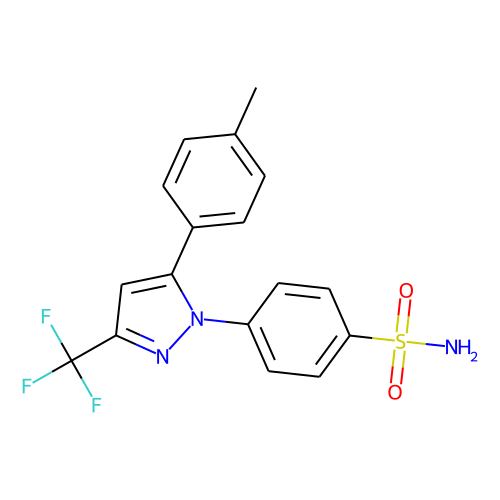
\includegraphics[width=0.4\columnwidth]{figures/coxib1}
	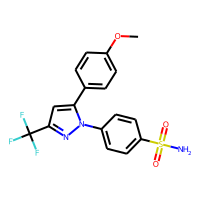
\includegraphics[width=0.4\columnwidth]{figures/coxib2}
	\caption{Two similar molecules (0.742 Tanimoto similarity) used in the linear interpolation test. The one on the left is celecoxib, a well-known COX-2 inhibitor. }
	\label{fig:coxib}
\end{figure}

The second parameter to consider is the choice of endpoints. Different choices of points lead to different insights learned by performing the test. By deliberately choosing similar points, one can examine whether similar points in the input space are truly mapped near each other in the output space. With a random selection, a more general trend can be observed. It shows the transition that the algorithm constructs between data points. The same can be said about deliberately choosing distant points, but that choice offers no more insight than the random point variant. In my test, I opted to try both similar molecules (figure (\ref{fig:coxib})) and random ones (figure (\ref{fig:random_mol})).

\begin{figure}[!h]
	\centering
	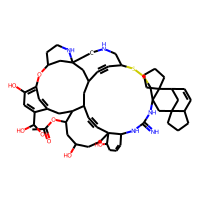
\includegraphics[width=0.4\columnwidth]{figures/random_mol1}
	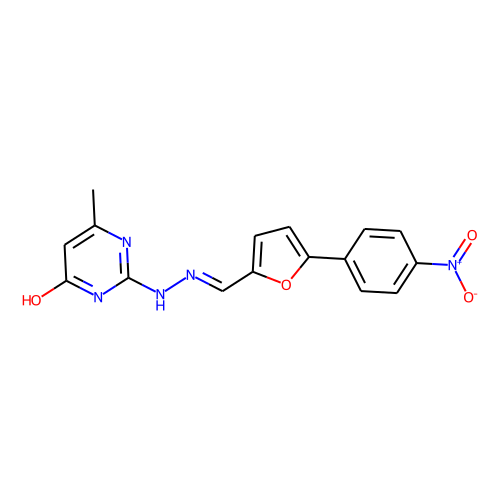
\includegraphics[width=0.4\columnwidth]{figures/random_mol2}
	\caption{Two randomly selected molecules that were used in the linear interpolation test. The two molecules have very distinctly different structures, and as such belong in different clusters.}
	\label{fig:random_mol}
\end{figure}

Finally, while I presented this test as a LERP, there are many other ways to sample points between two observations. On datasets with different topologies, different interpolation techniques work best. Particularly \textit{spherical linear interpolation} (SLERP) can be used as another useful method. In fact, during the training of the original autoencoder, SLERP was observed to give better results in novel molecule generation. \cite{bib:thesis} I have chosen to use LERP instead for conducting this test, as my use-case was not novel molecule sampling, and the mapping of a straight line is more interpretable as that of a circular arc.

If the mappings are not only smooth, but also relatively continuos, a curve of some kind should be drawn between the endpoints in two dimensions. With the similar molecules, it is also possible that the algorithms do not preserve the line topology, but instead transform the molecules into a cluster -- perhaps along with many other molecules. 

The first algorithm, PCA transformed the interpolations into straight lines, as seen on figure (\ref{fig:pca:lerp}). This is not surprising as PCA performs a linear transformation that maps straight lines into straight lines. It can be clearly seen that the similar molecules were transformed into points much closer on the plane than the random ones.

\begin{figure}[h]
	\centering
	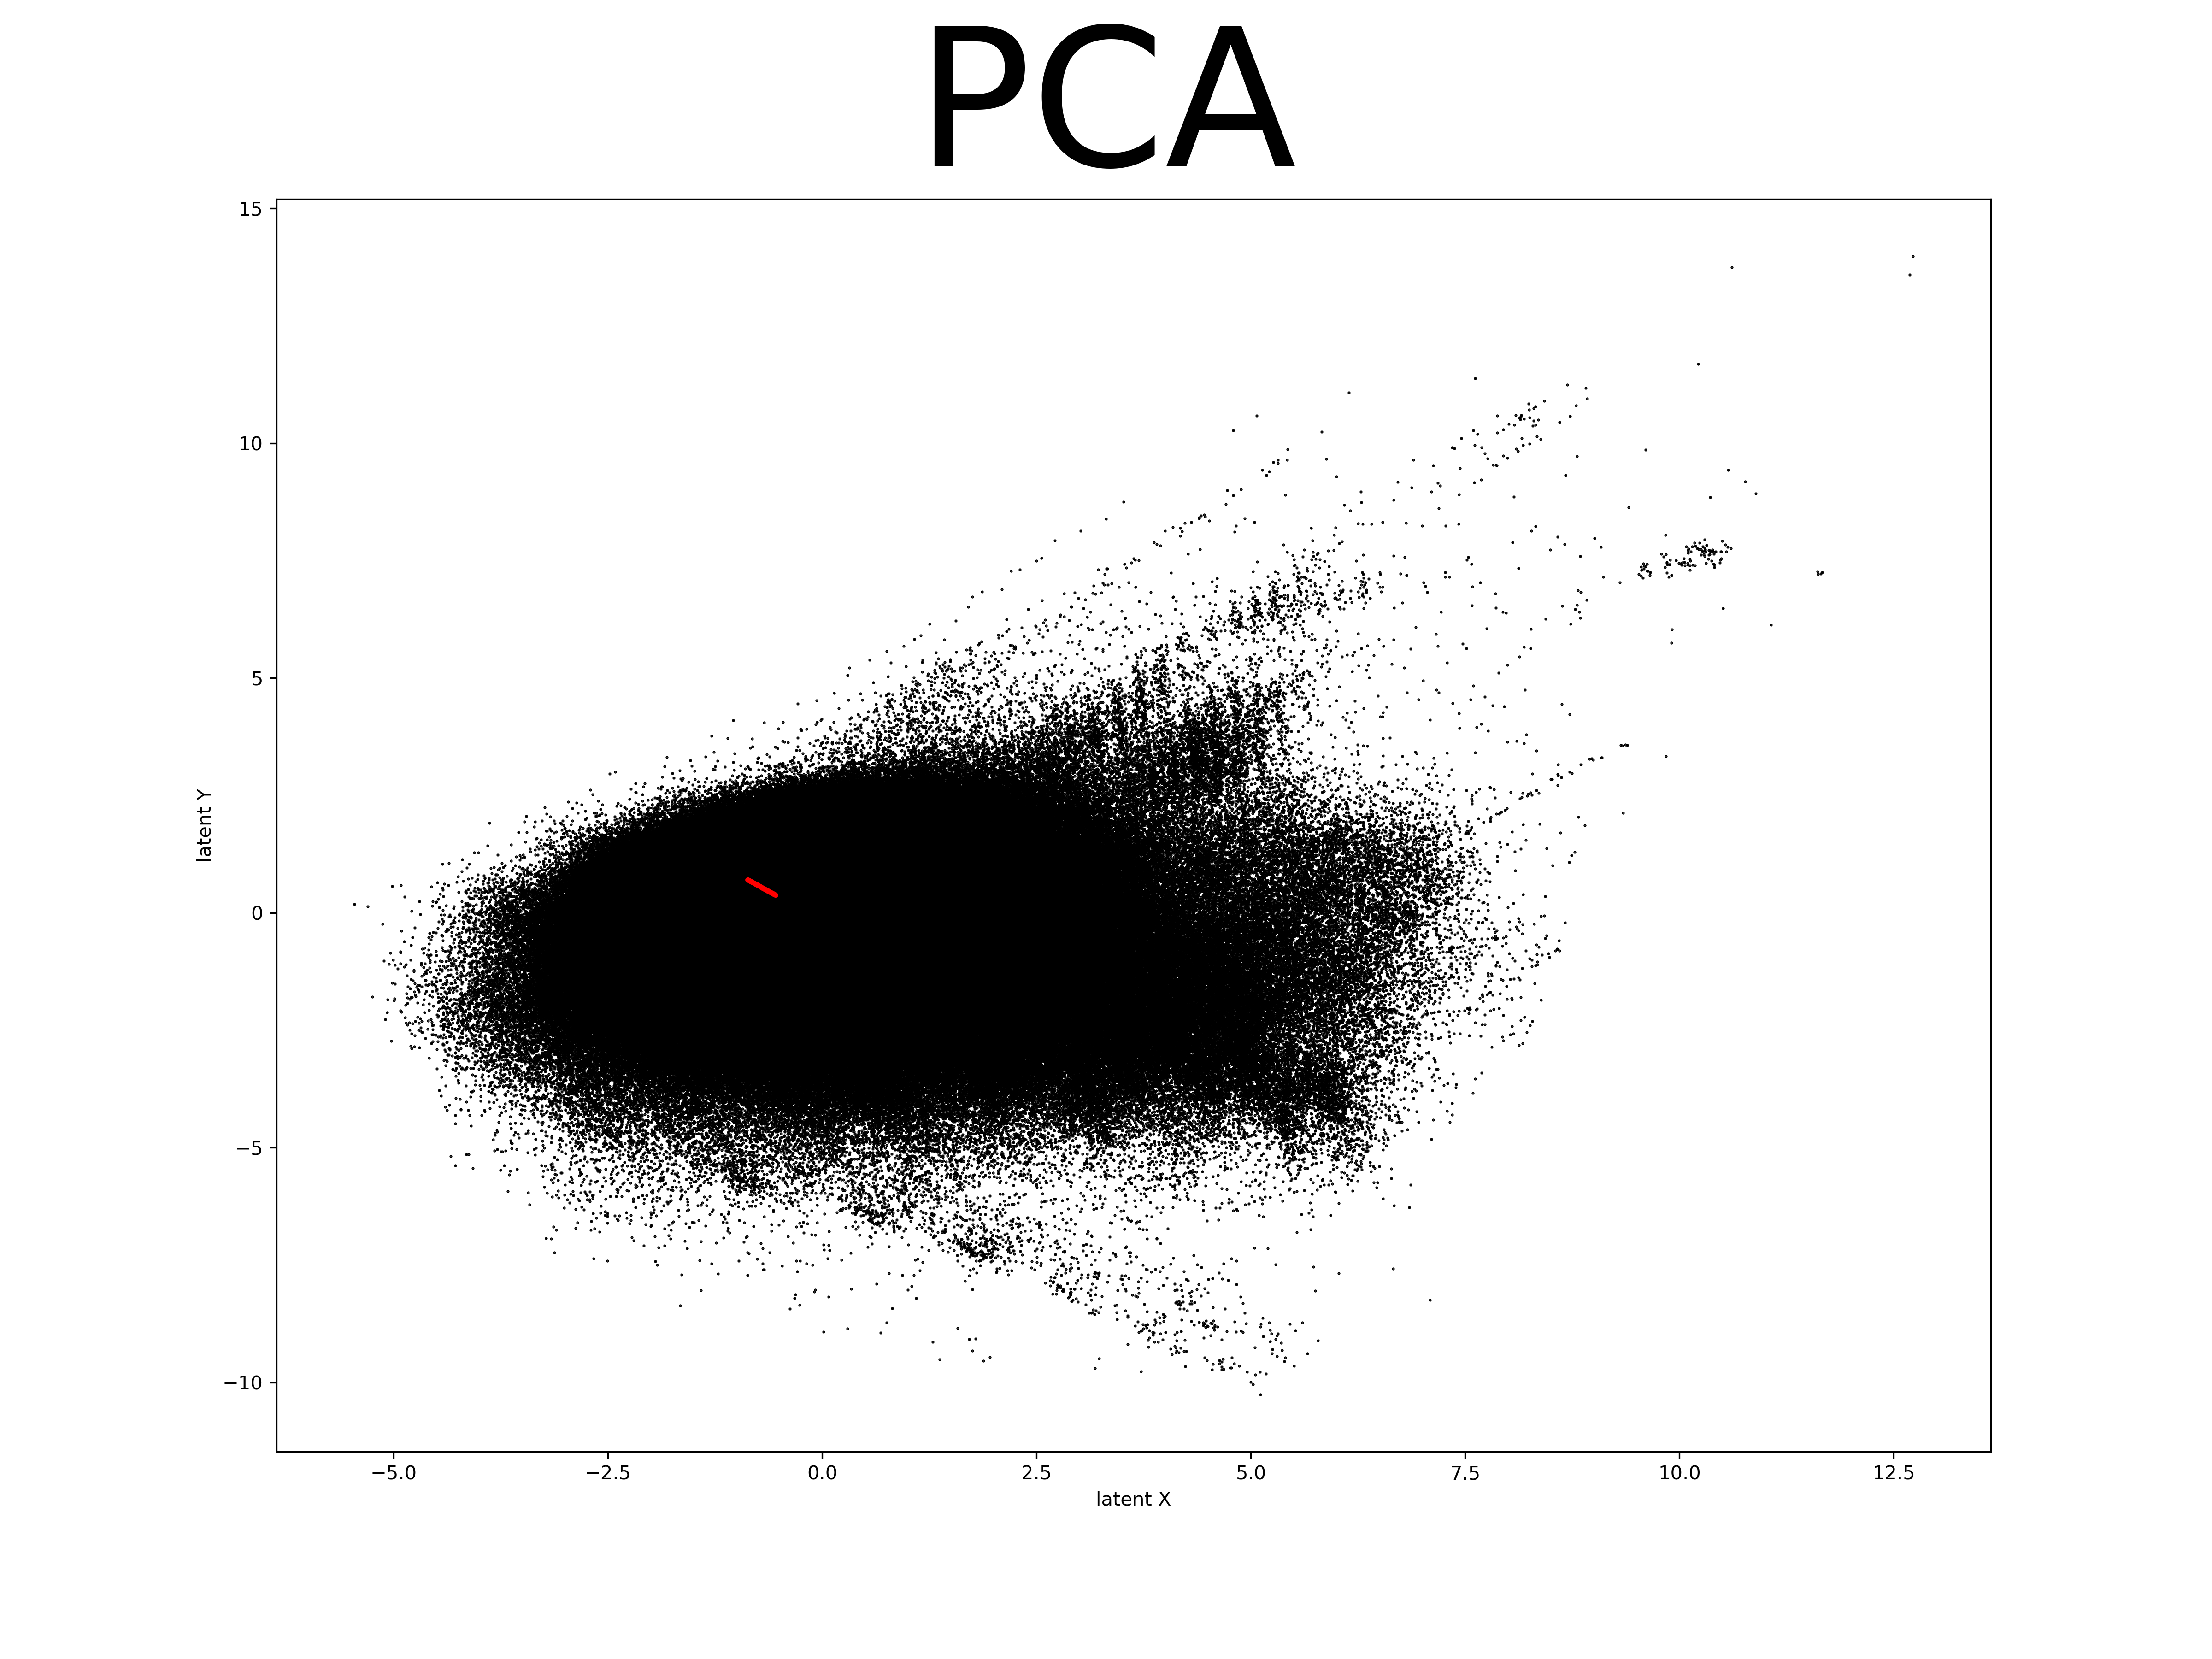
\includegraphics[width=0.49\columnwidth]{figures/PCA_LERP_coxib}
	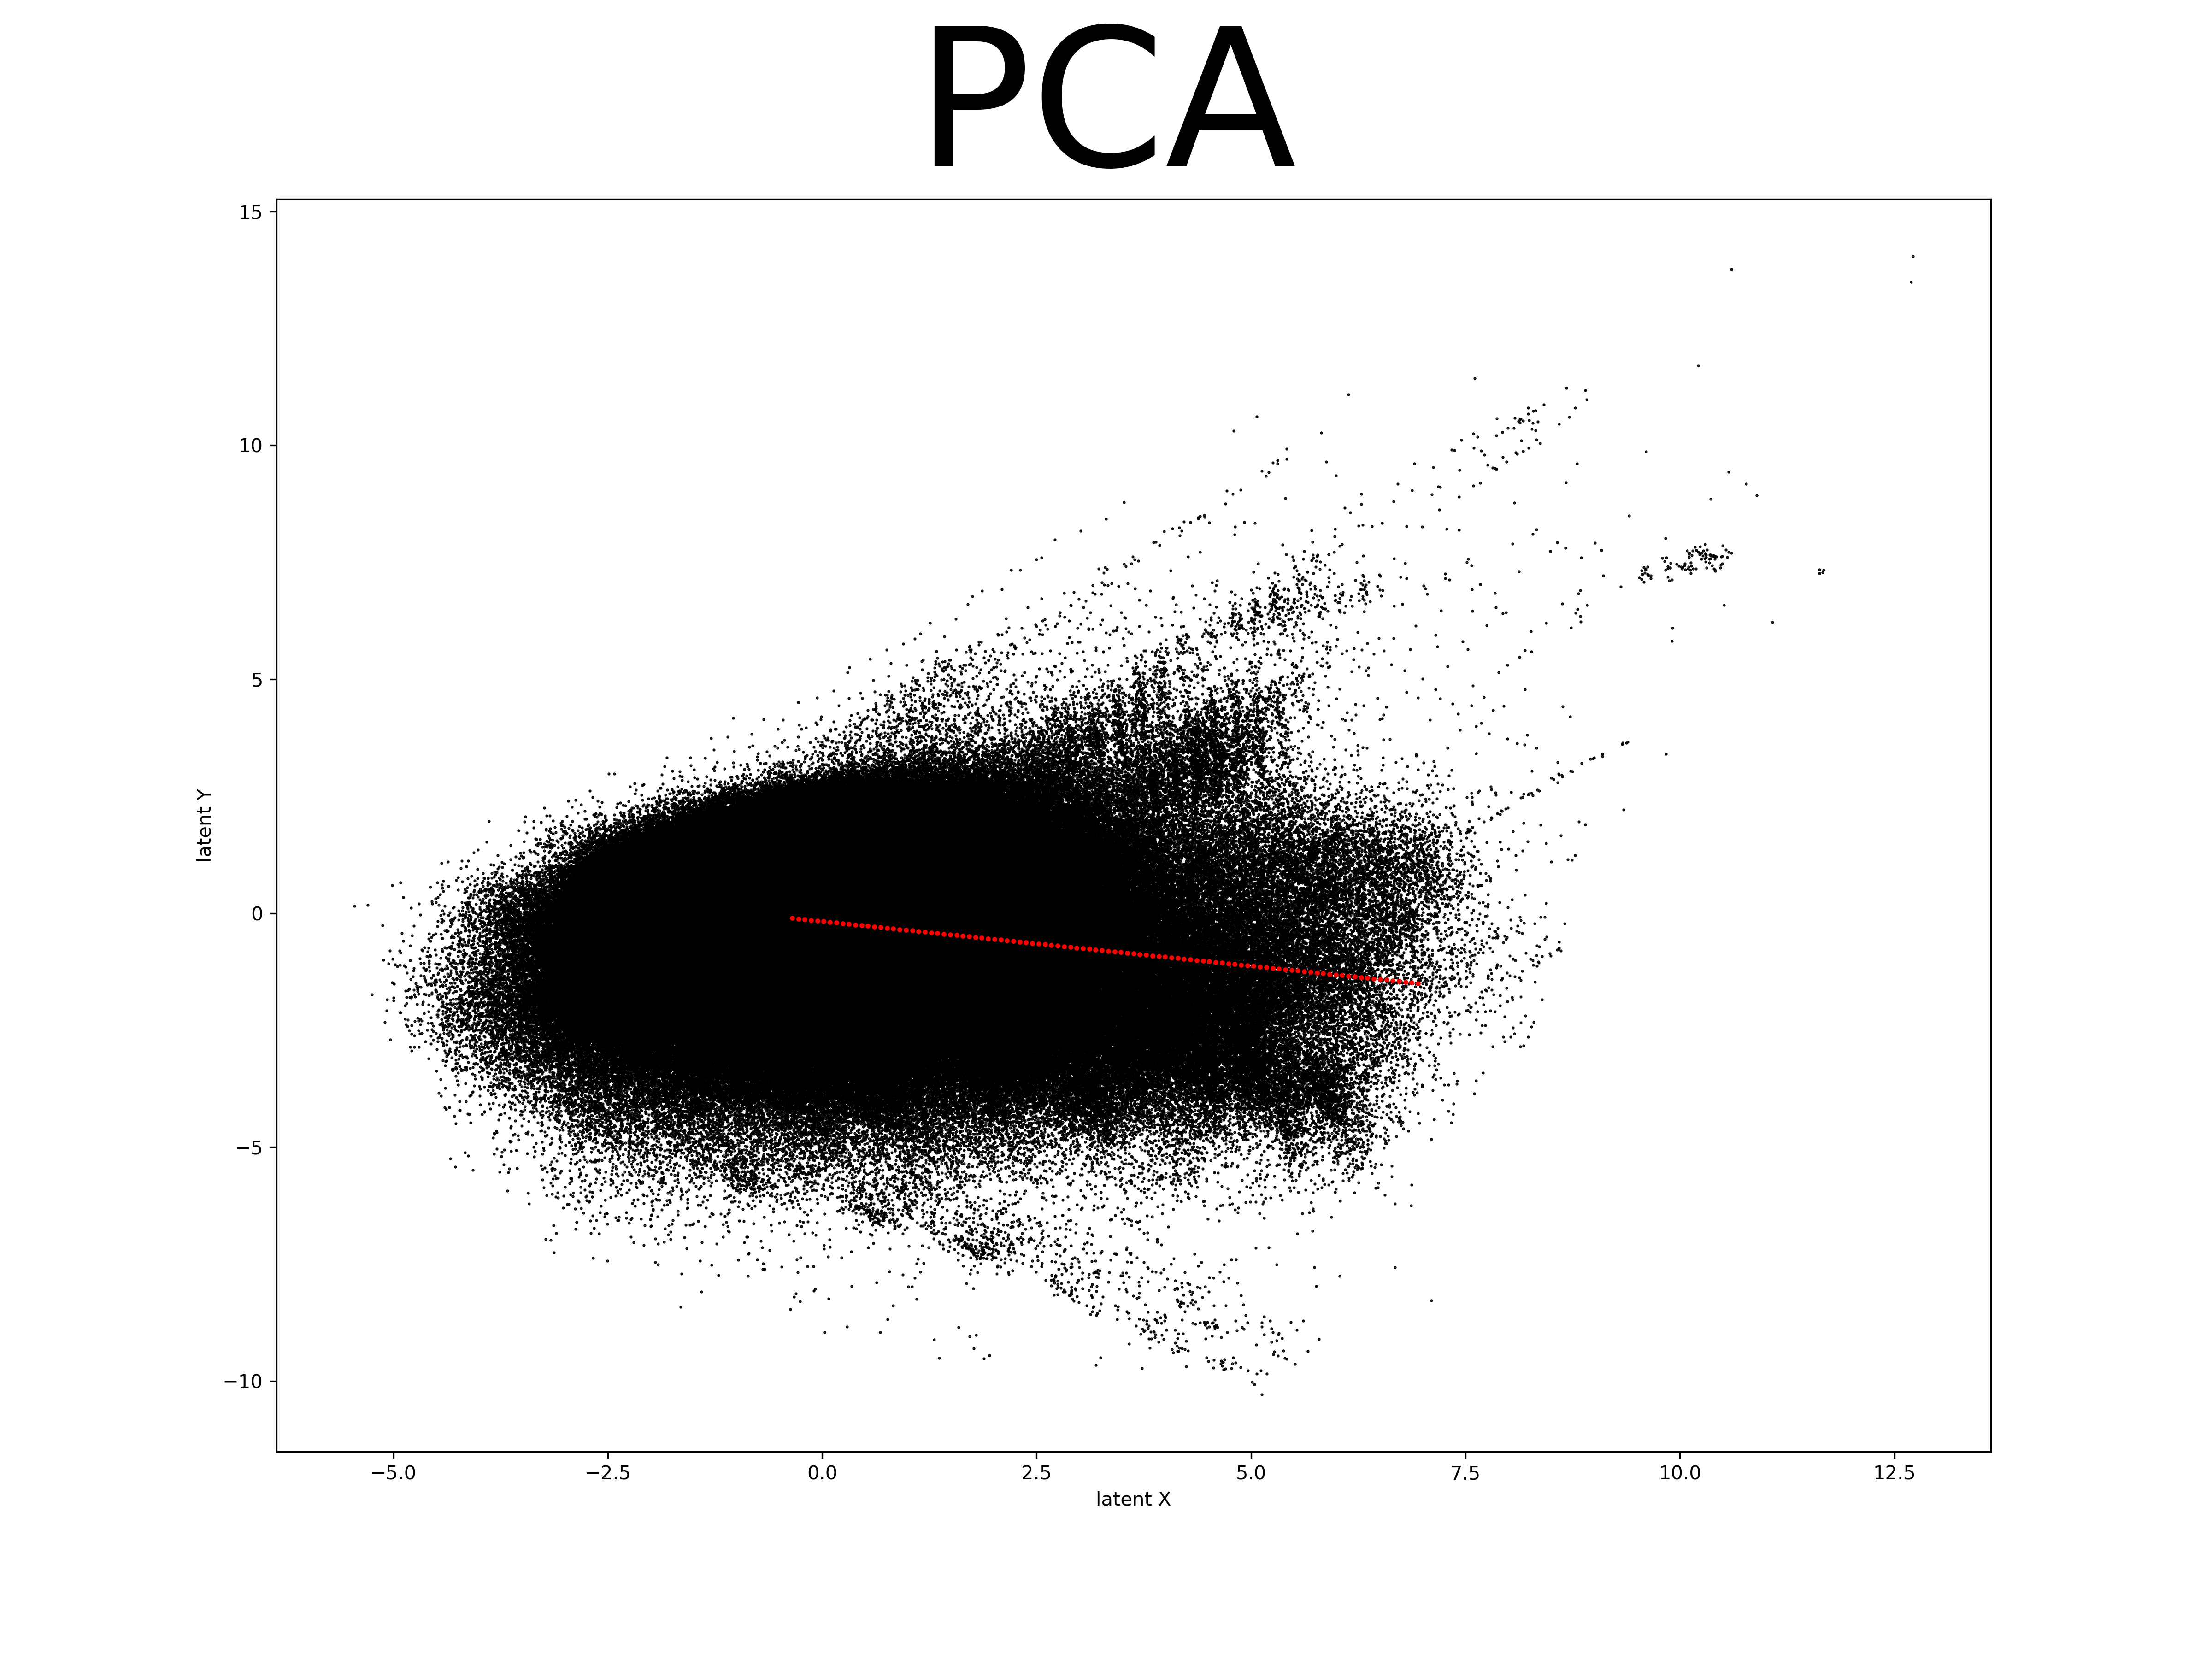
\includegraphics[width=0.49\columnwidth]{figures/PCA_LERP_random}
	\caption{Result of linear interpolation test of PCA with similar molecules (left) and random molecules (right). The shape of the trace line is straight.}
	\label{fig:pca:lerp}
\end{figure}

The results of t-SNE is significantly different than that of PCA. As can be seen on figure (\ref{fig:tsne:lerp}), t-SNE did not place the coxib molecules into the same cluster. Furthermore, the interpolated molecules are not placed in a curve between the two endpoints, rather placed into the clusters themselves. This results in a space where each point is surrounded by points that were close to it in the higher dimensional space. However, for targeted search, it is suboptimal, since many good candidate molecules are located in regions of the output space that is very far from the reference point.

\begin{figure}[h]
	\centering
	\includegraphics[width=0.5\columnwidth]{figures/t-SNE_LERP_coxib}
	\includegraphics[width=0.5\columnwidth]{figures/t-SNE_LERP_random}
	\caption{Result of linear interpolation test of t-SNE with similar molecules (left) and random molecules (right). In both cases, the chosen molecules were sorted into different clusters, and so were the interpolated points.}
	\label{fig:tsne:lerp}
\end{figure}

\todo{UMAP}

\begin{figure}[h]
	\centering
	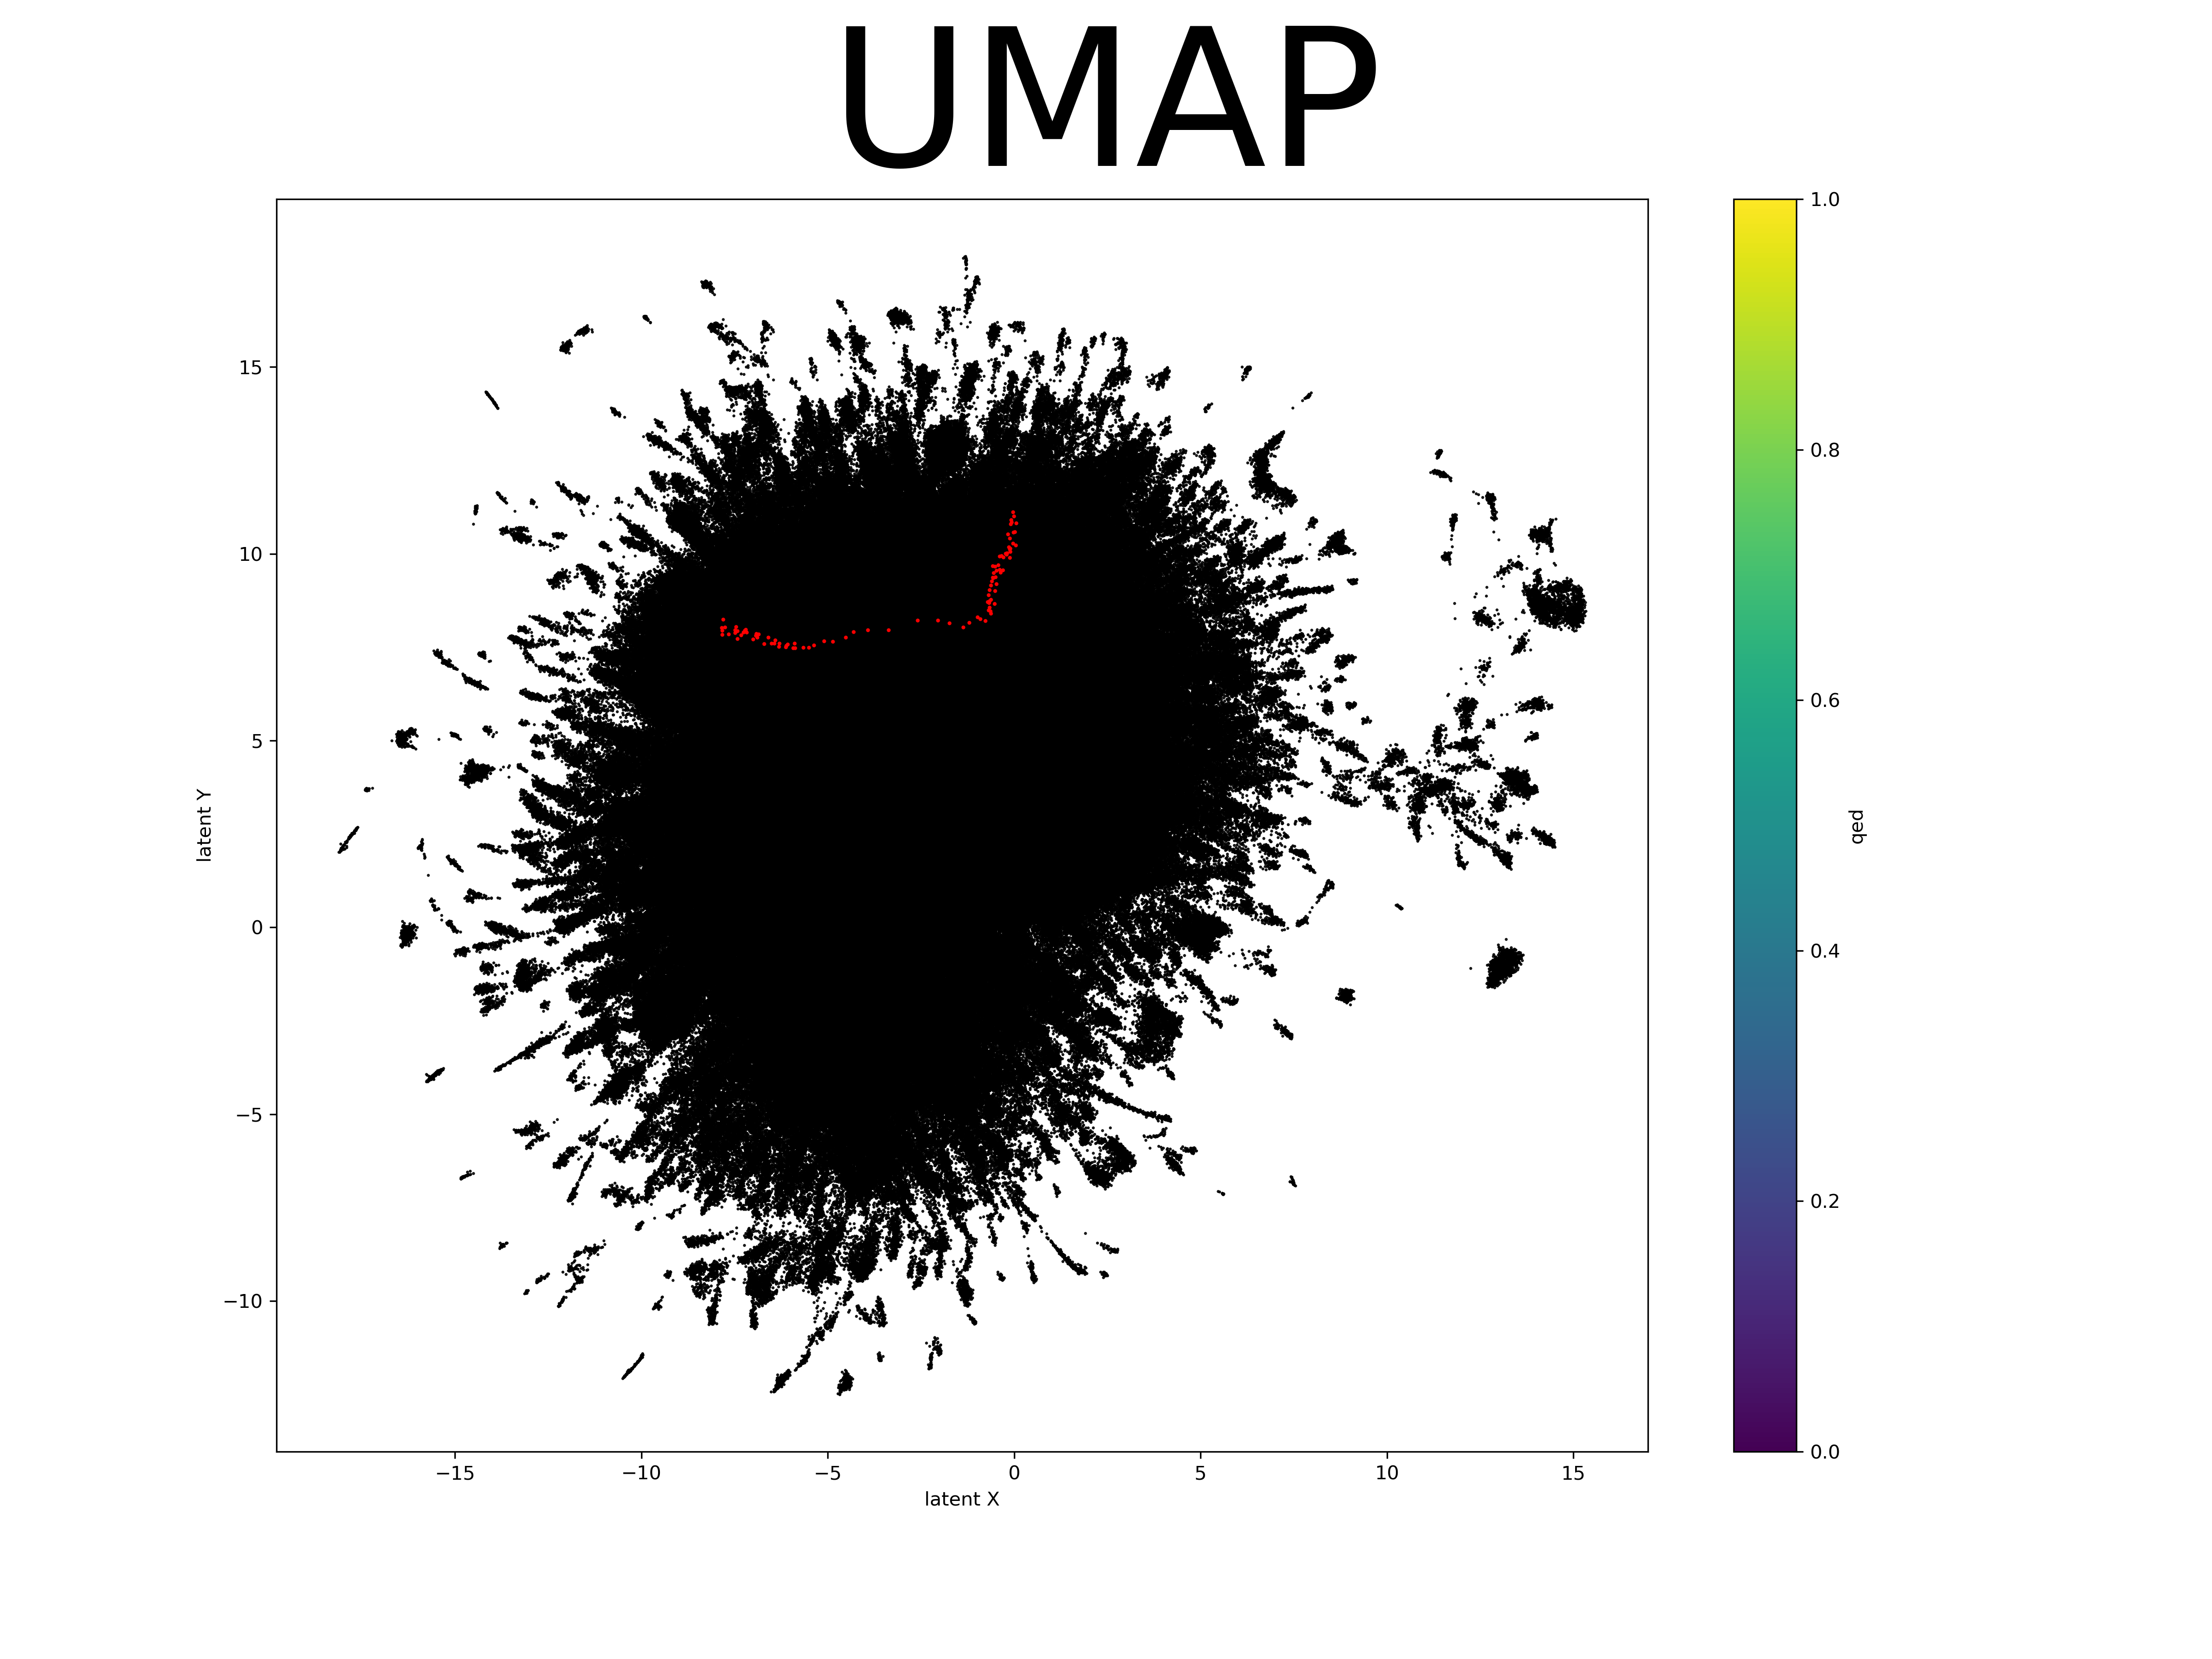
\includegraphics[width=0.5\columnwidth]{figures/UMAP_LERP_coxib}
	\includegraphics[width=0.5\columnwidth]{figures/UMAP_LERP_random}
	\caption{UMAP}
	\label{fig:umap:lerp}
\end{figure}

TriMAP resulted in the most unexpected embedding of all tested algorithms. The nature of the interpolated points were rather different than the others taken from embedding SMILES strings into a 64-dimensional latent space. This qualitative difference was picked up by TriMAP in both the tests. The algorithm placed the added points very far from all other points in two dimensions, as figure (\ref{fig:trimap:lerp}) shows. The rest of the input data was then embedded identically as without any added points. This shows how ``far-sighted'' TriMAP is. Even the difference between one hundred points on a line and 1.6 million points selected from a database embedded into a latent 64-dimensional space was enough to result in the total and perfect separation of the two classes.

\begin{figure}[h]
	\centering
	\includegraphics[width=0.7\columnwidth]{figures/TriMAP_LERP_coxib}
	\includegraphics[width=0.7\columnwidth]{figures/TriMAP_LERP_random}
	\caption{Linear interpolation test results made by TriMAP. In both cases (LERP between similar molecules on the left, random on the right), the algorithm separated the interpolated points very far from the rest of the dataset.}
	\label{fig:trimap:lerp}
\end{figure}

PaCMAP produced a result that could be described as expected. With an interpolation between two similar coxib molecules, the resulting embedding placed those extra points in one cluster, around the two endpoints. With random molecules however, the interpolation points were mapped to a line connecting two distinct clusters. These clusters were not too far apart, even though the two selected molecules possessed majorly different structures. This is possibly because the interpolated points connected the clusters, forcing PaCMAP to bring them closer to each other. This however did not result in the topology of the whole embedding to be different from normal runs. 

\begin{figure}[h]
	\centering
	\includegraphics[width=0.7\columnwidth]{figures/PaCMAP_LERP_coxib}
	\includegraphics[width=0.7\columnwidth]{figures/PaCMAP_LERP_random}
	\caption{PaCMAP embedding of the LERP tests. In the first case, the coxib-like points were all placed on the left of the space in one cluster. The randomly chosen LERP resulted on two clusters being connected on the right. No change to the topology of the whole embedding is observable.}
	\label{fig:pacmap:lerp}
\end{figure}


\begin{itemize}
	\item PCA made straight line, not surprising
	\item t-SNE split points into two clusters
	\item UMAP traced the path between them
	\item also has run where they aren't so far away
	\item TriMAP places new points very far away
	\item PaCMAP makes proper line
	\item with random points, it splits points into two clusters
	\item also has run where they are in one cluster
	\item UMAP has most promising results
\end{itemize}




%----------------------------------------------------------------------------
\chapter{Conclusion}\label{ch:conclusion}
%----------------------------------------------------------------------------


The main goal of this semester's work was to investigate the legitimacy of a number of different algorithms in the field of \textit{de novo} molecule design for reducing the dimension of a dataset in a meaningful way, allowing for targeted searching. I have learned much about each algorithm, and can confidently say which ones are particularly useful for this use-case and which ones are less so.

I have found that -- as many experts already know -- PCA is fundamentally unfit for such a task, as it has severe limitations in the correlations it can capture. t-SNE, which to this day is one of, if not the most popular dimension reduction algorithms, suffers from near-sightedness and performance issues both in terms of memory usage and runtime (the latter of which was not an issue because of the GPU implementation). UMAP seems to be among the most useful algorithms in this regard, transforming the chemical space in such a way as to be able to smoothly transition from one molecule to the next. In the tests, PaCMAP showed the most potential as the \textit{de facto}  go-to algorithm for pharmaceutical research. Unfortunately, the potential of TriMAP was not explored well enough for any definitive statement. However, educated guesses can be made to suggest that it is suboptimal for allowing targeted searching in its output space.

In the future, I would like to dive deeper into the optimal parametrization of each method. With more parameters to test, I believe a more desirable output space can be achieved with each method.

I would particularly like to test TriMAP more with the right parameters, because no conclusion can be made from the parameter optimization I performed.

While the LERP test was an important and fruitful examination of each algorithm's embedding quality, an arguably more important property of the implementation is the possibility of inverse transformation. That is, by sampling points from the output space, can a model return their respective positions in the original space. This would make targeted searching even more powerful, as one can simply search in the output space -- an operation that is faster because of the lowered dimensionality -- and produce the corresponding molecules by inverse transforming the sampled dataset.

Overall, the work I have done this semester answers quite a few questions about the validity of such dimension reduction algorithms in \textit{de novo} molecule design, but there are still more to investigate.
%----------------------------------------------------------------------------
\chapter{A dolgozat formai kivitele}
%----------------------------------------------------------------------------
Az itt található információk egy része a BME VIK Hallgatói Képviselet által készített ,,Utolsó félév a villanykaron'' c. munkából lett kis változtatásokkal átemelve. Az eredeti dokumentum az alábbi linken érhető el: \url{http://vik.hk/hirek/diplomafelev-howto-2015}.

%----------------------------------------------------------------------------
\section{A dolgozat kimérete}
%----------------------------------------------------------------------------
Szakdolgozat esetében minimum 30, 45 körüli ajánlott oldalszám lehet az iránymutató. De mindenképp érdemes rákérdezni a konzulensnél is az elvárásokra, mert tanszékenként változóak lehetnek az elvárások.

Mesterképzésen a Diplomatervezés 1 esetében a beszámoló még inkább az Önálló laboratóriumi beszámolókhoz hasonlít, tanszékenként eltérő formai követelményekkel, -- egy legalább 30 oldal körüli dolgozat az elvárt -- és az elmúlt fél éves munkáról szól. De egyben célszerű, ha ez a végleges diplomaterv alapja is. (A végleges 60-90 oldal körülbelül a hasznos részre nézve)


%----------------------------------------------------------------------------
\section{A dolgozat nyelve}
%----------------------------------------------------------------------------
Mivel Magyarországon a hivatalos nyelv a magyar, ezért alapértelmezésben magyarul kell megírni a dolgozatot. Aki külföldi posztgraduális képzésben akar részt venni, nemzetközi szintű tudományos kutatást szeretne végezni, vagy multinacionális cégnél akar elhelyezkedni, annak célszerű angolul megírnia diplomadolgozatát. Mielőtt a hallgató az angol nyelvű verzió mellett dönt, erősen ajánlott mérlegelni, hogy ez mennyi többletmunkát fog a hallgatónak jelenteni fogalmazás és nyelvhelyesség terén, valamint -- nem utolsó sorban -- hogy ez mennyi többletmunkát fog jelenteni a konzulens illetve bíráló számára. Egy nehezen olvasható, netalán érthetetlen szöveg teher minden játékos számára.

%----------------------------------------------------------------------------
\section{A dokumentum nyomdatechnikai kivitele}
%----------------------------------------------------------------------------
A dolgozatot A4-es fehér lapra nyomtatva, 2,5 centiméteres margóval (+1~cm kötésbeni), 11--12 pontos betűmérettel, talpas betűtípussal és másfeles sorközzel célszerű elkészíteni.

Annak érdekében, hogy a dolgozat külsőleg is igényes munka benyomását keltse, érdemes figyelni az alapvető tipográfiai szabályok betartására.



% Acknowledgements
%~~~~~~~~~~~~~~~~~~~~~~~~~~~~~~~~~~~~~~~~~~~~~~~~~~~~~~~~~~~~~~~~~~~~~~~~~~~~~~~~~~~~~~
% \include{content/acknowledgement}


% List of Figures, Tables
%~~~~~~~~~~~~~~~~~~~~~~~~~~~~~~~~~~~~~~~~~~~~~~~~~~~~~~~~~~~~~~~~~~~~~~~~~~~~~~~~~~~~~~
%\listoffigures\addcontentsline{toc}{chapter}{\listfigurename}
%\listoftables\addcontentsline{toc}{chapter}{\listtablename}


% Bibliography
%~~~~~~~~~~~~~~~~~~~~~~~~~~~~~~~~~~~~~~~~~~~~~~~~~~~~~~~~~~~~~~~~~~~~~~~~~~~~~~~~~~~~~~
\addcontentsline{toc}{chapter}{\bibname}
\bibliography{bib/mybib}


% Appendix
%~~~~~~~~~~~~~~~~~~~~~~~~~~~~~~~~~~~~~~~~~~~~~~~~~~~~~~~~~~~~~~~~~~~~~~~~~~~~~~~~~~~~~~
%----------------------------------------------------------------------------
\appendix
%----------------------------------------------------------------------------
\chapter*{\fuggelek}\addcontentsline{toc}{chapter}{\fuggelek}
\setcounter{chapter}{\appendixnumber}
%\setcounter{equation}{0} % a fofejezet-szamlalo az angol ABC 6. betuje (F) lesz
\numberwithin{equation}{section}
\numberwithin{figure}{section}
\numberwithin{lstlisting}{section}
%\numberwithin{tabular}{section}

%----------------------------------------------------------------------------
\section{Exact packages used}
%----------------------------------------------------------------------------

\begin{table}
	\begin{center}
		\begin{tabular}{|l|r|r|l|}
			 \textbf{Name} &\textbf{Version} &\textbf{Build} &\textbf{Channel} \\
			 \hline
			\_libgcc\_mutex &0.1 & conda\_forge &conda-forge \\
			\_openmp\_mutex &4.5 & 1\_gnu &conda-forge \\
			\_tflow\_select &2.1.0 & gpu & \\
			absl-py &0.11.0 & py37h89c1867\_0 &conda-forge \\
			annoy &1.17.0 & pypi\_0 &pypi \\
			argon2-cffi &20.1.0 & pypi\_0 &pypi \\
			astor &0.8.1 & pyh9f0ad1d\_0 &conda-forge \\
			async-generator &1.10 & pypi\_0 &pypi \\
			attrs &20.3.0 & pypi\_0 &pypi \\
			backcall &0.2.0 & pypi\_0 &pypi \\
			binutils\_impl\_linux-64 &2.35.1 & h193b22a\_2 &conda-forge \\
			binutils\_linux-64 &2.35 & h67ddf6f\_30 &conda-forge \\
			blas &1.0 & openblas & \\
			bleach &3.3.0 & pypi\_0 &pypi \\
			boost &1.74.0 & py37h6dcda5c\_3 &conda-forge \\
			boost-cpp &1.74.0 & hc6e9bd1\_2 &conda-forge \\
			bzip2 &1.0.8 & h7f98852\_4 &conda-forge \\
			c-ares &1.17.1 & h36c2ea0\_0 &conda-forge \\
			ca-certificates &2020.12.5 & ha878542\_0 &conda-forge \\
			cached-property &1.5.1 & py\_0 &conda-forge \\
			cairo &1.16.0 & h7979940\_1007 &conda-forge \\
			certifi &2020.12.5 & py37h89c1867\_1 &conda-forge \\
			cffi &1.14.5 & pypi\_0 &pypi \\
			cuda100 &1.0 & hb0b9368\_0 &cannylab \\
			cudatoolkit &10.0.130 & hf841e97\_8 &conda-forge \\
			cudnn &7.6.5.32 & ha8d7eb6\_1 &conda-forge \\
			cupti &10.0.130 & 0 & \\
			cycler &0.10.0 & py\_2 &conda-forge \\
			dbus &1.13.6 & hfdff14a\_1 &conda-forge \\
			decorator &4.4.2 & pypi\_0 &pypi \\
			defusedxml &0.6.0 & pypi\_0 &pypi \\
			entrypoints &0.3 & pypi\_0 &pypi \\
			expat &2.3.0 & h9c3ff4c\_0 &conda-forge \\
			fcd &1.1 & pyh9f0ad1d\_0 &conda-forge \\
			ffmpeg &4.3.1 & hca11adc\_2 &conda-forge \\
			fontconfig &2.13.1 & hba837de\_1004 &conda-forge \\
			freetype &2.10.4 & h0708190\_1 &conda-forge \\
			gast &0.2.2 & py\_0 &conda-forge \\
			
		\end{tabular}
	\end{center}
\end{table}

\begin{table}
	\begin{center}
		\begin{tabular}{|l|r|r|l|}
			\textbf{Name} &\textbf{Version} &\textbf{Build} &\textbf{Channel} \\
			\hline
			gcc\_impl\_linux-64 &9.3.0 & h70c0ae5\_18 &conda-forge \\
			gcc\_linux-64 &9.3.0 & hf25ea35\_30 &conda-forge \\
			gettext &0.19.8.1 & h0b5b191\_1005 &conda-forge \\
			glib &2.66.7 & h9c3ff4c\_0 &conda-forge \\
			glib-tools &2.66.7 & h9c3ff4c\_0 &conda-forge \\
			gmp &6.2.1 & h58526e2\_0 &conda-forge \\
			gnutls &3.6.13 & h85f3911\_1 &conda-forge \\
			google-pasta &0.2.0 & pyh8c360ce\_0 &conda-forge \\
			graphite2 &1.3.13 & h58526e2\_1001 &conda-forge \\
			grpcio &1.36.0 & py37hb27c1af\_0 &conda-forge \\
			gst-plugins-base &1.18.4 & h29181c9\_0 &conda-forge \\
			gstreamer &1.18.4 & h76c114f\_0 &conda-forge \\
			guacamol &0.5.2 & pyh9f0ad1d\_0 &conda-forge \\
			gxx\_impl\_linux-64 &9.3.0 & hd87eabc\_18 &conda-forge \\
			gxx\_linux-64 &9.3.0 & h3fbe746\_30 &conda-forge \\
			h5py &3.1.0 & nompi\_py37h1e651dc\_100 &conda-forge \\
			harfbuzz &2.8.0 & h83ec7ef\_0 &conda-forge \\
			hdf5 &1.10.6 & hb1b8bf9\_0 & \\
			icu &68.1 & h58526e2\_0 &conda-forge \\
			importlib-metadata &3.7.0 & py37h89c1867\_0 &conda-forge \\
			ipykernel &5.5.0 & pypi\_0 &pypi \\
			ipython &7.21.0 & pypi\_0 &pypi \\
			ipython-genutils &0.2.0 & pypi\_0 &pypi \\
			ipywidgets &7.6.3 & pypi\_0 &pypi \\
			jasper &1.900.1 & h07fcdf6\_1006 &conda-forge \\
			jedi &0.18.0 & pypi\_0 &pypi \\
			jinja2 &2.11.3 & pypi\_0 &pypi \\
			joblib &1.0.1 & pyhd8ed1ab\_0 &conda-forge \\
			jpeg &9d & h36c2ea0\_0 &conda-forge \\
			jsonschema &3.2.0 & pypi\_0 &pypi \\
			jupyter &1.0.0 & pypi\_0 &pypi \\
			jupyter-client &6.1.11 & pypi\_0 &pypi \\
			jupyter-console &6.2.0 & pypi\_0 &pypi \\
			jupyter-core &4.7.1 & pypi\_0 &pypi \\
			jupyterlab-pygments &0.1.2 & pypi\_0 &pypi \\
			jupyterlab-widgets &1.0.0 & pypi\_0 &pypi \\
			keras &2.3.1 & py37\_0 &conda-forge \\
			keras-applications &1.0.8 & py\_1 &conda-forge \\
			keras-preprocessing &1.1.2 & pyhd8ed1ab\_0 &conda-forge \\
			kernel-headers\_linux-64 &2.6.32 & h77966d4\_13 &conda-forge \\
			kiwisolver &1.3.1 & py37h2527ec5\_1 &conda-forge \\
			krb5 &1.17.2 & h926e7f8\_0 &conda-forge \\
			lame &3.100 & h7f98852\_1001 &conda-forge \\
			lcms2 &2.12 & hddcbb42\_0 &conda-forge \\
			ld\_impl\_linux-64 &2.35.1 & hea4e1c9\_2 &conda-forge \\
			libblas &3.8.0 & 17\_openblas &conda-forge \\
			libcblas &3.8.0 & 17\_openblas &conda-forge \\
			libclang &11.1.0 & default\_ha53f305\_0 & conda-forge \\
			libcurl &7.71.1 & hcdd3856\_8 &conda-forge \\
			libedit &3.1.20191231 & he28a2e2\_2 &conda-forge \\
				
		\end{tabular}
	\end{center}
\end{table}			


\begin{table}
	\begin{center}
		\begin{tabular}{|l|r|r|l|}
			\textbf{Name} &\textbf{Version} &\textbf{Build} &\textbf{Channel} \\
			\hline
			libev &4.33 & h516909a\_1 &conda-forge \\
			libevent &2.1.10 & hcdb4288\_3 &conda-forge \\
			libffi &3.3 & h58526e2\_2 &conda-forge \\
			libgcc-devel\_linux-64 &9.3.0 & h7864c58\_18 &conda-forge \\
			libgcc-ng &9.3.0 & h2828fa1\_18 &conda-forge \\
			libgfortran-ng &7.3.0 & hdf63c60\_0 & \\
			libglib &2.66.7 & h1f3bc88\_0 &conda-forge \\
			libgomp &9.3.0 & h2828fa1\_18 &conda-forge \\
			libgpuarray &0.7.6 & h7f98852\_1003 &conda-forge \\
			libiconv &1.16 & h516909a\_0 &conda-forge \\
			liblapack &3.8.0 & 17\_openblas &conda-forge \\
			liblapacke &3.8.0 & 17\_openblas &conda-forge \\
			libllvm11 &11.1.0 & hf817b99\_2 &conda-forge \\
			libnghttp2 &1.43.0 & h812cca2\_0 &conda-forge \\
			libopenblas &0.3.10 & h5a2b251\_0 & \\
			libopencv &4.5.1 & py37h90094e2\_0 &conda-forge \\
			libpng &1.6.37 & h21135ba\_2 &conda-forge \\
			libpq &13.2 & hfd2b0eb\_2 &conda-forge \\
			libprotobuf &3.15.2 & h780b84a\_0 &conda-forge \\
			libssh2 &1.9.0 & hab1572f\_5 &conda-forge \\
			libstdcxx-devel\_linux-64 &9.3.0 & hb016644\_18 &conda-forge \\
			libstdcxx-ng &9.3.0 & h6de172a\_18 &conda-forge \\
			libtiff &4.2.0 & hdc55705\_0 &conda-forge \\
			libuuid &2.32.1 & h7f98852\_1000 &conda-forge \\
			libwebp-base &1.2.0 & h7f98852\_0 &conda-forge \\
			libxcb &1.13 & h7f98852\_1003 &conda-forge \\
			libxkbcommon &1.0.3 & he3ba5ed\_0 &conda-forge \\
			libxml2 &2.9.10 & h72842e0\_3 &conda-forge \\
			llvmlite &0.37.0 & pypi\_0 &pypi \\
			lz4-c &1.9.3 & h9c3ff4c\_0 &conda-forge \\
			mako &1.1.4 & pyh44b312d\_0 &conda-forge \\
			markdown &3.3.4 & pyhd8ed1ab\_0 &conda-forge \\
			markupsafe &1.1.1 & py37h5e8e339\_3 &conda-forge \\
			matplotlib-base &3.3.4 & py37h0c9df89\_0 &conda-forge \\
			mistune &0.8.4 & pypi\_0 &pypi \\
			mysql-common &8.0.23 & ha770c72\_1 &conda-forge \\
			mysql-libs &8.0.23 & h935591d\_1 &conda-forge \\
			nbclient &0.5.3 & pypi\_0 &pypi \\
			nbconvert &6.0.7 & pypi\_0 &pypi \\
			nbformat &5.1.2 & pypi\_0 &pypi \\
			ncurses &6.2 & h58526e2\_4 &conda-forge \\
			nest-asyncio &1.5.1 & pypi\_0 &pypi \\
			nettle &3.6 & he412f7d\_0 &conda-forge \\
			nomkl &3.0 & 0 & \\
			notebook &6.2.0 & pypi\_0 &pypi \\
			nspr &4.30 & h9c3ff4c\_0 &conda-forge \\
			nss &3.63 & hb5efdd6\_0 &conda-forge \\
			numba &0.54.0 & pypi\_0 &pypi \\
			numpy &1.20.3 & pypi\_0 &pypi \\
			olefile &0.46 & pyh9f0ad1d\_1 &conda-forge \\
			
		\end{tabular}
	\end{center}
\end{table}		


\begin{table}
	\begin{center}
		\begin{tabular}{|l|r|r|l|}
			\textbf{Name} &\textbf{Version} &\textbf{Build} &\textbf{Channel} \\
			\hline
			openblas &0.3.10 & 0 & \\
			openblas-devel &0.3.10 & 0 & \\
			opencv &4.5.1 & py37h89c1867\_0 &conda-forge \\
			openh264 &2.1.1 & h780b84a\_0 &conda-forge \\
			openssl &1.1.1k & h7f98852\_0 &conda-forge \\
			opentsne &0.5.2 & py37hda21425\_0 &conda-forge \\
			opt\_einsum &3.3.0 & py\_0 &conda-forge \\
			packaging &20.9 & pypi\_0 &pypi \\
			pacmap &0.3 & pypi\_0 &pypi \\
			pandas &1.2.2 & py37hdc94413\_0 &conda-forge \\
			pandocfilters &1.4.3 & pypi\_0 &pypi \\
			parso &0.8.1 & pypi\_0 &pypi \\
			pcre &8.44 & he1b5a44\_0 &conda-forge \\
			pexpect &4.8.0 & pypi\_0 &pypi \\
			pickleshare &0.7.5 & pypi\_0 &pypi \\
			pillow &8.1.0 & py37h4600e1f\_2 &conda-forge \\
			pip &21.0.1 & pyhd8ed1ab\_0 &conda-forge \\
			pixman &0.40.0 & h36c2ea0\_0 &conda-forge \\
			prometheus-client &0.9.0 & pypi\_0 &pypi \\
			prompt-toolkit &3.0.16 & pypi\_0 &pypi \\
			protobuf &3.15.2 & py37hcd2ae1e\_0 &conda-forge \\
			pthread-stubs &0.4 & h36c2ea0\_1001 &conda-forge \\
			ptyprocess &0.7.0 & pypi\_0 &pypi \\
			py-opencv &4.5.1 & py37h888b3d9\_0 &conda-forge \\
			pycairo &1.20.0 & py37h01af8b0\_1 &conda-forge \\
			pycparser &2.20 & pypi\_0 &pypi \\
			pygments &2.8.0 & pypi\_0 &pypi \\
			pygpu &0.7.6 & py37h902c9e0\_1002 & conda-forge \\
			pynndescent &0.5.4 & pypi\_0 &pypi \\
			pyparsing &2.4.7 & pyh9f0ad1d\_0 &conda-forge \\
			pyrsistent &0.17.3 & pypi\_0 &pypi \\
			python &3.7.10 & hffdb5ce\_100\_cpython &conda-forge \\
			python-dateutil &2.8.1 & py\_0 &conda-forge \\
			python\_abi &3.7 & 1\_cp37m &conda-forge \\
			pytz &2021.1 & pyhd8ed1ab\_0 &conda-forge \\
			pyyaml &5.4.1 & py37h5e8e339\_0 &conda-forge \\
			pyzmq &22.0.3 & pypi\_0 &pypi \\
			qt &5.12.9 & hda022c4\_4 &conda-forge \\
			qtconsole &5.0.2 & pypi\_0 &pypi \\
			qtpy &1.9.0 & pypi\_0 &pypi \\
			rdkit &2020.09.4 & py37he53b9e1\_0 &conda-forge \\
			readline &8.0 & he28a2e2\_2 &conda-forge \\
			reportlab &3.5.60 & py37h69800bb\_0 &conda-forge \\
			scikit-learn &0.24.1 & py37h69acf81\_0 &conda-forge \\
			scipy &1.6.1 & py37hf56f3a7\_0 & \\
			send2trash &1.5.0 & pypi\_0 &pypi \\
			setuptools &49.6.0 & py37h89c1867\_3 &conda-forge \\
			six &1.15.0 & pyh9f0ad1d\_0 &conda-forge \\
			sqlalchemy &1.3.23 & py37h5e8e339\_0 &conda-forge \\
			sqlite &3.34.0 & h74cdb3f\_0 &conda-forge \\
			
		\end{tabular}
	\end{center}
\end{table}	

\begin{table}
	\begin{center}
		\begin{tabular}{|l|r|r|l|}
			\textbf{Name} &\textbf{Version} &\textbf{Build} &\textbf{Channel} \\
			\hline
			sysroot\_linux-64 &2.12 & h77966d4\_13 &conda-forge \\
			tensorboard &1.15.0 & py37\_0 &conda-forge \\
			tensorflow &1.15.0 & gpu\_py37h0f0df58\_0 & \\
			tensorflow-base &1.15.0 & gpu\_py37h9dcbed7\_0 & \\
			tensorflow-estimator &1.15.1 & pyh2649769\_0 & \\
			tensorflow-gpu &1.15.0 & h0d30ee6\_0 & \\
			termcolor &1.1.0 & py\_2 &conda-forge \\
			terminado &0.9.2 & pypi\_0 &pypi \\
			testpath &0.4.4 & pypi\_0 &pypi \\
			theano &1.0.5 & py37hcd2ae1e\_1 &conda-forge \\
			threadpoolctl &2.1.0 & pyh5ca1d4c\_0 &conda-forge \\
			tk &8.6.10 & h21135ba\_1 &conda-forge \\
			tornado &6.1 & py37h5e8e339\_1 &conda-forge \\
			tqdm &4.58.0 & pyhd8ed1ab\_0 &conda-forge \\
			traitlets &5.0.5 & pypi\_0 &pypi \\
			trimap &1.0.15 & pypi\_0 &pypi \\
			tsnecuda &2.1.0 & pypi\_0 &pypi \\
			typing\_extensions &3.7.4.3 & py\_0 &conda-forge \\
			umap-learn &0.5.1 & pypi\_0 &pypi \\
			wcwidth &0.2.5 & pypi\_0 &pypi \\
			webencodings &0.5.1 & pypi\_0 &pypi \\
			werkzeug &0.16.1 & py\_0 &conda-forge \\
			wheel &0.36.2 & pyhd3deb0d\_0 &conda-forge \\
			widgetsnbextension &3.5.1 & pypi\_0 &pypi \\
			wrapt &1.12.1 & py37h5e8e339\_3 &conda-forge \\
			x264 &1!161.3030 & h7f98852\_0 &conda-forge \\
			xorg-kbproto &1.0.7 & h7f98852\_1002 &conda-forge \\
			xorg-libice &1.0.10 & h516909a\_0 &conda-forge \\
			xorg-libsm &1.2.3 & h84519dc\_1000 &conda-forge \\
			xorg-libx11 &1.6.12 & h516909a\_0 &conda-forge \\
			xorg-libxau &1.0.9 & h7f98852\_0 &conda-forge \\
			xorg-libxdmcp &1.1.3 & h7f98852\_0 &conda-forge \\
			xorg-libxext &1.3.4 & h516909a\_0 &conda-forge \\
			xorg-libxrender &0.9.10 & h516909a\_1002 &conda-forge \\
			xorg-renderproto &0.11.1 & h14c3975\_1002 &conda-forge \\
			xorg-xextproto &7.3.0 & h7f98852\_1002 &conda-forge \\
			xorg-xproto &7.0.31 & h7f98852\_1007 &conda-forge \\
			xz &5.2.5 & h516909a\_1 &conda-forge \\
			yaml &0.2.5 & h516909a\_0 &conda-forge \\
			zipp &3.4.0 & py\_0 &conda-forge \\
			zlib &1.2.11 & h516909a\_1010 &conda-forge \\
			zstd &1.4.8 & ha95c52a\_1 &conda-forge \\
		\end{tabular}
	\end{center}
\end{table}			


%\label{page:last}
\end{document}
